%
% Template Laporan Skripsi/Thesis Universitas Indonesia
%
% @author  Ichlasul Affan, Azhar Kurnia @version 2.02
%
% Dokumen ini dibuat berdasarkan standar IEEE dalam membuat class untuk LaTeX dan konfigurasi LaTeX
% yang digunakan Fahrurrozi Rahman ketika membuat laporan skripsi, yang kemudian diadaptasi oleh
% Andreas Febrian dan Lia Sadita untuk template skripsi tahun 2010. Konfigurasi template sebelumnya
% telah disesuaikan dengan aturan penulisan thesis yang dikeluarkan UI pada tahun 2017.
%

%
% Tipe dokumen adalah report dengan satu kolom.
%
\documentclass[12pt, a4paper, onecolumn, twoside, final]{report}
\raggedbottom

% Load konfigurasi LaTeX untuk tipe laporan thesis
\usepackage{uithesis}
%

% aab
\usepackage[chapter]{minted}
\renewcommand\listingscaption{\lst}
\usepackage[T1]{fontenc}
\usepackage{inconsolata}
\usepackage[indonesian]{babel}
\usepackage{lscape}
\usepackage{float}
\usepackage{makecell}
\usepackage{amsmath}
\usepackage{hhline}
\usepackage{xspace}
\usepackage[utf8]{inputenc}
\usepackage{tikz}
\usetikzlibrary{positioning, fit}
\pdfimageresolution=120
\AtBeginEnvironment{listing}{\setcounter{listing}{\value{lstlisting}}}
\AtEndEnvironment{listing}{\stepcounter{lstlisting}}
\definecolor{MonoBGColor}{HTML}{e0e0e0}
\newcommand{\mono}[1]{\colorbox{MonoBGColor}{\texttt{\footnotesize#1}}}
\newcommand{\legal}{peraturan perundang-undangan\xspace}
\newcommand{\Legal}{Peraturan perundang-undangan\xspace}
%--------------------------------------------------



% Load konfigurasi khusus untuk laporan yang sedang dibuat
%--------------------------------------------------------------------------------------------------%
% Informasi Mengenai Dokumen
%--------------------------------------------------------------------------------------------------%
%
% Judul laporan.
\var{\judul}{Lex2KG: Automasi Pembuatan Knowledge Graph dari Dokumen Peraturan Perundang-undangan Indonesia}
%
% Tulis kembali judul laporan, kali ini akan diubah menjadi huruf kapital
\Var{\Judul}{Lex2KG: Automasi Pembuatan Knowledge Graph dari Dokumen Peraturan Perundang-undangan Indonesia}
%
% Tulis kembali judul laporan namun dengan bahasa Ingris
\var{\judulInggris}{Lex2KG: Automated Legal Knowledge Graph Population from Indonesian Legal Documents}

%
% Tipe laporan, dapat berisi Skripsi, Tugas Akhir, Thesis, atau Disertasi
\var{\type}{Skripsi}
%
% Tulis kembali tipe laporan, kali ini akan diubah menjadi huruf kapital
\Var{\Type}{Skripsi}
%
% Tulis nama penulis
\var{\penulis}{Muhamad Abdurahman}
%
% Tulis kembali nama penulis, kali ini akan diubah menjadi huruf kapital
\Var{\Penulis}{Muhamad Abdurahman}
%
% Tulis NPM penulis
\var{\npm}{1706040095}
%
% Tuliskan Fakultas di mana penulis berada
\Var{\Fakultas}{Ilmu Komputer}
\var{\fakultas}{Ilmu Komputer}
%
% Tuliskan Program Studi yang diambil penulis
\Var{\Program}{Ilmu Komputer}
\var{\program}{Ilmu Komputer}
%
% Tuliskan tahun publikasi laporan
\Var{\bulanTahun}{Juli 2021}
%
% Tuliskan gelar yang akan diperoleh dengan menyerahkan laporan ini
\var{\gelar}{Sarjana Ilmu Komputer}
%
% Tuliskan tanggal pengesahan laporan, waktu di mana laporan diserahkan ke
% penguji/sekretariat
\var{\tanggalSiapSidang}{8 Juli 2021}
%
% Tuliskan tanggal keputusan sidang dikeluarkan dan penulis dinyatakan
% lulus/tidak lulus
\var{\tanggalLulus}{5 Agustus 2021}
% Tuliskan tanggal pengesahan laporan final, waktu di mana laporan
% diserahkan ke perpustakaan
\var{\tanggalFinal}{8 Juli 2021}
%
% Tuliskan pembimbing
\var{\pembimbingSatu}{Fariz Darari, Ph.D.}
\var{\pembimbingDua}{Pembimbing Kedua Anda}
%
% Tuliskan penguji
\var{\pengujiSatu}{Gladhi Guarddin, S.Kom., M.Kom.}
\var{\pengujiDua}{Bayu Anggorojati, S.T., M.Sc., Ph.D.}
% Daftar pemenggalan suku kata dan istilah dalam LaTeX
%
% Hyphenation untuk Indonesia
%
% @author  Andreas Febrian
% @version 2.02
% @edit by Ichlasul Affan
%
% Tambahkan cara pemenggalan kata-kata yang salah dipenggal secara otomatis
% oleh LaTeX. Jika kata tersebut dapat dipenggal dengan benar, maka tidak
% perlu ditambahkan dalam berkas ini. Tanda pemenggalan kata menggunakan
% tanda '-'; contoh:
% menarik
%   --> pemenggalan: me-na-rik
%


% Silakan ganti ke bahasa Inggris (\selectlanguage{english}) jika Anda merasa terlalu banyak kata bahasa Inggris yang pemenggalannya tidak benar.
\selectlanguage{indonesian}


\hyphenation{
    % alphabhet A
    a-na-li-sa a-tur
    a-pli-ka-si
    % alphabhet B
    ba-ngun-an
    be-be-ra-pa
    ber-ge-rak
    ber-ke-lan-jut-an
    ber-pe-nga-ruh
    % alphabhet C
    ca-ri
    % alphabhet D
    di-da-pat-kan di-sim-pan di-pim-pin de-ngan da-e-rah di-ba-ngun da-pat di-nya-ta-kan
    di-sim-bol-kan di-pi-lih di-li-hat de-fi-ni-si di-de-fi-ni-si-kan di-mi-li-ki
    % alphabhet E
    e-ner-gi eks-klu-sif
    % alphabhet F
    fa-si-li-tas
    % alphabhet G
    ga-bung-an ge-rak
    % alphabhet H
    ha-lang-an
    % alphabhet I
    % alphabhet J
    % alphabhet K
    ke-hi-lang-an
    ku-ning
    kua-li-tas ka-me-ra ke-mung-kin-an ke-se-pa-ham-an
    % alphabhet L
    ling-kung-an
    % alphabhet M
    me-neng-ah
    meng-a-tas-i me-mung-kin-kan me-nge-na-i me-ngi-rim-kan
    meng-u-bah meng-a-dap-ta-si me-nya-ta-kan mo-di-fi-ka-si
    meng-a-tur meng-a-rah-kan mi-lik
    % alphabhet N
    nya-ta non-eks-klu-sif
    % alphabhet O
    % alphabhet P
	pe-nye-rap-an
	pe-ngon-trol
    pe-mo-del-an
    pe-ran  pe-ran-an-nya
    pem-ba-ngun-an pre-si-den pe-me-rin-tah prio-ri-tas peng-am-bil-an
    peng-ga-bung-an pe-nga-was-an pe-ngem-bang-an
    pe-nga-ruh pa-ra-lel-is-me per-hi-tung-an per-ma-sa-lah-an
    pen-ca-ri-an pen-ce-ta-kan peng-struk-tur-an pen-ting pen-ting-nya
    % alphabhet Q
    % alphabhet R
    ran-cang-an
    % alphabhet S
    si-mu-la-si sa-ngat
    % alphabhet T
    te-ngah
    ter-da-pat
    trans-for-ma-si
    % alphabhet U
    % alphabhet V
    va-ri-an va-ri-a-si
    % alphabhet W
    % alphabhet X
    % alphabhet Y
    % alphabhet Z
    % special
}

% Daftar istilah yang mungkin perlu ditandai
%
% @author  Andreas Febrian
% @version 1.00
%
% Mendaftar seluruh istilah yang mungkin akan perlu dijadikan
% italic atau bold pada setiap kemunculannya dalam dokumen.
%

\var{\license}{\f{Creative Common License 1.0 Generic}}
\var{\bslash}{\(setminus\)}


% Awal bagian penulisan laporan
\begin{document}

%
% Sampul Laporan
%
% Sampul Laporan

%
% @author  unknown @version 1.01 @edit by Andreas Febrian
%

\begin{titlepage}
  \begin{center}
    \begin{figure}
      \begin{center}
        
\includegraphics[width=2.5cm]{pics/makara_kuning.png}
      \end{center}
    \end{figure}
    \vspace*{0cm}
    \bo{UNIVERSITAS INDONESIA\\
    }

    \vspace*{1.0cm}
    % judul thesis harus dalam 14pt Times New Roman
    \bo{\Judul} \\[1.0cm]

    \vspace*{2.5 cm}
    % harus dalam 14pt Times New Roman
    \bo{\Type}

    \vspace*{3 cm}
    % penulis dan npm
    \bo{\Penulis} \\
    \bo{\npm} \\

    \vspace*{5.0cm}

    % informasi mengenai fakultas dan program studi
    \bo{FAKULTAS \Fakultas\\
      PROGRAM STUDI \Program \\
      DEPOK \\
      \bulanTahun}
  \end{center}
\end{titlepage}

\forceclearchapter

%
% Gunakan penomeran romawi
\pagenumbering{roman}

%
% load halaman judul dalam
\addChapter{HALAMAN JUDUL}
%
% Halaman Judul Laporan
%
% @author  unknown
% @version 1.01
% @edit by Andreas Febrian
%

\begin{titlepage}
  \begin{center}\begin{figure}
      \begin{center}
        
\includegraphics[width=2.5cm]{pics/makara.png}
      \end{center}
    \end{figure}
    \vspace*{0cm}
    \bo{
      UNIVERSITAS INDONESIA\\
    }

    \vspace*{1.0cm}
    % judul thesis harus dalam 14pt Times New Roman
    \bo{\Judul} \\[1.0cm]

    \vspace*{2.5 cm}
    % harus dalam 14pt Times New Roman
    \bo{\Type} \\
    % keterangan prasyarat
    \bo{Diajukan sebagai salah satu syarat untuk memperoleh gelar \\
      \gelar}\\

    \vspace*{3 cm}
    % penulis dan npm
    \bo{\Penulis} \\
    \bo{\npm} \\

    \vspace*{5.0cm}

    % informasi mengenai fakultas dan program studi
    \bo{
      FAKULTAS \Fakultas\\
      PROGRAM STUDI \Program\\
      DEPOK \\
      \bulanTahun
    }
  \end{center}
\end{titlepage}

\forceclearchapter

%
% setelah bagian ini, halaman dihitung sebagai halaman ke 2
\setcounter{page}{2}

%
% load halaman pengesahan
% \addChapter{LEMBAR PERSETUJUAN}
% %
% Halaman Pengesahan
%
% @author  Andreas Febrian
% @version 2.00
% @edit by Ichlasul Affan
%

\chapter*{HALAMAN PERSETUJUAN}

\vspace*{0.2cm}
\noindent

\noindent
\begin{tabular}{l l p{11cm}}
	\bo{Judul} & : & \judul   \\
	\bo{Nama}  & : & \penulis \\
	\bo{NPM}   & : & \npm     \\
\end{tabular} \\

\vspace*{1.2cm}

\noindent Laporan \type~ini telah diperiksa dan disetujui.\\[0.3cm]
\begin{center}
	\tanggalFinal \\[2cm]
	\underline{\pembimbingSatu}\\[0.1cm]
	Pembimbing \type
\end{center}

\newpage

% \forceclearchapter
%
% load halaman orisinalitas
\addChapter{LEMBAR PERNYATAAN ORISINALITAS}
%
% Halaman Orisinalitas
%
% @author  Andreas Febrian
% @version 1.01
%

\chapter*{\uppercase{halaman pernyataan orisinalitas}}
\vspace*{2cm}

\begin{center}
	\bo{\type~ini adalah hasil karya saya sendiri, \\
		dan semua sumber baik yang dikutip maupun dirujuk \\
		telah saya nyatakan dengan benar.} \\
	\vspace*{2.6cm}

	\begin{tabular}{l c l}
		\bo{Nama}         & : & \bo{\penulis}                                     \\
		\bo{NPM}          & : & \bo{\npm}                                         \\
		\bo{Tanda Tangan} & : &                                                   \\
		                  &   & \includegraphics[width=3cm]{pictures/ttd_aab.jpg} \\
		\bo{Tanggal}      & : & \bo{\tanggalSiapSidang}                           \\
	\end{tabular}
\end{center}

\newpage

\forceclearchapter
%
%
\addChapter{LEMBAR PENGESAHAN}
%
% Halaman Pengesahan Sidang
%
% @author  Andreas Febrian, Andre Tampubolon
% @version 2.00
% @edit by Ichlasul Affan
%

\chapter*{HALAMAN PENGESAHAN}

\vspace*{0.4cm}
\noindent

\noindent
\begin{tabular}{ll p{9cm}}
	\type~ini diajukan oleh & : &          \\
	Nama                    & : & \penulis \\
	NPM                     & : & \npm     \\
	Program Studi           & : & \program \\
	Judul \type             & : & \judul   \\
\end{tabular} \\

\vspace*{1.0cm}

\noindent \bo{Telah berhasil dipertahankan di hadapan Dewan Penguji
	dan diterima sebagai bagian persyaratan yang diperlukan untuk
	memperoleh gelar \gelar~pada Program Studi \program, Fakultas
	\fakultas, Universitas Indonesia.}\\[0.2cm]

\begin{center}
	\bo{DEWAN PENGUJI}
\end{center}

\vspace*{0.3cm}

\begin{tabular}{l l l l }
	Pembimbing 1    & : & \pembimbingSatu & (\hspace*{3.0cm})                                                               \\
	\vspace*{0.1cm} &   &                 &                                                                                 \\
	Penguji 1       & : & \pengujiSatu    & (\raisebox{-.5\height}{\includegraphics[width=3cm]{pictures/ttd_pak_adin.png}}) \\
	Penguji 2       & : & \pengujiDua     & (\raisebox{-.5\height}{\includegraphics[width=3cm]{pictures/ttd_pak_bayu.png}}) \\
\end{tabular}\\

\vspace*{2.0cm}

\begin{tabular}{ll l}
	Ditetapkan di & : & Depok         \\
	Tanggal       & : & \tanggalLulus \\
\end{tabular}


\newpage

\forceclearchapter
%
%
\addChapter{LEMBAR PERSETUJUAN PUBLIKASI ILMIAH}
%
% @author  Andre Tampubolon, Andreas Febrian @version 1.01
%

\chapter*{\uppercase{Halaman Pernyataan Persetujuan Publikasi Tugas Akhir untuk Kepentingan
	  Akademis}}

\vspace*{0.2cm}
\noindent
Sebagai sivitas akademik Universitas Indonesia, saya yang bertanda tangan di bawah ini:
\vspace*{0.4cm}


\begin{tabular}{p{4.2cm} l p{6cm}} \bo{Nama} & : & \penulis  \\
	\bo{NPM}                      & : & \npm      \\
	\bo{Program Studi}            & : & \program  \\
	\bo{Fakultas}                 & : & \fakultas \\
	\bo{Jenis Karya}              & : & \type     \\
\end{tabular}

\vspace*{0.6cm}
\noindent demi pengembangan ilmu pengetahuan, menyetujui untuk memberikan kepada Universitas
Indonesia \bo{Hak Bebas Royalti Noneksklusif (Non-exclusive Royalty Free Right)} atas karya ilmiah
saya yang berjudul:
\begin{center}
	\judul
\end{center}
beserta perangkat yang ada (jika diperlukan). Dengan Hak Bebas Royalti Noneksklusif ini Universitas
Indonesia berhak menyimpan, mengalihmedia/formatkan, mengelola dalam bentuk pangkalan data
(database), merawat, dan memublikasikan tugas akhir saya selama tetap mencantumkan nama saya sebagai
penulis/pencipta dan sebagai pemilik Hak Cipta. \\

\noindent Demikian pernyatan ini saya buat dengan sebenarnya.

\begin{center}
	\vspace*{0.8cm}
	\begin{tabular}{lll}
		Dibuat di    & : & Depok              \\
		Pada tanggal & : & \tanggalSiapSidang \\
	\end{tabular}\\

	\vspace*{0.2cm}
	Yang menyatakan \\
	\includegraphics[width=3cm]{pictures/ttd_aab.jpg} \\
	(\penulis)
\end{center}

\newpage

\forceclearchapter
%
%
\addChapter{KATA PENGANTAR}%--------------------------------------------------------------------------------------------------%
\chapter*{KATA PENGANTAR}
%--------------------------------------------------------------------------------------------------%

Segala puji serta syukur dipanjatkan kepada Allah SWT yang telah memberikan rahmat dan karunia-Nya
sehingga penulis dapat menyelesaikan tugas akhir ini. Tugas akhir ini dibuat sebagai wujud
kontribusi penulis pada bidang penelitian penulis, almamater Universitas Indonesia, dan juga untuk
membantu perkembangan teknologi di Indonesia. Penulis menyadari bahwa banyak sesi bimbingan, arahan,
dukungan moral, bantuan teknis dan doa dari banyak pihak yang membantu dalam menyelesaikan tugas
akhir ini. Oleh karena itu, penulis ingin mengucapkan terima kasih yang sebesar-besarnya kepada:

\begin{enumerate}
	\item Ibu Syifa Felicia dan Bapak Miftahul Huda, selaku orang tua yang penulis cintai. Terima
	      kasih atas segala dukungan, doa, dorongan, semangat, dan kasih sayang yang telah diberikan
	      sepanjang hidup penulis.
	\item Bapak Fariz Darari, Ph.D. selaku dosen pembimbing penulis selama pengerjaan tugas akhir ini.
	      Terima kasih atas segala pengetahuan, bimbingan, saran, waktu, dan tenaga yang telah Bapak berikan
	      selama membimbing penulis.
	\item Bapak Ir.Suryana Setiawan Ph.D. selaku pembimbing akademis selama saya berkuliah di
	      Fasilkom.
	\item Teman-teman server discord "Bambang/Misan" yang menemani saya secara daring selama
	      pandemi.
	\item Semua pihak lain yang telah membantu penulis yang tidak dapat disebutkan satu per satu.
	      \textcolor{white}{especially Keyakizaka 46 and Sakurazaka46.}
\end{enumerate}

\vspace*{0.1cm}
\begin{flushright}
	Depok, \tanggalSiapSidang\\[0.1cm]
	\includegraphics[width=3cm]{pictures/ttd_aab.jpg}\\
	\penulis
\end{flushright}

%

%
% Untuk halaman pertama setiap chapter mulai dari abstrak, tetap berikan mark universitas.
%
\pagestyle{first-pages}
\fancypagestyle{plain}{
  \fancyhead[L]{}
  \fancyhead[C]{}
  \fancyhead[R]{}
  \fancyfoot[L]{}
  \fancyfoot[C]{\thepage}
  \fancyfoot[R]{\footnotesize \fontfamily{phv} \selectfont \bo{Universitas Indonesia}}}

%
\addChapter{ABSTRAK}
%
% Halaman Abstrak
%
% @author  Andreas Febrian @version 2.00 @edit by Ichlasul Affan
%

\chapter*{Abstrak}
\singlespacing

\vspace*{0.2cm}

\noindent \begin{tabular}{l l p{10cm}} Nama & : & \penulis \\
	Program Studi      & : & \program \\
	Judul              & : & \judul   \\
\end{tabular} \\

\vspace*{0.5cm}

\noindent Dokumen \legal pada umumnya tersedia dalam bentuk PDF yang bersifat tidak
\textit{machine-readable}, sehingga data tidak dapat diproses secara otomatis dan dalam skala besar
oleh komputer untuk dimanfaatkan dalam berbagai teknologi digital. Oleh karena itu diperlukan
struktur data yang dapat memuat informasi \legal, beserta sistem yang melakukan konversi dari PDF
menjadi struktur data tersebut. Dengan alasan tersebut, pada penelitian ini penulis mengembangkan
Lex2KG, \textit{framework} untuk mengonversi dokumen PDF peraturan perundang-undangan di Indonesia
(\textit{Lex} berasal dari Bahasa Latin yang berarti hukum) menjadi \textit{knowledge graph}.
\textit{Knowledge graph} (KG) adalah \textit{graph} yang menggambarkan entitas dunia nyata beserta
keterkaitannya dan memberikan informasi terstruktur yang \textit{machine-readable}. Pada penelitian
ini KG dipilih dari berbagai struktur data yang tersedia karena KG terkategori sebagai
\textit{5-star data} menurut \textit{5-star deployment scheme for Open Data}, yaitu data dengan
jenis informasi paling bermanfaat, memberikan data dalam bentuk \textit{open license}, terstruktur,
tersedia dalam \textit{open format}, menggunakan URI sebagai notasi data, dan dapat dihubungkan
(\textit{linked}) dengan data lain. KG \legal mengandung berbagai data terstruktur konten tekstual,
struktur dokumen, seperti metadata, serta relasi antara peraturan seperti amendemen dan rujukan.
Lex2KG memungkinkan pemanfaatan data \legal secara \textit{advanced}, otomatis, dan dalam skala
besar pada berbagai lingkup digital terutama pada industrsi hukum dan pengacara. Contoh pemanfaatan
data dapat berupa \textit{search engine}, sistem \textit{question answering}, dan analisis statistik
\legal. Menggunakan Lex2KG, penulis berhasil mengonversi 784 undang-undang menjadi KG dengan ukuran
total lebih dari 1,1 juta \textit{triple}. Salah satu peraturan yang berhasil dikonversi adalah UU
11/2020 tentang Cipta Kerja yang kontennya bersifat relatif kompleks dan berukuran besar. Penulis
juga menunjukan \textit{use case} dari KG \legal yaitu \textit{chat bot} sederhana, SPARQL
\textit{query}, dan visualisasi \legal.

\vspace*{0.2cm}

\noindent \bo{Kata kunci:} \\ \textit{Knowledge Graph}, Peraturan perundang-undangan, SPARQL, RDF,
Konversi, PDF 

\onehalfspacing
\newpage

%
%
%
% Halaman Abstract
%
% @author  Andreas Febrian @version 2.00 @edit by Ichlasul Affan
%

\chapter*{ABSTRACT}
\singlespacing

\vspace*{0.2cm}

\noindent \begin{tabular}{l l p{11.0cm}} Name & : & \penulis      \\
	Program              & : & \program      \\
	Title                & : & \judulInggris \\
\end{tabular} \\

\vspace*{0.5cm}

\noindent Most of the legal documents are available as PDF which is not machine-readable, which
means the data could not be processed automatically and in large scale by a computer to be utilized
in various digital technology. Therefore, we need a data structure that can contain a legal
information, and also a system which converts PDF into that structure. For that reason, in this
research, author developed Lex2KG, a framework wh converting legal PDF documents in Indonesia
(\textit{Lex} comes from Latin which means law) into a Knowledge Graph. A knowledge graph (KG) is a
graph that describes real-world entities and their relationships as machine-readable and structured
information, and linkable to another KG on different domain. In this research KG is choosen from
various data structure available because KG it categorized as 5-star data according to 5-star
deployment scheme for Open Data, which data comes with most beneficial information, available under
an open license, structured, open format, uses URI to denote things, and linkable to other data. The
legal KG contains various kinds of structured data such as textual content, document structures,
metadata, and relations between law such as amendments and citations. Lex2KG enables the advanced
and automatic utilization of legal data on a large scale on a various digital scope especially on
legal industry and lawyer. The utilization could be in form of search engine, question answering
system, and statistics analytics for legals. Through Lex2KG, author have successfully converted 784
Indonesian laws into a KG with a total size of over 1.1 million triples. One of the regulation that
was successfully converted was Law 11/2020 on Job Creation, which the content is relatively complex
and large. Author also shows use cases of the legal KG for simple chatbots, SPARQL querying, and
legal visualizations.

\vspace*{0.2cm}

\noindent \bo{Key words:} \\ Knowledge Graph, Law, SPARQL, RDF, Conversion, PDF 

\onehalfspacing
\newpage


%
% Daftar isi, gambar, tabel, dan kode
%
\phantomsection %hack to make them clickable
\singlespacing
\tableofcontents
\onehalfspacing
\clearpage
\phantomsection %hack to make them clickable
\singlespacing
\listoffigures
\onehalfspacing
\clearpage
\phantomsection %hack to make them clickable
\singlespacing
\listoftables
\onehalfspacing
\clearpage
\phantomsection %hack to make them clickable
\addcontentsline{toc}{chapter}{\lstlistlistingname}
\singlespacing
\renewcommand\listoflistingscaption{Daftar Kode Program}
\listoflistings
\onehalfspacing

%
% Daftar Isi yang Didefinisikan Sendiri (Custom) Definisi jenis objek baru dapat dilakukan di
% uithesis.sty Uncomment to use.
%

%\phantomsection %hack to make them clickable \addcontentsline{toc}{chapter}{\listofthingname}
%\singlespacing \listofthing \onehalfspacing \clearpage

%
% Daftar Lampiran Comment to disable.
%
\phantomsection %hack to make them clickable
\addcontentsline{toc}{chapter}{\listofappendixname}
\singlespacing
\listofappendix
\onehalfspacing
\clearpage

% Jika penomoran romawi selesai di ganjil
\naiveoddclearchapter
% Jika penomoran romawi selesai di genap \naiveevenclearchapter

%
% Gunakan penomeran Arab (1, 2, 3, ...) setelah bagian ini.
%
\pagenumbering{arabic}
\pagestyle{standard}
% \setlength{\belowcaptionskip}{+2pt}


\setoddevenheader
%--------------------------------------------------------------------------------------------------%
\chapter{PENDAHULUAN}
\label{chap:1}
%--------------------------------------------------------------------------------------------------%

%--------------------------------------------------------------------------------------------------%
\section{Latar Belakang}
\label{sec:latar-belakang}
%--------------------------------------------------------------------------------------------------%

\Legal adalah peraturan tertulis yang memuat norma hukum yang mengikat secara umum dan dibentuk atau
ditetapkan oleh lembaga negara atau pejabat yang berwenang melalui prosedur yang ditetapkan dalam
\legal, sesuai yang dijelaskan dalam Undang-Undang Republik Indonesia Nomor 12 Tahun 2011
(selanjutnya disebut dengan UU 12/2011). \Legal dapat digunakan untuk menjawab pertanyaan-pertanyaan
yang berkaitan dengan hukum, seperti:

\begin{itemize}
  \item Peraturan apa yang berlaku pada daerah X yang disahkan di tahun Y?
  \item Apa relasi suatu peraturan dengan peraturan lain?
  \item Mana saja peraturan yang membahas tentang topik W atau X tapi bukan topik Y dan bukan Z?
  \item Apa isi dari Pasal X ayat (Y) huruf Z dari suatu \legal?
  \item Apa saja bab-bab yang terdapat pada peraturan X?
\end{itemize}

Pertanyaan-pertanyaan tersebut umumnya biasa dijawab oleh seorang ahli hukum, yang hanya dapat
dilakukan dalam skala kecil dan biaya relatif mahal. Komputer dapat menjadi alternatif untuk
aplikasi tersebut dalam skala lebih besar dan biaya lebih murah, jika \legal berupa data terstruktur
yang dapat diolah oleh komputer. Saat ini pembuatan dan pemanfaatan \legal masih dilakukan secara
manual oleh manusia. Pembuatan \legal dilakukan dengan mengetikkan konten peraturan tersebut dengan
format yang telah ditentukan. Metode pembuatan tersebut tidak masalah jika hanya akan dibaca oleh
manusia karena manusia secara tidak sadar dapat melihat hirarki visual dari dokumen tersebut dan
membuat data yang dilihatnya terstruktur di dalam otak. Metode ini membuat pemanfaatan \legal oleh
mesin menjadi kurang efisien karena mesin perlu melakukan proses tambahan yaitu mengonversi gambar
menjadi data terstruktur.

\begin{figure}[H]
  \centering
  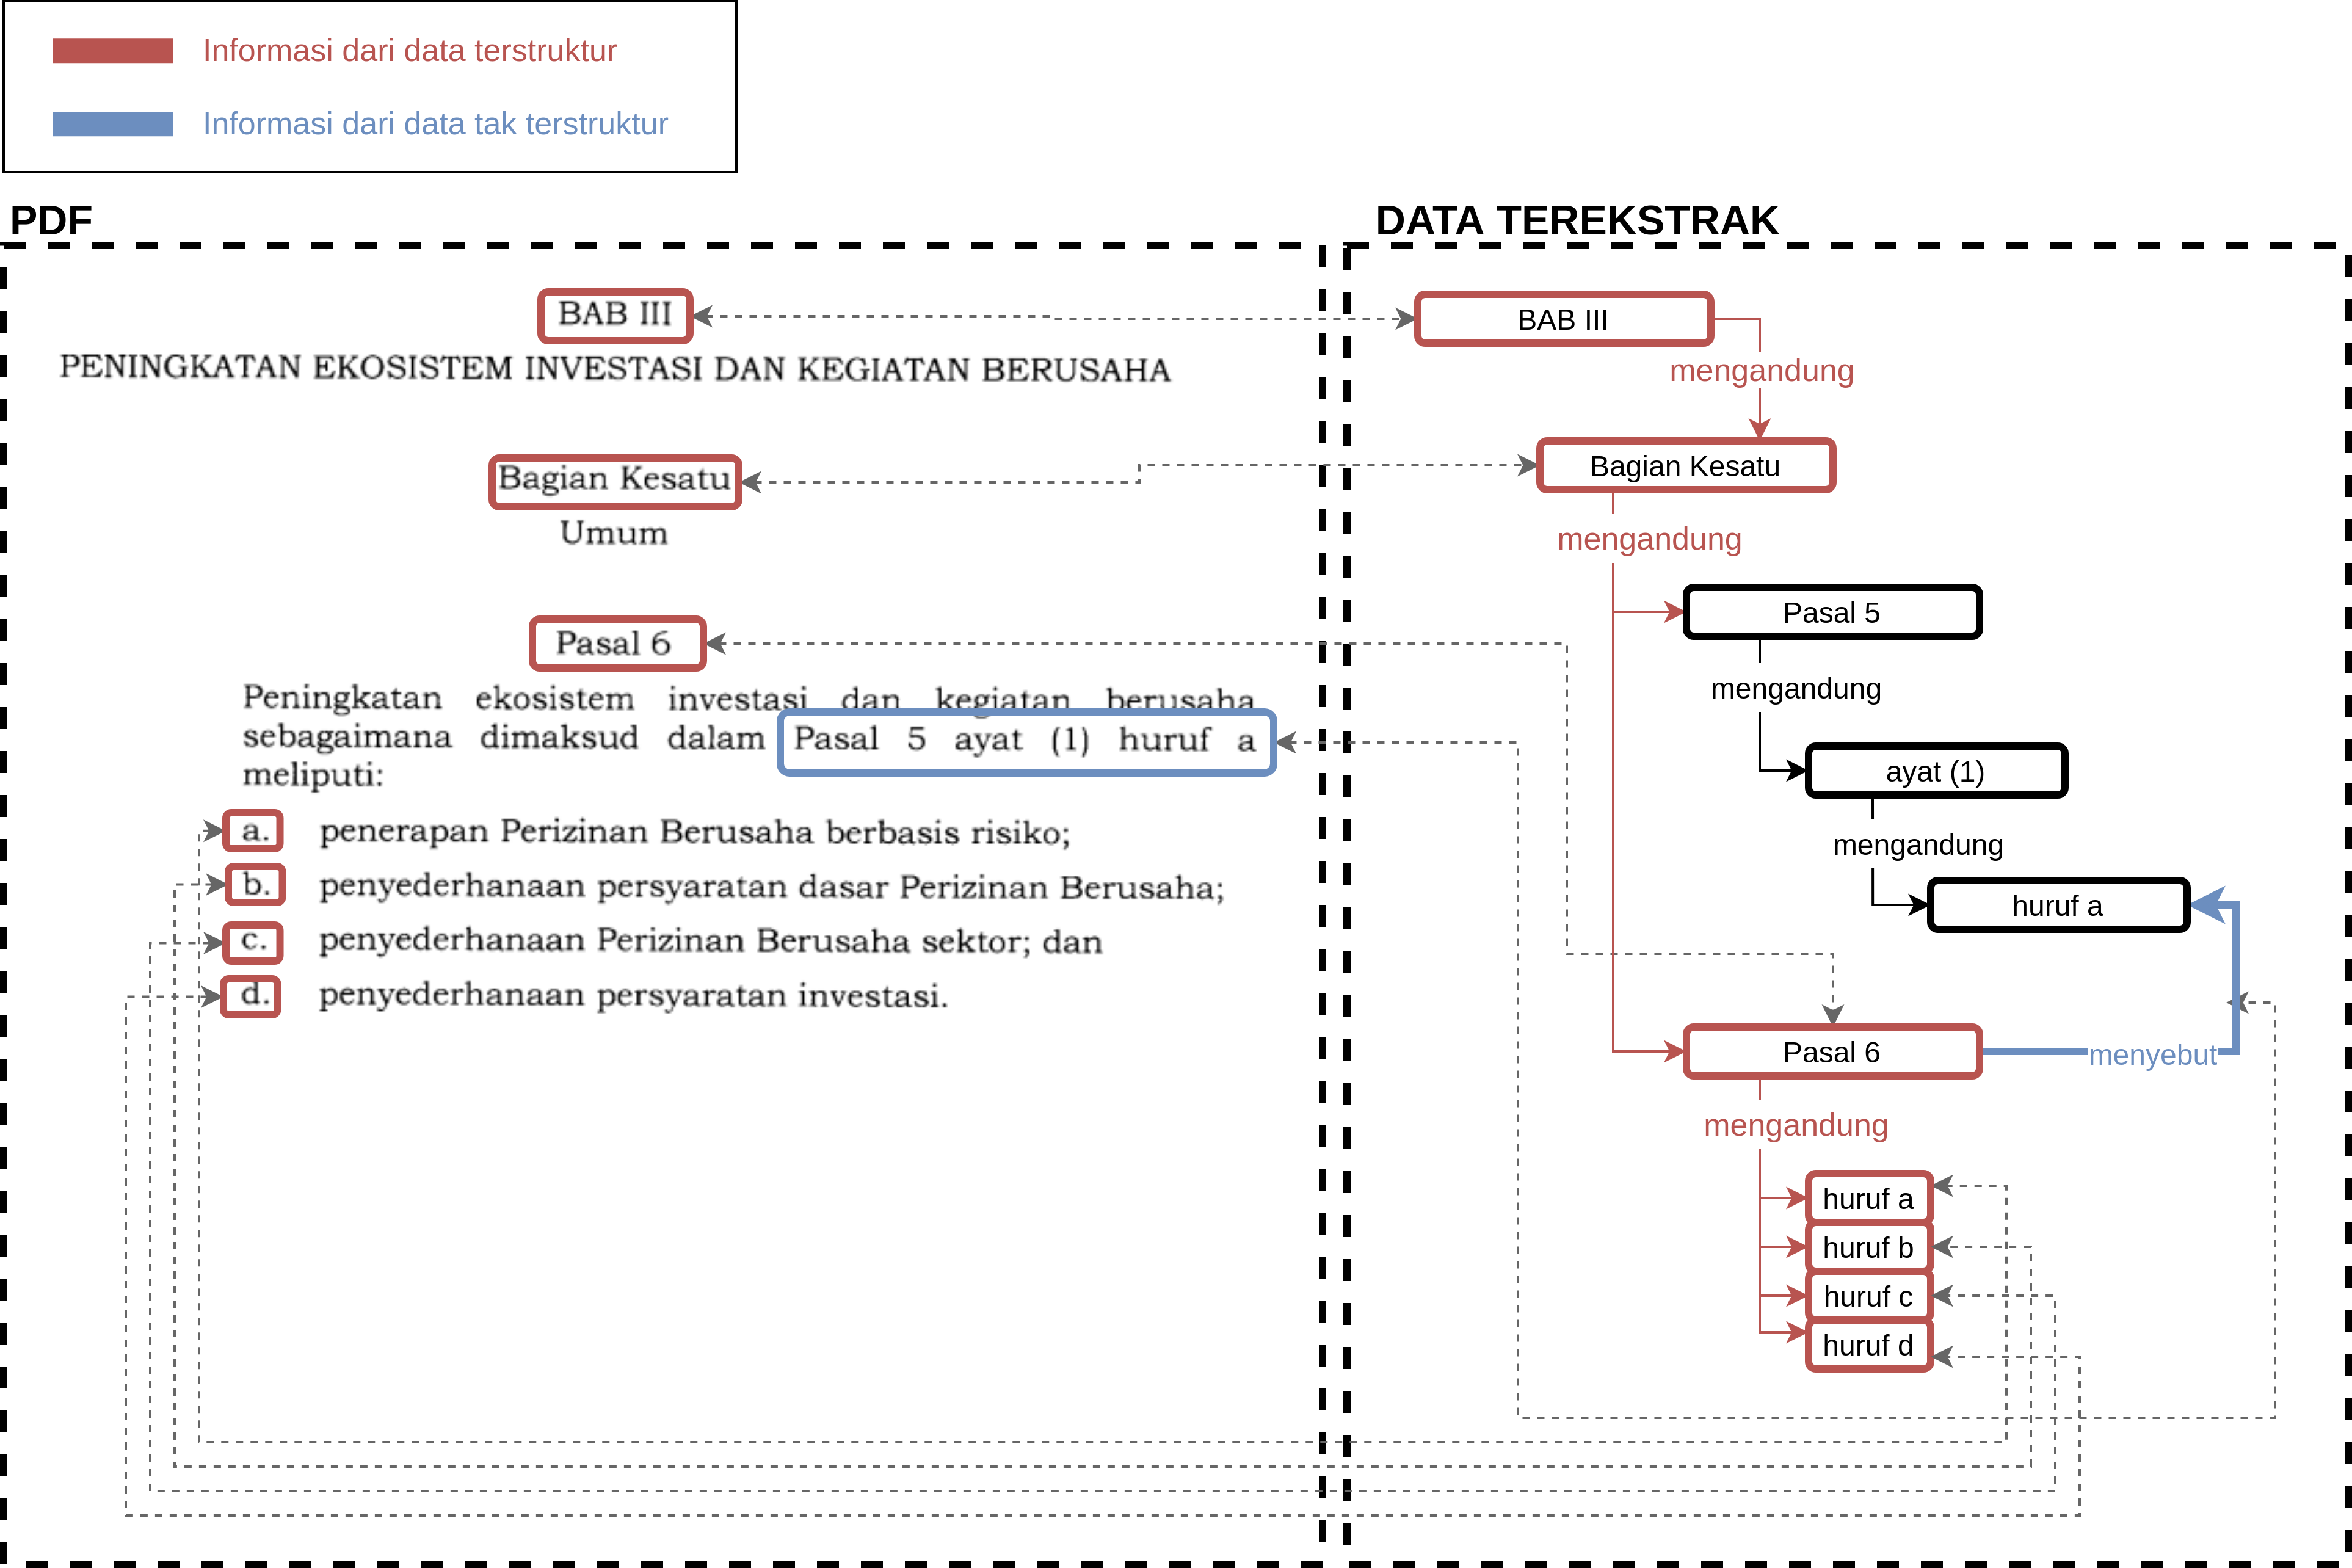
\includegraphics[width=\textwidth]{pictures/terstruktur.png}
  \caption{Cuplikan ekstraksi data terstruktur dan data tidak terstruktur dari dokumen PDF UU 11/2020 tentang Cipta Kerja}
  \label{fig:ekstraksi-dokumen}
\end{figure}

\pic~\ref{fig:ekstraksi-dokumen} menampilkan contoh ekstraksi informasi dari UU 11/2020 tentang
Cipta Kerja. Pada gambar tersebut terlihat bahwa terdapat dua jenis ekstraksi data yaitu ekstraksi
dari data terstruktur (merah) dan ekstraksi dari data tidak terstruktur (biru). Contoh data
terstruktur pada dokumen tersebut adalah \textit{section} pada dokumen seperti \textbf{Bab III},
\textbf{Bagian Kesatu}, \textbf{Pasal 6}, dan \textbf{huruf a - d}. Contoh data tidak terstruktur
pada dokumen tersebut adalah semua teks yang terdapat pada \textit{section} tersebut seperti teks
``penerapan Perizinan Berusaha berbasis risiko;'' yang terdapat pada \textbf{huruf a}. Manusia perlu
membaca manual untuk mengetahui bahwa UU 11/2020 mengandung \textbf{Bab III}, \textbf{Bab III}
mengandung \textbf{Bagian Kesatu}, \textbf{Bagian Kesatu} mengandung \textbf{Pasal 6}, dan
\textbf{Pasal 6} mengandung \textbf{huruf a - d}. Pada gambar tersebut, dalam mengekstraksi
informasi ``UU 11/2020 Pasal 6 merujuk kepada Pasal 5 ayat (1) huruf a'', manusia pertama-tama perlu
membaca dari awal teks pasal-pasal pada UU perujukan (citation), dan kemudian meng-\textit{infer}
informasi lengkap berdasarkan konteks \legal.

\begin{figure}[H]
  \centering
  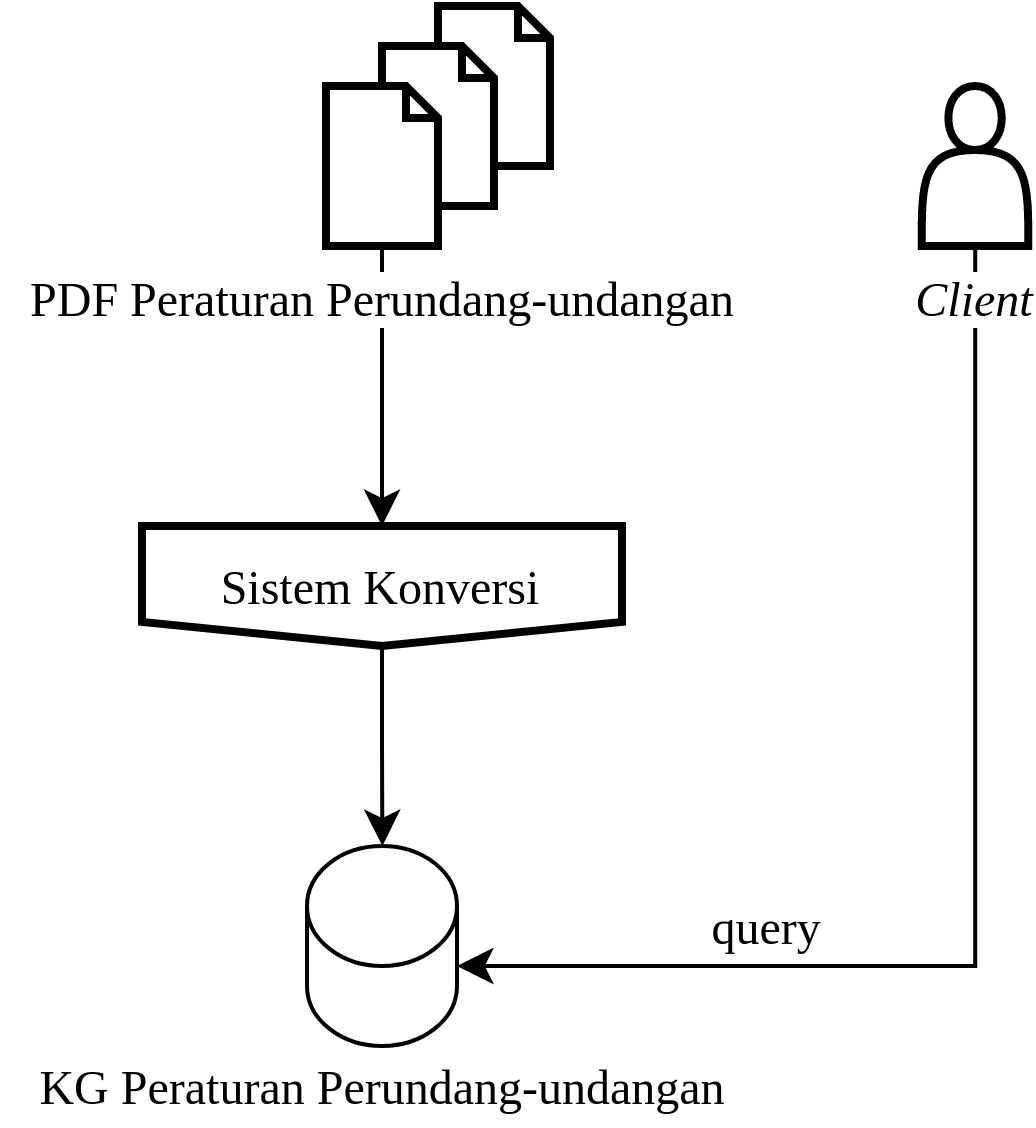
\includegraphics[scale=0.25]{pictures/konstruksi-dan-query.png}
  \caption{Bagan alir pembuatan dan \textit{query} KG \legal}
  \label{fig:konstruksi-dan-query}
\end{figure}

Data terstruktur yang digunakan dapat dalam berbagai format seperti JSON, XML, CSV, maupun skema
basis data SQL. Menurut \textit{5-star deployment scheme for Open
Data},\footnote{\url{https://5stardata.info/en/}} jenis data dapat dikategorikan menjadi 5 tingkat
yaitu \textit{1-star} hingga \textit{5-star}. \textit{5-star data} merupakan data dengan jenis
informasi paling bermanfaat, memberikan data dalam bentuk \textit{open license}, terstruktur,
tersedia dalam \textit{open format}, menggunakan URI sebagai notasi data, dan dapat dihubungkan
(\textit{linked}) dengan data lain. Pada penelitian ini penulis menggunakan \textit{Knowledge Graph}
sebagai struktur data hasil ekstraksi perundang-undangan, yang mana terkategori sebagai
\textit{5-star}. \textit{Knowledge graph} (KG) adalah struktur data yang (i) menggambarkan entitas
dunia nyata dan keterkaitannya, tersusun dalam bentuk \textit{graph}, (ii) mendefinisikan kelas
entitas dan relasi antar entitas dalam bentuk skema, (iii) membolehkan sembarang entitas memiliki
relasi satu sama lain dan (iv) mencakup berbagai topik domain \citep{paulheim_2016}. Dengan
melakukan ekstraksi data dari dokumen yang bersifat semi-terstruktur, \legal dapat dikonversi
menjadi KG. Sebagai manfaatnya, dapat fitur-fitur berbasis \textit{query} seperti \textit{question
answering}, \textit{reasoning} dan visualisasi data. \pic~\ref{fig:konstruksi-dan-query} menampilkan
garis besar dari peneilitan ini yaitu konstruksi KG \legal serta pemanfaatannya dari KG \legal
tersebut dalam yang dapat dilakukan dengan melakukan \textit{query}.

Untuk melakukan konversi dari PDF menjadi KG, secara umum dibutuhkan pemahaman struktur PDF tersebut
sehingga dapat dilakukan \textit{parsing} menjadi data yang dapat diproses oleh komputer, kemudian
dibutuhkan juga \textit{vocabulary} untuk menentukan KG seperti apa yang ingin dibuat. Spesifik pada
kasus \legal ini, penulis perlu mengetahui struktur serta konteks dari PDF peraturan
perundang-undangan, kemudian memerlukan \textit{vocabulary} spesifik untuk \legal yang menjadi dasar
pembuatan KG. Beberapa usaha telah dilakukan untuk membuat \textit{vocabulary} untuk KG \legal
seperti ELI,\footnote{\url{https://eur-lex.europa.eu/eli-register/about.html}}
Schema.org,\footnote{\url{https://schema.org}} dan
Wikidata.\footnote{\url{https://www.wikidata.org}}


\begin{listing}[H]
  \begin{minted}[fontsize=\scriptsize, frame=single, breaklines]{turtle}
@prefix schema: <http://schema.org/> .
@prefix xsd: <http://www.w3.org/2001/XMLSchema#> .

<http://data.europa.eu/eli/dir/1980/181/oj> a schema:Legislation ;
  schema:about <http://eurovoc.europa.eu/1896> ;
  schema:isBasedOn <http://njh.me/11957E100.html> ;
  schema:legislationDate "1979-12-20"^^schema:Date ;
  schema:legislationPassedBy "Council of the European Union"^^xsd:string ;
  schema:name "Council Directive 80/181/EEC of 20 December 1979 on the approximation of the laws of the Member States relating to units of measurement and on the repeal of Directive 71/354/EEC"^^xsd:string ;

<http://eurovoc.europa.eu/1896> a schema:Thing ;
  schema:name "Metrology"^^xsd:string .

<http://njh.me/11957E100.html> a schema:Legislation .
  \end{minted}
  \caption{Contoh KG metadata dokumen legal menggunakan \textit{vocabulary} Schema.org}
  \label{lst:schema-org-example}
\end{listing}

Pada \lst~\ref{lst:schema-org-example} diberikan contoh KG yang dibuat dengan \textit{vocabulary}
Schema.org. Contoh KG tersebut memuat metadata peraturan seperti tentang apa peraturan tersebut
(\code{schema:about}), apa dasar dari peraturan tersebut (\code{schema:isBasedOn}), dan nama dari
peraturan tersebut (\code{schema:name}). Akan tetapi, baik Schema.org maupun vocabulary-vocabulary
lainnya seperti pada ELI dan Wikidata, tidak dapat merepresentasikan struktur beserta isi peraturan.
Selain itu, \textit{vocabulary} tersebut dirancang secara generik, sehingga tidak dapat
merepresentasikan data yang secara spesifik terdapat pada \legal di Indonesia. Sehingga dengan
membuat \textit{vocabulary} untuk \legal di Indonesia, diharapkan dapat menjadi kontribusi dalam
memperluas penggunakan data struktur, terutama KG, dalam pembuatan dan pemeliharaan dokumen \legal.

Lex2KG merupakan \textit{framework} yang dikembangkan pada penelitian ini, dapat mengonversi dokumen
menjadi KG secara otomatis. Lex diambil dari Bahasa Latin yang artinya hukum, atau \textit{legal}
dalam Bahasa Inggris. Belum ada pekerjaan terkait yang melakukan automasi konversi dokumen \legal
menjadi KG secara otomatis. Oleh karena itu Lex2KG diharapkan dapat menjadi kontribusi yang
mendukung pembuatan dan penggunaan KG secara umum, dan bidang hukum secara khusus. Diluar dari
contoh \textit{use case} yang dijelaskan pada tulisan ini, KG yang dibuat oleh Lex2KG dapat
dikembangkan lebih lanjut dengan menggunakan kelebihan KG yaitu kemudahan untuk mengaitkan KG.
Sebagai contoh, data pada KG tentang peraturan dengan topik penyakit dapat dihubungkan dengan KG
penyakit untuk dapat dilakukan pencarian dalam pengetahuan yang lebih luas.

%--------------------------------------------------------------------------------------------------%
\section{Permasalahan}
\label{sec:permasalahan}
%--------------------------------------------------------------------------------------------------%

Berikut adalah rumusan permasalahan dari penelitian yang dilakukan:
\begin{itemize}
  \item Bagaimana membuat ontologi agar KG yang dihasilkan dapat menjawab \textit{competency questions}?
  \item Bagaimana merancang suatu sistem untuk melakukan konversi otomatis PDF \legal menjadi KG
        berdasarkan ontologi yang sudah dibuat?
  \item Bagaimana hasil konversi dan evaluasi terhadap KG \legal tersebut?
\end{itemize}

%--------------------------------------------------------------------------------------------------%
\section{Batasan Permasalahan}
\label{sec:batasan-permasalahan}
%--------------------------------------------------------------------------------------------------%

Berikut adalah batasan dari penelitian yang dilakukan:
\begin{itemize}
  \item Konversi hanya dapat dilakukan pada \legal di Indonesia
  \item Peraturan yang di-\textit{maintain} kualitas konversinya dibatasi kepada beberapa peraturan
        UU dan non-UU dengan format PDF yang sama dengan PDF yang diperoleh dari Laman Undang-Undang Jaringan
Dokumentasi dan Informasi Hukum DPR RI.
  \item Peraturan yang di-\textit{maintain} kualitas konversinya memiliki jumlah yang
        \textit{imbalanced} untuk UU dan peraturan jenis lainnya
  \item Tidak dapat melakukan \textit{query} terhadap KG yang kompleks seperti \textit{query} yang
        membutuhkan \textit{natural language processing} (contoh: ``Jika saya berusia 12 tahun,
        apakah saya boleh bekerja menurut UU Ketenagakerjaan?'') atau yang membutuhkan konteks
        semantik seperti \textit{abnormality/consistency detection}.
\end{itemize}

%--------------------------------------------------------------------------------------------------%
\section{Metodologi Penelitian}
\label{sec:metodologi-penelitian}
%--------------------------------------------------------------------------------------------------%

Metodologi penelitian dilakukan sesuai dengan yang diilustrasikan pada \pic~\ref{fig:metodologi}.
Perancangan sebuah KG dimulai dengan membuat \textit{competency questions}.


\begin{figure}
  \centering
  \begin{tikzpicture}[node distance=0.5cm]
    %Styles   
    \tikzstyle{r} = [rectangle, minimum width=7cm, minimum height=0.5cm, draw, text centered]

    %Nodes
    \node[r] (pertanyaan)                           {Merancang \textit{Competency Questions}};
    \node[r] (ontologi)     [below=of pertanyaan]   {Perancangan Ontologi};
    \node[r] (pengembangan) [below=of ontologi]     {Pengembangan Sistem Konversi};
    \node[r] (usecase)      [below=of pengembangan] {\textit{Use Case Evaluation}};

    %Lines
    \draw[->] (pertanyaan.south)   -- (ontologi.north);
    \draw[->] (ontologi.south)     -- (pengembangan.north);
    \draw[->] (pengembangan.south) -- (usecase.north);

  \end{tikzpicture}
  \caption{Metodologi Penelitian}
  \label{fig:metodologi}
\end{figure}

Setelah merancang \textit{competency questions}, penelitian dilenjutkan dengan merancang ontologi
(desain KG) yang dapat menjawab \textit{competency questions} tersebut. Ontologi ini kemudian akan
digunakan sebagai landasan sistem konstruksi KG. Karena sulit untuk menjamin hasil konversi untuk
semua PDF \legal, akan terdapat beberapa PDF yang akan di-\textit{maintain} kualitas konversinya
yang selanjutnya akan disebut \textit{maintained PDFs}. Pengembangan sistem konversi dilakukan
secara iteratif. Setiap terjadi perubahan pada sistem konversi, akan diperiksa apakah untuk semua
\textit{maintained PDFs} memberikan hasil konversi dengan kualitas yang tinggi. Sistem konversi akan
menerima input berupa PDF dan mengeluarkan output berupa KG dengan ontologi yang sudah dirancang
pada tahap sebelumnya.

Untuk menjamin KG yang dibuat dapat menjawab \textit{competency questions}, dalam penelitian ini
dilakukan \textit{use case evaluation} yaitu berupa demonstrasi contoh penerapan dari KG berdasarkan
\textit{competency questions}. Setelah semua \textit{competency questions} dapat terjawab oleh KG
dari \textit{maintained PDFs} dan dilakukan \textit{use case evaluation}, dilakukan \textit{large
scale evaluation} di mana PDF di luar \textit{maintained PDFs} akan dikonversi kemudian dilakukan
sampling pada hasil konversinya untuk dievaluasi secara kualitatif.

%--------------------------------------------------------------------------------------------------%
\section{Sistematika Penulisan}
\label{sec:sistematika-penulisan}
%--------------------------------------------------------------------------------------------------%

Penelitian ini dibagi ke dalam 6 bab bahasan. Bab pertama menjelaskan mengenai pendahuluan yang
berisikan latar belakang serta konteks penelitian yang dilakukan. Pada bab kedua dijelaskan mengenai
tinjauan pustaka yang dilakukan di mana dijelaskan berbagai istilah dan bidang ilmu yang berkaitan
dengan penelitian yang dilakukan. Lalu, pada bab ketiga dijelaskan mengenai perancangan penelitian
yang dilakukan dalam menyusun penelitian ini. Selanjutnya, bab keempat akan membahas implementasi
penelitian. Bab kelima akan membahas evaluasi dan analisis hasil penelitian. Bab keenam akan
membahas kesimpulan penelitian dan saran untuk penelitan selanjutnya.
\clearchapter
% -------------------------------------------------------------------------------------------------%
\chapter{TINJAUAN PUSTAKA}
\label{chap:2}
%--------------------------------------------------------------------------------------------------%

%--------------------------------------------------------------------------------------------------%
\section{Knowledge Graph}
\label{sec:knowledge-graph}
%--------------------------------------------------------------------------------------------------%

\textit{Knowledge graph} merupakan model data berbasis \textit{graph} yang menggambarkan entitas
dunia nyata dan hubungan antara entitas-entitas tersebut \citep{seth_2019}. Sebagai contoh, pada
\pic~\ref{fig:kg-description} dapat dilihat terdapat entitas-entitas yang ditandai dengan bentuk
lingkaran, dan hubungan antara entitas-entitas ditandai dengan bentuk anak panah. Pada gambar dapat
dilihat bahwa terdapat entitas "James" dan "Louvre" dan properti "has visited" yang mengarah dari
"James" ke "Louvre". Relasi tersebut dapat kita anggap sebagai sebuah pengetahuan yang dalam bahasa
manusia dapat dituliskan sebagai ``James pernah mengunjungi Louvre''. Model data seperti ini cocok
untuk menyimpan data dengan banyak jenis relasi antara entitas seperti pengetahuan umum,
dibandingkan dengan \textit{relational database} yang cocok untuk menyimpan data dengan relasi antar
entitas yang sudah diketahui dan terbatas.

\begin{figure}[H]
  \centering
  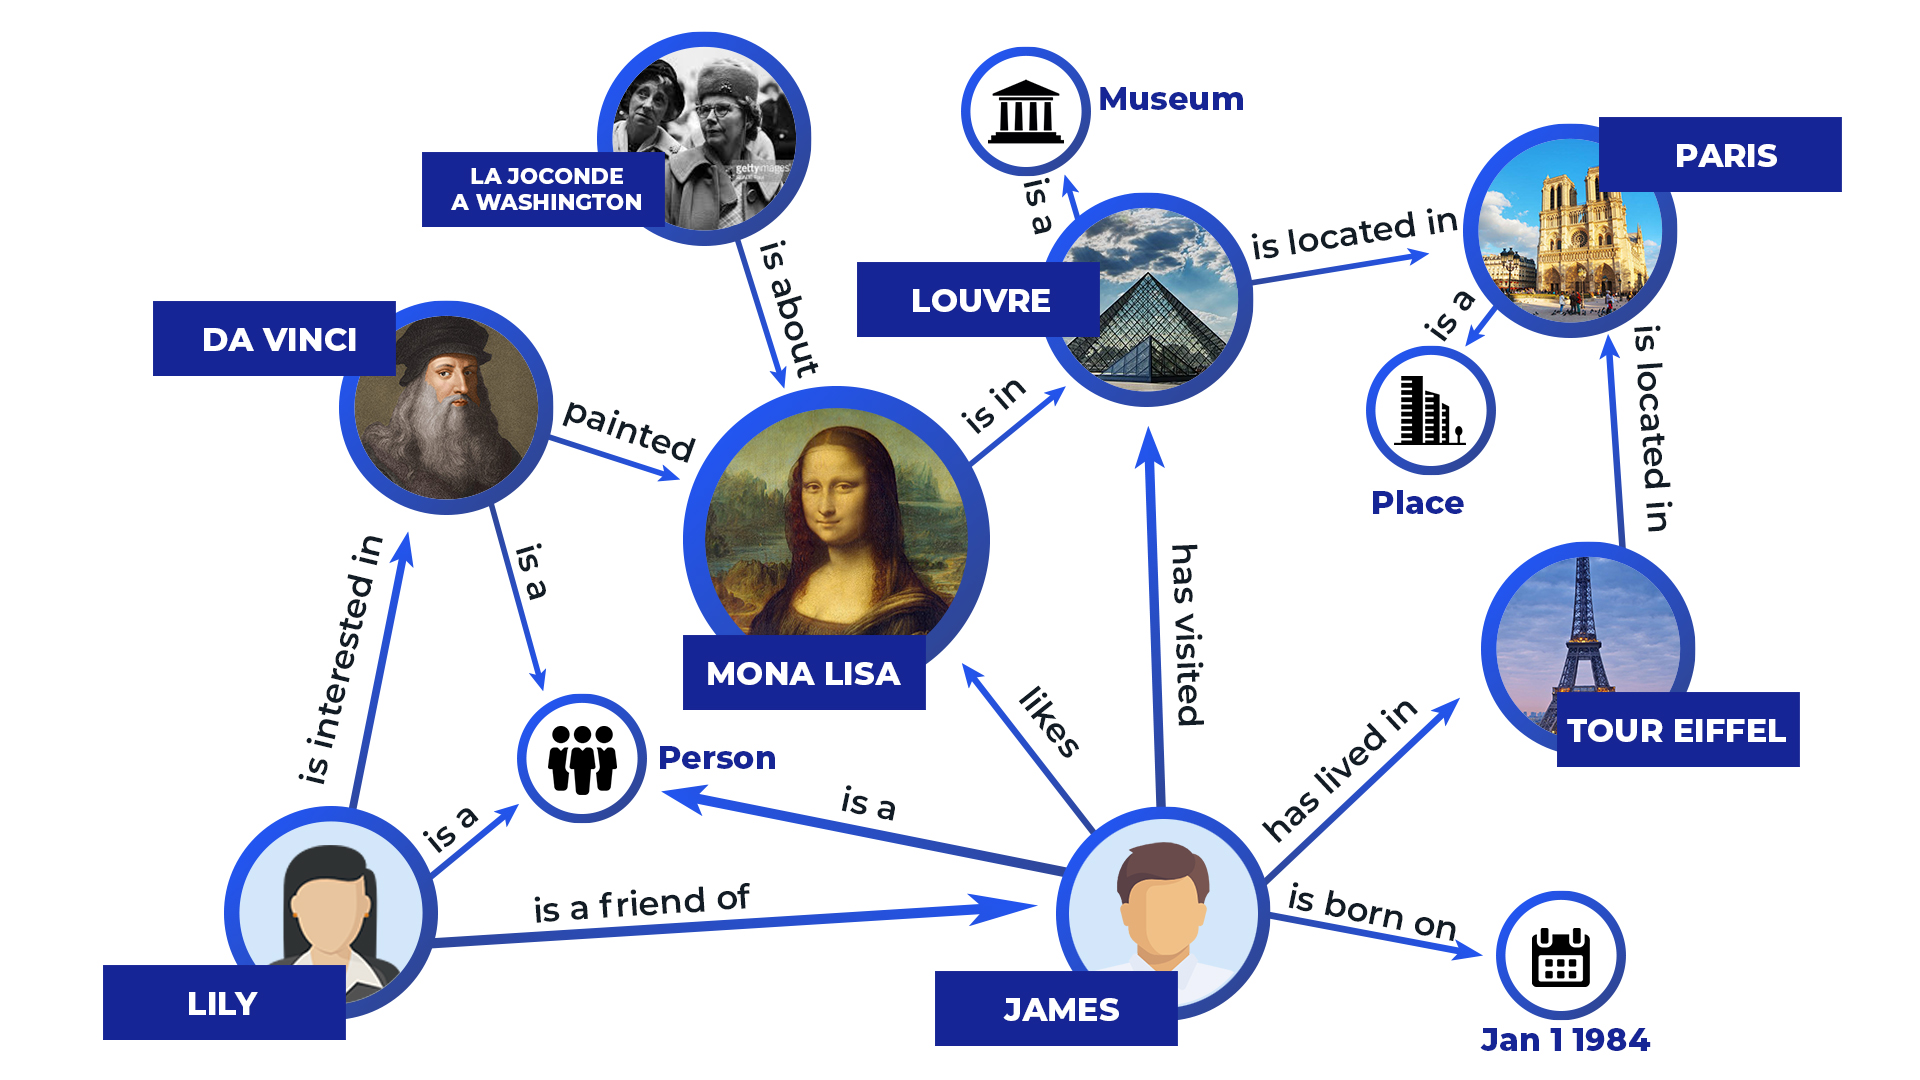
\includegraphics[width=\textwidth]{pictures/knowledge_graph.jpg}
  \caption[Contoh \textit{Knowledge Graph}]{Contoh \textit{Knowledge Graph}\\Sumber: \citep{seth_2019}}
  \label{fig:kg-description}
\end{figure}


%--------------------------------------------------------------------------------------------------%
\section{Resource Description Framework}
\label{sec:resource-description-framework}
%--------------------------------------------------------------------------------------------------%

Resource Description Framework (RDF) merupkan model data yang memberikan pernyataan tentang suatu
\textit{resource} dalam bentuk subjek-properti-objek, atau sering disebut \textit{triple}. Sebuah KG
dapat direpresentasikan sebagai kumpulan \textit{triple}. Subyek dan properti dalam \textit{triple}
direpresentasikan sebagai Uniform Resource Identifier (URI), sedangkan objek dapat direpresentasikan
dengan URI atau \textit{string literal}. Pada \pic~\ref{fig:triple-example}, dapat dilihat terdapat
KG dengan dua \textit{triple}. Pada \textit{Triple} 1, subjek, properti, dan objek berturut-turut
adalah \mono{https://example.org/James}, \mono{https://example.org/hasVisited},
\mono{https://example.org/Louvre} yang mana semuanya berbentuk URI. Sedangkan pada \textit{Triple}
2, subjek, properti, dan objek berturut-turut adalah \mono{https://example.org/James},
\mono{https://example.org/hasName}, "James". \mono{https://example.org/James},
\mono{https://example.org/Louvre} berturut-turut merupakan notasi untuk \textit{resource} entitas
James dan Louvre, \mono{https://example.org/hasVisited} dan \mono{https://example.org/hasName}
merupakan properti yang menjelaskan hubungan antara subjek dan objek, dan "James" adalah
\textit{string literal} yang menunjukan nilai dari nama James.

\begin{figure}
  \centering
  \begin{tikzpicture}[node distance=2cm and 1cm]
    %Styles   
    \tikzstyle{r} = [rectangle, minimum width=6cm, minimum height=0.5cm, draw, text centered]

    %Nodes
    \node[r] (james1)                      {\texttt{https://example.org/James}};
    \node[r] (louvre)    [below=of james1] {\texttt{https://example.org/Louvre}};
    \node[r] (james2)    [right=of james1] {\texttt{https://example.org/James}};
    \node[r] (james-str) [below=of james2] {"James"};

    %Lines
    \draw[->] (james1.south)   -- node {\colorbox{white}{\texttt{https://example.org/hasVisited}}} (louvre.north);
    \draw[->] (james2.south)   -- node {\colorbox{white}{\texttt{https://example.org/hasName}}} (james-str.north);

    %Boxes
    \node[draw, dashed, inner sep=10pt, label={Triple 1}, fit=(james1) (louvre)] {};
    \node[draw, dashed, inner sep=10pt, label={Triple 2}, fit=(james2) (james-str)] {};
  \end{tikzpicture}
  \caption{Contoh \textit{triple}}
  \label{fig:triple-example}
\end{figure}



Terdapat beberapa format berkas dan sintaks untuk mengekspresikan RDF. Pada penelitian ini, penulis
menggunakan format Terse RDF Triple Language (Turtle) \citep{turtle}. Sebagai contoh, KG pada
\pic~\ref{fig:triple-example} dapat dituliskan dalam format Turtle seperti
\lst~\ref{lst:contoh-ttl}.

\begin{listing}[H]
  \begin{minted}[fontsize=\scriptsize, frame=single, breaklines]{turtle}
<https://example.org/James> <https://example.org/hasVisited> <https://example.org/Louvre> .
<https://example.org/James> <https://example.org/hasName> "James" .
\end{minted}
  \caption{Contoh penulisan \textit{triple} dalam Turtle}
  \label{lst:contoh-ttl}
\end{listing}

Dengan fitur format Turtle, dua \textit{triple} pada \lst~\ref{lst:contoh-ttl} dapat ditulis lebih
singkat dengan mengganti prefix URI yang sama menjadi teks yang lebih singkat, dan menggabungkan
penulisan beberapa \textit{triple} dengan subjek yang sama sehingga subjek hanya perlu dituliskan
sekali saja. Sebagai contoh, karena sebagaian besar URI memiliki prefix \mono{https://example.org/},
kita dapat menggantinya dengan \textit{string} \mono{ex:} dengan mendeklarasikan
\mono{@prefix ex: https://example.org/ .}. Selanjutnya \mono{ex:} digunakan sebagai notasi singkat
\mono{https://example.org/} untuk mempermudah pembacaan. Kedua \textit{triple} juga memiliki subjek
yang sama yaitu \mono{ex:James}, oleh karena itu, penulisan kedua Turtle bisa digabung dengan hanya
menuliskan subjek sebanyak satu kali, kemudian menuliskan properti dan objek dipisah dengan tanda
titik koma. \lst~\ref{lst:contoh-singkat-ttl} adalah contoh penulisan \lst~\ref{lst:contoh-ttl}
dalam bentuk yang lebih singkat dan lebih mudah dibaca oleh manusia.

\begin{listing}[H]
  \begin{minted}[fontsize=\scriptsize, frame=single]{turtle}
@prefix ex: <https://example.org/> .

ex:James 
  ex:hasVisited ex:Louvre ;
  ex:hasName "James" .
\end{minted}
  \caption{Contoh penulisan lebih singkat sebuah \textit{triple} dalam Turtle}
  \label{lst:contoh-singkat-ttl}
\end{listing}


%--------------------------------------------------------------------------------------------------%
\section{SPARQL}
\label{sec:sparql}
%--------------------------------------------------------------------------------------------------%

SPARQL merupakan salah satu RDF \textit{query language} yaitu bahasa yang mampu mengambil atau
mengubah data yang disimpan dalam format RDF. Sintaks SPARQL memiliki beberapa kesamaan dengan SQL,
contohnya sebuah variabel diawali dengan tanda tanya seperti \mono{?name}. Query SPARQL sederhana
dapat dibentuk dengan \mono{SELECT} dan \mono{WHERE} dengan kondisi pola triple ditulis di dalam
\mono{WHERE} dan variabel yang akan ditampilkan ditulis didalam \mono{SELECT}\citep{owlizr}. Berikut
adalah penjelasan singkat \textit{clause} SPARQL yang digunakan pada penelitian ini.

\begin{itemize}
  \itemsep1pt\parskip0pt\parsep0pt
  \item \mono{PREFIX}: Mendeklarasikan pemetaan prefix URI menjadi \textit{string} yang lebih
        singkat. Hal ini dilakukan agar \textit{query} lebih mudah dibaca oleh manusia seperti sintaks
        \mono{@prefix} pada Turtle.
  \item \mono{SELECT}: Menyatakan variabel yang akan ditampilkan sebagai output dari \textit{query}.
  \item \mono{WHERE}: Menyatakan kondisi \textit{triple} yang akan ditampilkan pada output. Elemen
        dari \textit{triple} yaitu subjek, predikat, dan objek dapat beruba vaiable atau
        \textit{fixed value} seperti \textit{string} atau bilangan.
  \item \mono{FILTER}: Mengeliminasi solusi yang tidak membuat \textit{expression} bernilai
        \textit{true}.
  \item \mono{UNION}: \mono{{A} UNION {B}} menggabungkan \textit{triple} dari A dan B.
  \item \mono{MINUS}: \mono{A MINUS {B}} hanya memuat \textit{triple} pada A yang tidak
        \textit{non compatible} dengan B.
\end{itemize}

SPARQL juga memiliki fitur \textit{property path} yang mempermudah penulisan query. Jenis-jenis
\textit{property path} dapat dilihat pada \pic~\ref{fig:pp}.

\begin{figure}[H]
  \centering
  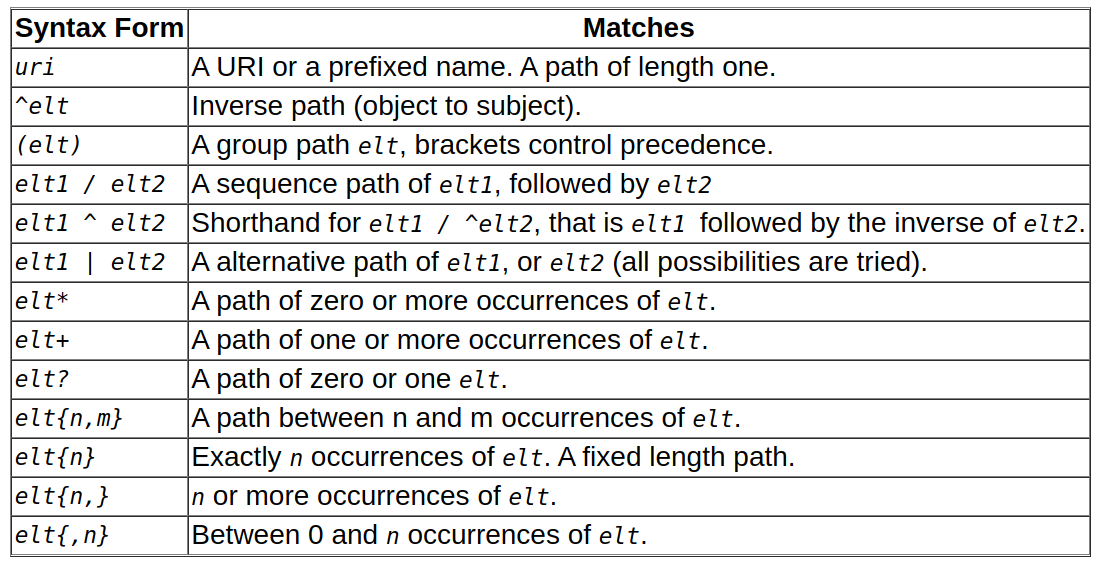
\includegraphics[width=0.8\textwidth]{pictures/pp.png}
  \caption[Property path SPARQL]{Property path SPARQL\\Sumber: \citep{sparql}}
  \label{fig:pp}
\end{figure}

Berikut adalah contoh-contoh \textit{query} SPARQL yang dilakukan pada contoh KG pada
\lst~\ref{lst:contoh-singkat-ttl}.

%--------------------------------------------------------------------------------------------------%
\subsection{Contoh Query 1}
\label{sec:contoh-query-1}
%--------------------------------------------------------------------------------------------------%

\lst~\ref{lst:query-1} merupakan SPARQL \textit{query} untuk menampilkan semua \textit{triple} yang terdapat
pada KG, akan memberikan output \tab~\ref{tab:output-query-1}. Setiap baris yang terdapat pada
output merupakan \textit{triple} yang tedapat pada KG.

\begin{listing}[H]
  \begin{minted}[fontsize=\scriptsize, frame=single]{sparql}
PREFIX ex: <https://example.org/>
SELECT ?subjek ?predikat ?objek
WHERE { ?subjek ?predikat ?objek }
  \end{minted}
  \caption{Query 1}
  \label{lst:query-1}
\end{listing}


\begin{table}
  \centering
  \begin{tabular}{|l|l|l|} \hline
    ?subjek           & ?predikat              & ?objek             \\\hline \hline
    \texttt{ex:James} & \texttt{ex:hasVisited} & \texttt{ex:Louvre} \\\hline
    \texttt{ex:James} & \texttt{ex:hasName}    & "James"            \\\hline
  \end{tabular}
  \caption{Output Query 1}
  \label{tab:output-query-1}
\end{table}

%--------------------------------------------------------------------------------------------------%
\subsection{Contoh Query 2}
\label{sec:contoh-query-2}
%--------------------------------------------------------------------------------------------------%

\lst~\ref{lst:query-2} merupakan SPARQL \textit{query} untuk menampilkan semua properti dan objek
pada \textit{triple} dengan subjek \mono{ex:James}. pada KG, akan memberikan output
\tab~\ref{tab:output-query-2}.

\begin{listing}[H]
  \begin{minted}[fontsize=\scriptsize, frame=single]{sparql}
PREFIX ex: <https://example.org/>
SELECT ?properti ?objek
WHERE { ex:James ?properti ?objek }
  \end{minted}
  \caption{Query 2}
  \label{lst:query-2}
\end{listing}

\begin{table}
  \centering
  \begin{tabular}{|l|l|} \hline
    ?properti              & ?objek             \\\hline \hline
    \texttt{ex:hasVisited} & \texttt{ex:Louvre} \\\hline
    \texttt{ex:hasName}    & "James"            \\\hline
  \end{tabular}
  \caption{Output Query 3}
  \label{tab:output-query-2}
\end{table}

%--------------------------------------------------------------------------------------------------%
\subsection{Contoh Query 3}
\label{sec:contoh-query-3}
%--------------------------------------------------------------------------------------------------%

\lst~\ref{lst:query-3} merupakan SPARQL \textit{query} untuk menampilkan semua objek pada
\textit{triple} dengan subjek \mono{ex:James} dan properti \mono{ex:hasVisited}, dengan output
\tab~\ref{tab:output-query-3}. Artinya, \textit{query} ini menampilkan semua tempat yang pernah
dikunjungi James, yaitu Louvre.

\begin{listing}[H]
  \begin{minted}[fontsize=\scriptsize, frame=single]{sparql}
PREFIX ex: <https://example.org/>
SELECT ?visited_place
WHERE { ex:James ex:hasVisited ?visited_place }
  \end{minted}
  \caption{Query 3}
  \label{lst:query-3}
\end{listing}

\begin{table}
  \centering
  \begin{tabular}{|l|l|l|} \hline
    \texttt{?visited\_place} \\ \hline \hline
    \texttt{ex:Louvre}       \\ \hline
  \end{tabular}
  \caption{Output Query 3}
  \label{tab:output-query-3}
\end{table}

%--------------------------------------------------------------------------------------------------%
\subsection{Contoh Query 4}
\label{sec:contoh-query-4}
%--------------------------------------------------------------------------------------------------%

\textit{Query} ini merupakan \textit{query} yang relatif kompleks yang akan dilakukan terhadap
\textit{server} SPARQL wikidata. Pada \textit{query} ini dilakukan pencarian artikel wikipedia dalam
dua bahasa yaitu ``en'' dan ``uz'', di mana artikelnya adalah tentang \mono{wd:Q5} yaitu manusia.

\begin{listing}[H]
  \begin{minted}[fontsize=\scriptsize, frame=single]{sparql}
SELECT DISTINCT ?lang ?name WHERE {
  ?article schema:about wd:Q5 ;
              schema:inLanguage ?lang ;
              schema:name ?name ;
              schema:isPartOf [ wikibase:wikiGroup "wikipedia" ] .
  FILTER(?lang in ('en', 'uz')) .
  \end{minted}
  \caption{Query 4}
  \label{lst:query-4}
\end{listing}

\begin{table}
  \centering
  \begin{tabular}{|l|l|} \hline
    lang & name \\ \hline \hline
    uz & Odam \\ \hline
    en & Human \\ \hline
  \end{tabular}
  \caption{Output Query 4}
  \label{tab:output-query-4}
\end{table}

%--------------------------------------------------------------------------------------------------%
\section{\Legal}
\label{sec:legal}
%--------------------------------------------------------------------------------------------------%

Menurut Pasal 7 Ayat 1 UU 10/2004 tentang pembentukan \legal, \legal adalah peraturan tertulis yang
dibentuk oleh lembaga negara atau pejabat yang berwenang dan mengikat secara umum. Jenis dan
hierarki \legal terdiri atas:

\begin{enumerate}
  \item Undang-Undang Dasar Negara Republik Indonesia Tahun 1945
  \item Undang-Undang/Peraturan Pemerintah Pengganti Undang-Undang
  \item Peraturan Pemerintah
  \item Peraturan Presiden
  \item Peraturan Daerah
\end{enumerate}

Berikut adalah beberapa peranan perundang-undangan untuk Indonesia \citep{ilmu_perundang_undangan}:

\begin{itemize}
  \item \Legal merupakan kaidah hukum yang mudah dikenal (diidentifikasi),
        mudah diketemukan kembali, dan mudah ditelusuri. Sebagai kaidah hukum tertulis, bentuk,
        jenis,dan tempatnya jelas. Begitu pula pembuatnya.
  \item \Legal memberikan kepastian hukum yang lebih nyata karena
        kaidah-kaidahnya mudah diidentifikasi dan mudah diketemukan kembali.
  \item Struktur dan sistematika \legal lebih jelas sehingga memungkinkan
        untuk diperiksa kembali dan diuji baik segi-segi formal maupun materi muatannya.
  \item Pembentukan dan pengembangan \legal dapat direncanakan. Faktor ini
        sangat penting bagi negara-negara yang sedang membangun termasuk membangun sistem hukum baru yang
        sesuai dengan kebutuhan dan perkembangan masyarakat.
\end{itemize}

Menurut lampiran UU 10/2004, struktur \legal terdiri atas:

\begin{itemize}
  \item Judul
  \item Pembukaan
  \item Batang Tubuh
  \item Penutup
  \item Penjelasan (jika diperlukan)
  \item Lampiran (jika diperlukan)
\end{itemize}

Bagian judul, pembukaan, dan penutup memuat metadata dari \legal tersebut seperti jenis, nomor,
tahun pengundangan atau penetapan, nama, jabatan pembentuk, konsiderans, kasar Hukum, \legal.
Konsiderans memuat uraian singkat mengenai pokok-pokok pikiran yang menjadi latar belakang dan
alasan pembuatan \legal. Dasar Hukum memuat dasar kewenangan pembuatan \legal dan \legal yang
memerintahkan pembuatan \legal tersebut. Oleh karena itu, kita dapat melihat keterkaitan antara
\legal dengan melihat konsiderans dan dasar hukum dari peraturan tersebut.

Batang tubuh \legal memuat semua substansi \legal yang dirumuskan dalam pasal. Pengelompokkan materi
\legal dapat disusun secara sistematis dalam buku, bab, bagian, dan paragraf atas dasar kesamaan
materi. Pasal dapat dirinci ke dalam beberapa ayat. Pasal dan ayat dapat dibuat dalam bentuk kalimat
maupun tabulasi rincian. Dalam bentuk tabulasi rincian, setiap rincian harus dapat dibaca sebagai
satu rangkaian kesatuan dengan frase pembuka dan setiap rincian diawali dengan huruf (abjad) kecil
dan diberi tanda baca titik. Suatu rincian dapat dibagi lagi ke unsur rincian yang lebih kecil.

Amendemen (perubahan) dapat dilakukan pada suatu \legal. Secara teoritis, perubahan konstitusi
(\textit{constitutional amendment}) mengandung tiga macam arti: 1) Menjadikan lain bunyi kalimatnya;
2) Menambahkan sesuatu yang baru, dan; 3) Ketentuan daman Undang-Undang Dasar dilaksanakan tidak
seperti yang tercantum di dalamnya\citep{teori_amandemen}. Bentuk amendemen dapat berupa pengubahan,
penyisipan, dan penghapusan. Amendemen juga dapat dilakukan pada tingkat peraturan maupun komponen
peraturan seperti pasal dan bab.

%--------------------------------------------------------------------------------------------------%
\section{\textit{European Legislation Identifier} (ELI)}
\label{sec:eli}
%--------------------------------------------------------------------------------------------------%

Negara-negara anggota EU memiliki cara mengatur informasi hukum yang berbeda-beda, sehingga
cenderung menghalangi penemuan, pertukaran, dan penggunaan kembali informasi. European Legislation
Identifier (ELI) adalah solusi yang bertujuan untuk mengatasi masalah-masalah tersebut. ELI
merupakan sistem untuk membuat \legal tersedia secara daring dalam format terstandardisasi, sehingga
dapat diakses dan digunakan oleh berbagai instansi \citep{eli}. ELI bertujuan untuk untuk
memfasilitasi akses, berbagi dan interkoneksi informasi hukum yang diterbitkan melalui nasional,
Eropa dan sistem informasi hukum global. ELI dibangun berdasarkan persetujuan antara negara-negara
EU.

ELI juga memiliki \textit{technical implementation
  guide}\footnote{\url{https://publications.europa.eu/en/publication-detail/-/publication/8159b75d-5efc-11e8-ab9c-01aa75ed71a1}}
yang menjelaskan implementasi ELI dan spesifikasi yang tedapat pada ELI. Spesifikasi ELI antara lain
adalah cara membuat URI suatu \textit{resource}, \textit{class}, dan properti. Ontologi yang
digunakan pada ELI cenderung untuk menjelaskan metadata dari peraturan, dan tidak memiliki pemodelan
khusus untuk menjelaskan \textit{subdivision} dari peraturan. Nyatanya, ELI menggunakan class
\textit{eli:LegalResourceSubdivision} untuk mendefinisikan semua \textit{subdivision}, tidak
terdapat kelas khusus untuk variasi \textit{subdivision} seperti bab, pasal, dan ayat. Selain itu,
ELI dirancang untuk digunakan pada peraturan di Eropa, sehingga tidak memiliki ontologi untuk jenis
peraturan di Indonesia seperti ``Peraturan Pemerintah''.

%--------------------------------------------------------------------------------------------------%
\section{Schema.org}
\label{sec:schema-org}
%--------------------------------------------------------------------------------------------------%

Schema.org adalah aktivitas komunitas kolaboratif dengan misi untuk membuat, memelihara, dan
mempromosikan skema untuk data terstruktur di internet, di halaman web, dalam pesan email, dan lebih
dari itu \citep{schema.org}. \textit{Vocabulary} Schema.org dapat digunakan dengan \textit{encoding}
yang berbeda, termasuk RDFa, Microdata dan JSON-LD. Banyak aplikasi dari Google, Microsoft,
Pinterest, Yandex, dan lainnya sudah menggunakan \textit{vocabulary} ini untuk memperkuat pengalaman
yang kaya dan dapat diperluas. Schema.org memiliki \textit{vocabulary} tersendiri untuk
\legal.\footnote{\url{https://schema.org/Legislation}} Salah satu \textit{vocabulary} nya adalah
properti yang menjelaskan metadata suatu \legal seperti \mono{legislationDate} dan
\mono{jurisdiction}.

%--------------------------------------------------------------------------------------------------%
\section{Wikidata}
\label{sec:wikidata}
%--------------------------------------------------------------------------------------------------%

Wikidata adalah basis pengetahuan \textit{free} dan terbuka yang dapat dibaca dan diedit oleh
manusia dan mesin \citep{wikidata}. Wikidata berperan sebagai penyimpanan pusat untuk data
terstruktur dari proyek saudara Wikimedia termasuk Wikipedia, Wikivoyage, Wiktionary, Wikisource,
dan lainnya. WikiProject adalah organisasi yang didirikan untuk mencapai tujuan penyuntingan
tertentu, atau untuk mencapai tujuan yang berkaitan dengan bidang pengetahuan tertentu. Terdapat
WikiProject tersendiri untuk bidang hukum dan \legal yaitu WikiProject
Law.\footnote{\url{https://www.wikidata.org/wiki/Wikidata:WikiProject_Law}} WikiProject Law
menyediakan properti terkait \legal sebagaimana yang dapat dilihat pada \pic~\ref{fig:wikiproject}
dan beberapa deskripsinya pada \tab~\ref{tab:wp-desc}.

\begin{figure}[H]
  \centering
  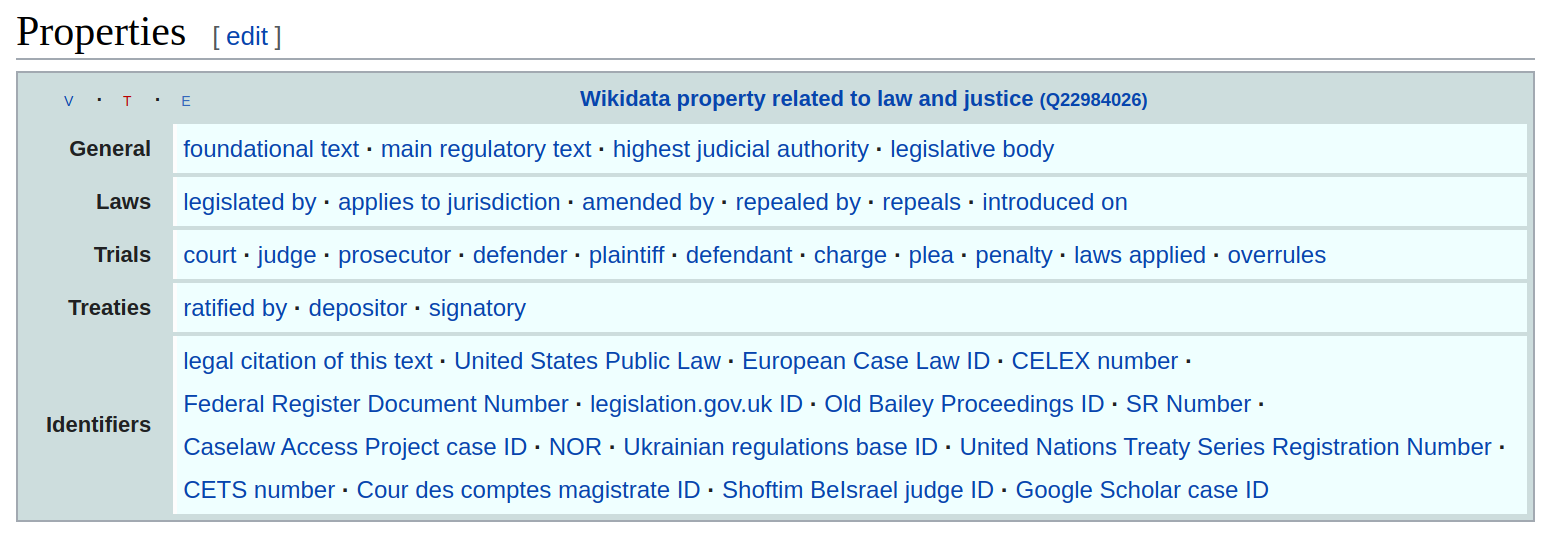
\includegraphics[width=0.8\textwidth]{pictures/wikiproject.png}
  \caption{Properti WikiProject Law}
  \label{fig:wikiproject}
\end{figure}

\begin{table}
  \centering
  \begin{tabular}{|p{0.2\textwidth}|p{0.8\textwidth}|} \hline
    label                   & deskripsi                                                                                                                                                                                          \\\hline \hline
    amended by              & document is amended by specified other document                                                                                                                                                    \\\hline
    legislated by           & indicates that an act or bill was passed by a legislature. The value can be a particular session of the legislature                                                                                \\\hline
    applies to jurisdiction & the item (institution, law, public office, public register...) or statement belongs to or has power over or applies to the value (a territorial jurisdiction: a country, state, municipality, ...) \\\hline
  \end{tabular}
  \caption{Deskripsi beberapa Properti WikiProject Law}
  \label{tab:wp-desc}
\end{table}


\clearchapter
%--------------------------------------------------------------------------------------------------%
\chapter{PERANCANGAN}
\label{chap:3}
%--------------------------------------------------------------------------------------------------%

Bab ini berisi perancangan arsitektur konversi, ontologi KG yang dihasilkan, dikaitkan dengan
\textit{competency questions}. \textit{Competency questions} harus diperjelas untuk dijadikan
landasan ontologi KG. KG yang dihasilkan oleh sistem konversi, digabung dengan ontologi yang sudah
dirancang harus dapat menjawab semua pertanyaan pada \textit{competency questions}.

%--------------------------------------------------------------------------------------------------%
\section{Arsitektur Sistem Konversi}
\label{sec:arsitektur-sistem-konversi}
%--------------------------------------------------------------------------------------------------%

\begin{figure}
  \centering
  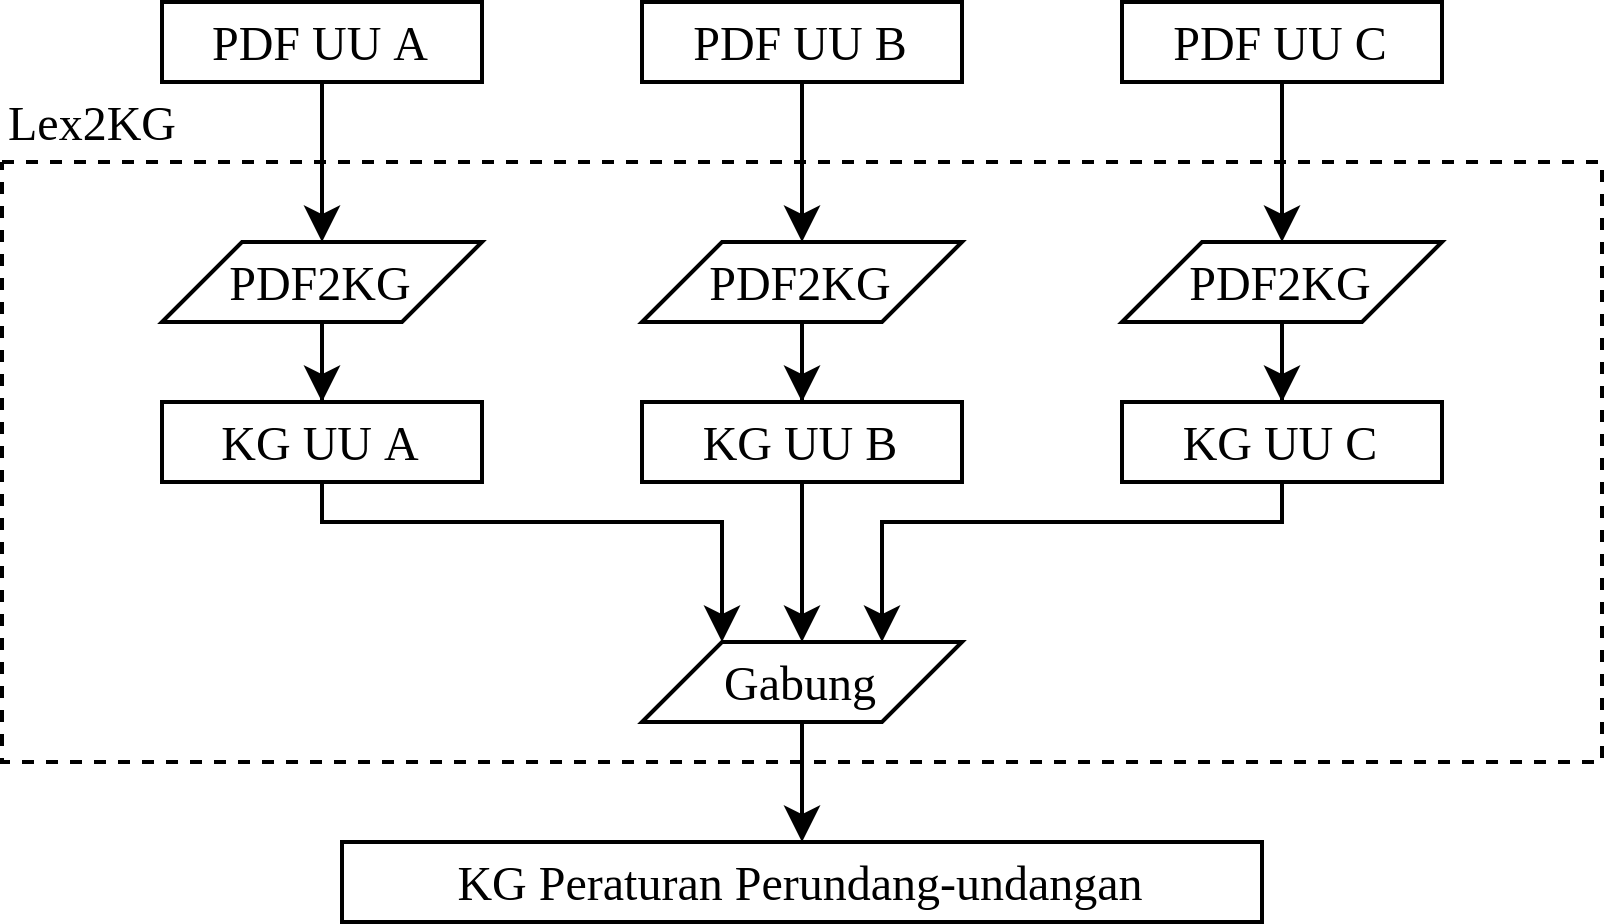
\includegraphics[scale=0.35]{pictures/lex2kg.png}
  \caption{Arsitektur Lex2KG}
  \label{fig:lex2kg}
\end{figure}

Lex2KG melakukan konversi masing-masing PDF \legal menjadi KG menggunakan modul PDF2KG kemudian KG
dari masing-masing PDF digabung dan dikeluarkan sebagai satu KG, seperti yang terlihat pada
\pic~\ref{fig:lex2kg}. KG dikeluarkan dalam format RDF Turtle di mana setiap barisnya merupakan
\textit{triple} yang terdapat pada KG, sehingga penggabungan KG dapat dilakukan dengan mudah yaitu
dengan menggabungkan baris-baris tersebut ke dalam satu berkas. 

\begin{figure}
  \centering
  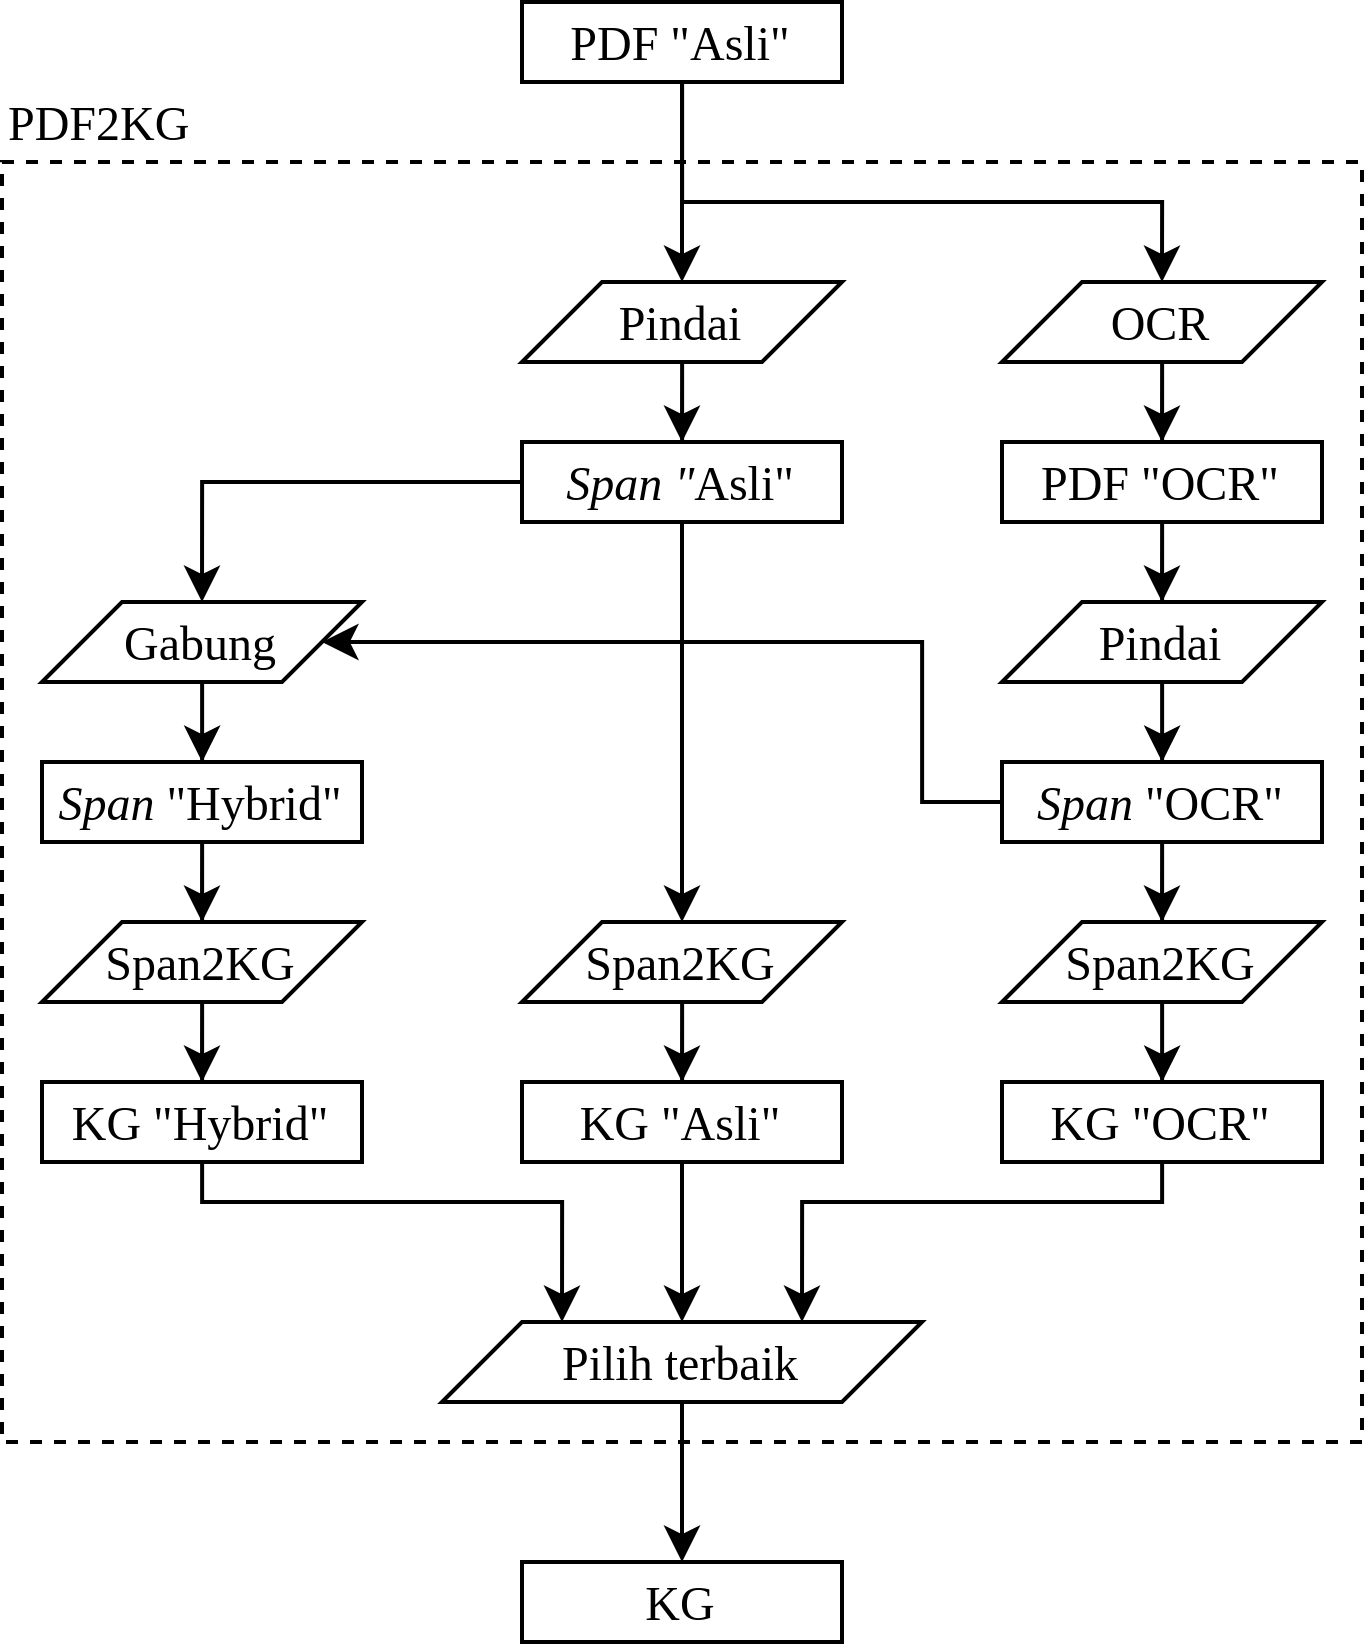
\includegraphics[scale=0.35]{pictures/pdf2kg.png}
  \caption{Arsitektur PDF2KG}
  \label{fig:pdf2kg}
\end{figure}

PDF2KG memiliki arsitektur seperti yang ditunjukan pada \pic~\ref{fig:pdf2kg}. Bagian
\textit{Optical Character Recognition} (OCR) bertanggung jawab untuk mengubah \textit{image-only}
PDF ("Asli) menjadi \textit{text-scannable} PDF ("OCR") dan menstandardisasi pemformatan semua PDF.
Selanjutnya kedua file PDF "Asli" dan "OCR" dipindai untuk mengekstrak teks beserta posisinya, yang
selanjutnya disebut \textit{span}. Kemudian \textit{span} "Asli" dan \textit{span} "OCR" digabung
untuk dibuat \textit{span} "Hybrid". Kemudian PDF2KG membuat tiga versi KG dari masing-masing
\textit{span} "Asli", "OCR", dan "Hybrid" menggunakan Span2KG untuk dipilih satu KG terbaik yang
akan dikeluarkan, di mana KG terbaik adalah KG dengan \textit{triple} terbanyak. Walaupun KG dengan
\textit{triple} terbanyak merupakan KG yang terbaik, karena penulis tidak memiliki fungsi evaluasi
untuk mengetahui kualitas KG, penulis menggunakan asumsi naif berdasarkan pengamatan subyektif
penulis, bahwa KG dengan \textit{triple} terbanyak merupakan KG yang memuat informasi terbanyak dari
PDF.

\begin{figure}
  \centering
  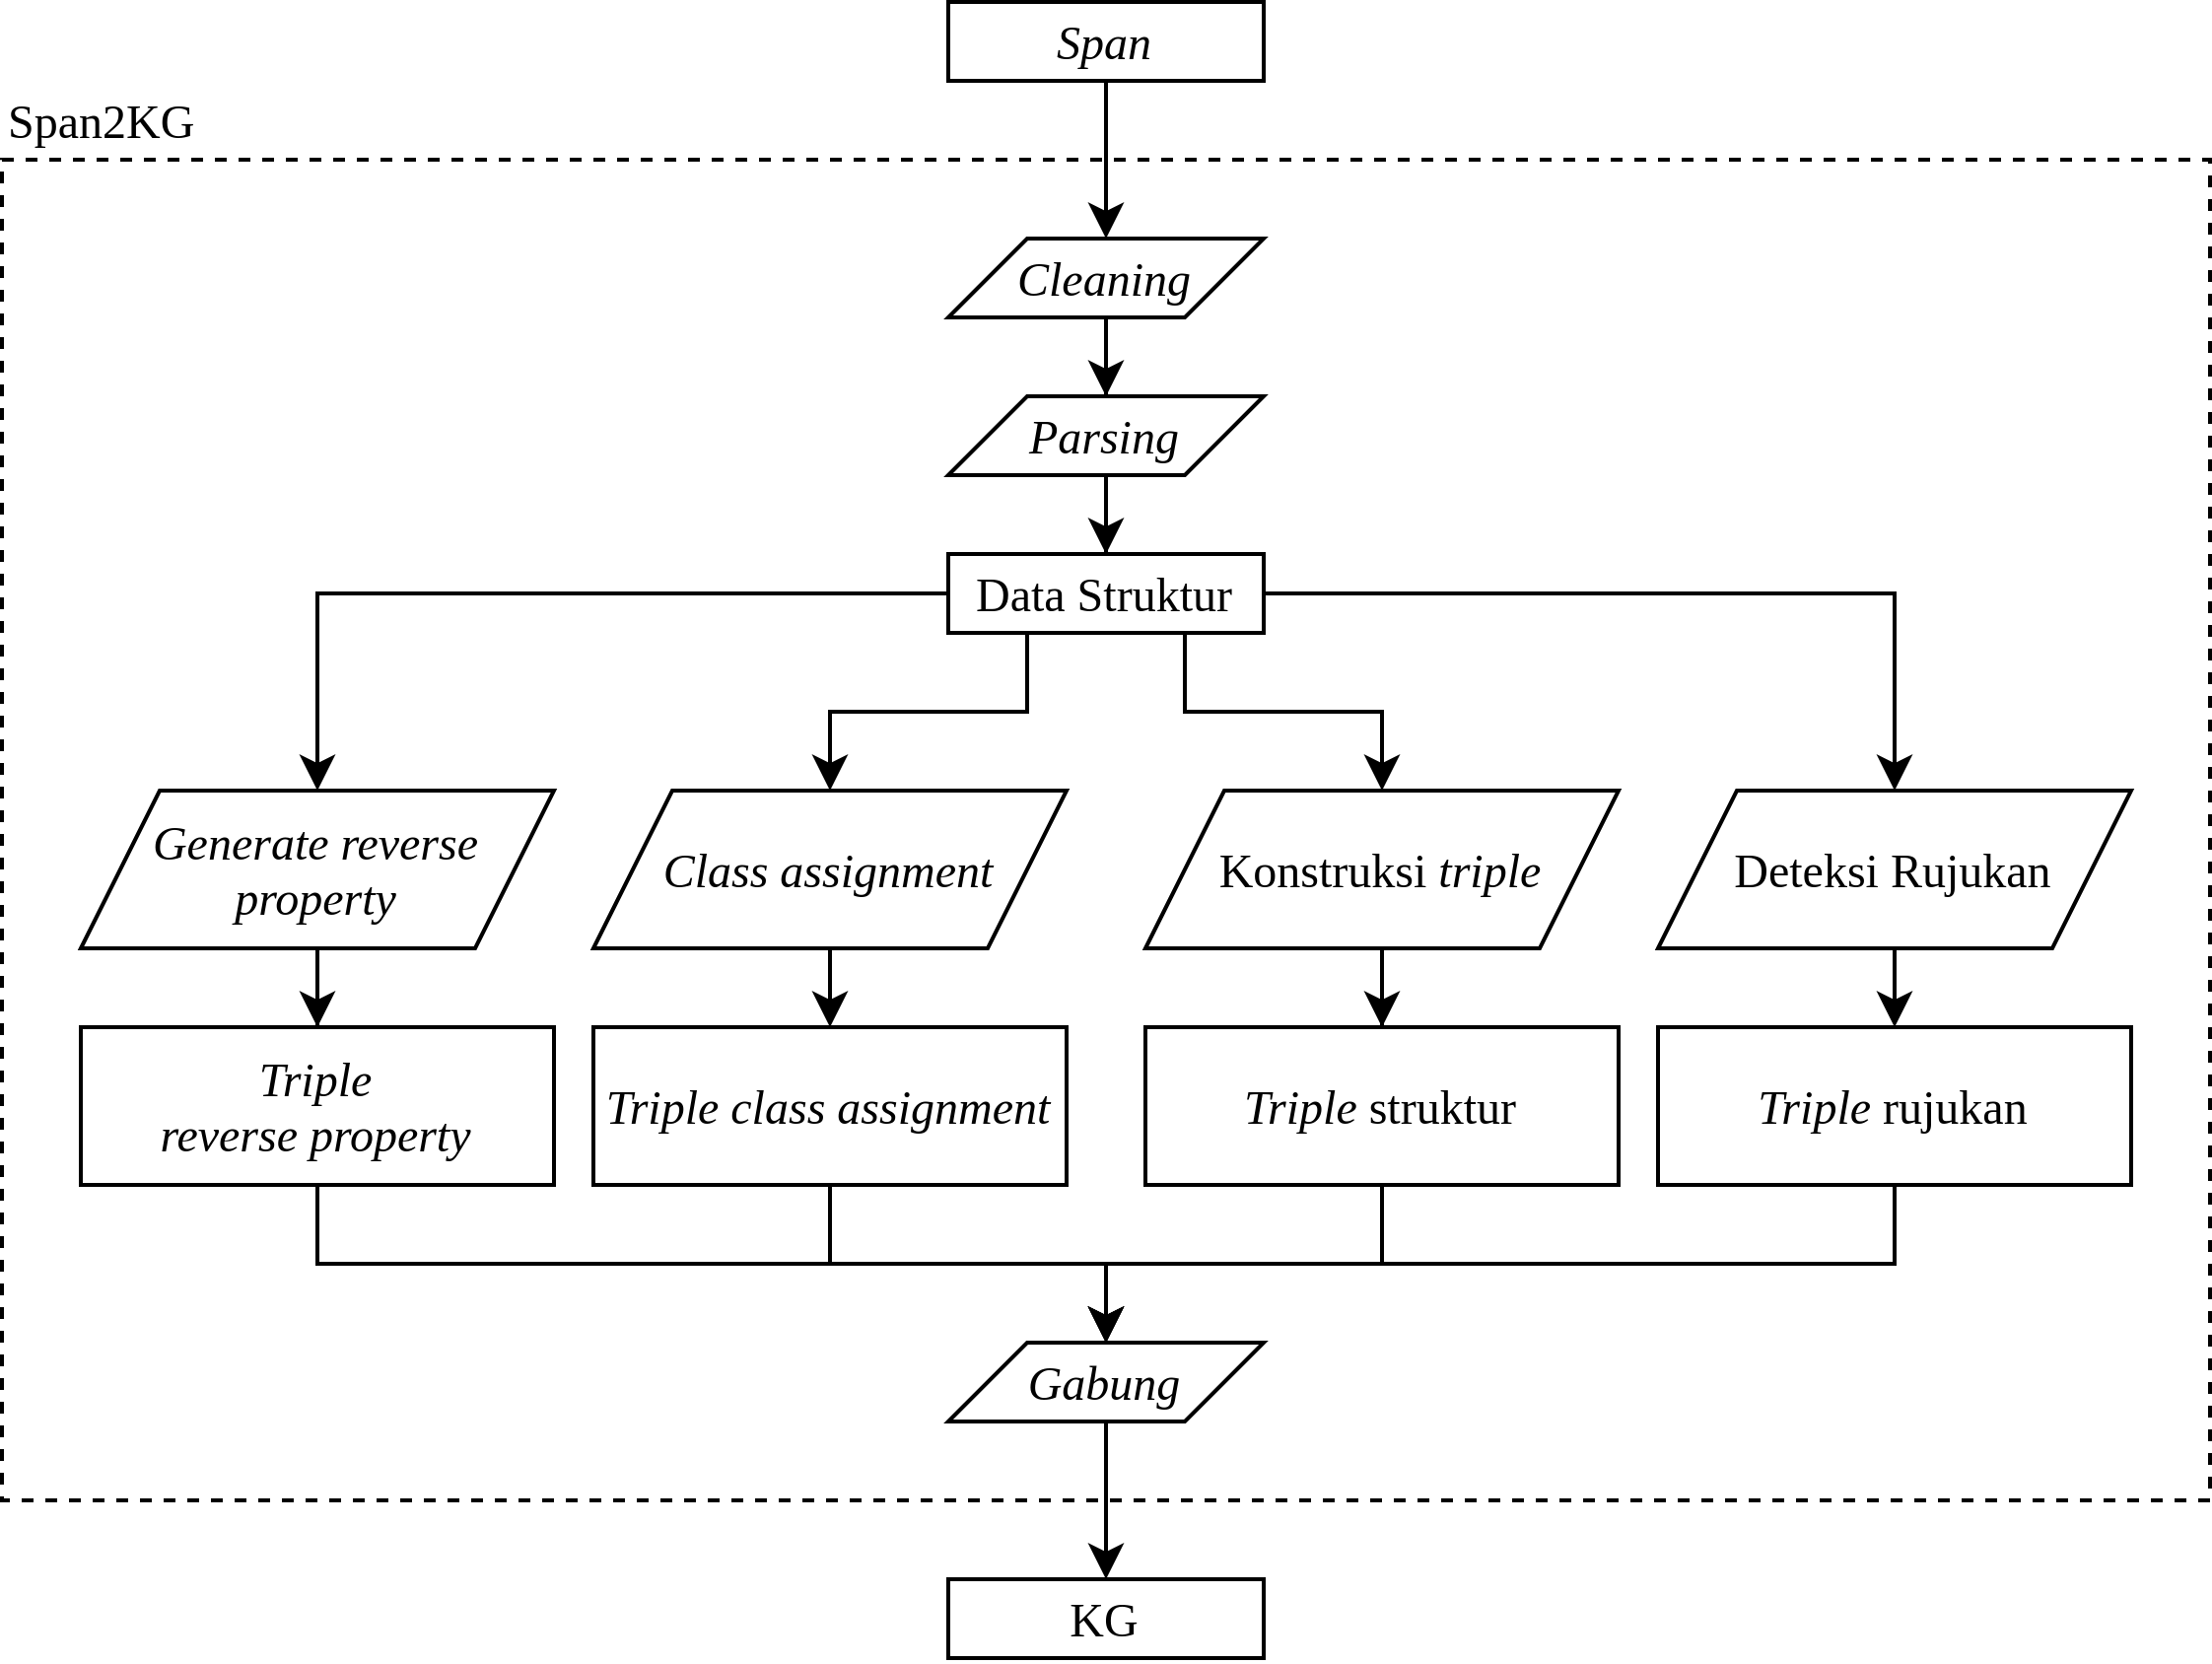
\includegraphics[width=\textwidth]{pictures/span2kg.png}
  \caption{Arsitektur Span2KG}
  \label{fig:span2kg}
\end{figure}

Pada PDF2KG terdapat modul Span2KG yang melakukan konversi \textit{span} menjadi KG dengan
arsitektur seperti yang dijelaskan pada \pic~\ref{fig:span2kg}. Pada Span2KG \textit{span} input
yang terdeteksi sebagai konten yang tidak relevan, seperti \textit{header} dan \textit{footer} yang
berulang, akan disaring. \textit{Clean span} yang dihasilkan, kemudian dilakukan \textit{parsing}
sehingga menjadi data struktur peraturan. Kemudian data tersebut dibuat menjadi \textit{triple}
struktur, \textit{class assignment}, dan \textit{reverse property} sesuai yang didefinisikan pada
ontologi. \textit{Reverse property} merupakan properti yang memiliki sifat kebalikan dari suatu
properti lain, untuk mempermudah \textit{query}. Selain itu, pada data struktur juga dilakukan
deteksi rujukan yang kemudian menghasilkan \textit{triple} rujukan. Pada tahap akhir, Span2KG
menggabungkan semua \textit{triple} tersebut dan dikeluarkan sebagai KG. Pada proses konstruksi KG
ini, \textit{triple} yang dihasilkan akan mengikuti spesifikasi yang diberikan pada ontologi.

%--------------------------------------------------------------------------------------------------%
\section{\textit{Competency Questions}}
\label{sec:competency-questions}
%--------------------------------------------------------------------------------------------------%

\textit{Competency questions} perlu didefinisikan untuk dijadikan landasan perangancan ontologi KG
yang dihasilkan. Setiap \textit{competency question} harus dapat dijawab oleh KG yang dihasilkan
dengan membuktikan SPARQL \textit{query} yang bersesuaian dengan pertanyaan tersebut mengembalikan
hasil yang benar. Pada penelitian ini, \textit{competency questions} disusun dari
pertanyaan-pertanyaan yang menurut peneliti dan dosen pembimbing seharusnya dapat dijawab
berdasarkan informasi yang diberikan pada PDF dari informasi strukturnya, serta data-data yang dapat
diekstrak dengan pemrograman deterministik seperti \textit{regular expression}, bukan seperti
\textit{natural language processing} dan \textit{machine learning}. Beberapa konsep \legal memiliki
konteks spesifik untuk Indonesia, oleh karena itu, pembuatan ontologi akan dilakukan berdasarkan UU
10/2004 tentang pembentukan \legal. \tab~\ref{tab:competency-questions} merupakan daftar
\textit{competency questions} yang didefinisikan pada penelitian ini. Pada \textit{competency
question} terdapat banyak pertanyaan yang terkait dengan UU 11/2020 tentang Cipta Kerja. Hal ini
disebabkan UU Cipta Kerja memuat jenis informasi yang relatif lengkap. Sebagai contoh, UU Cipta
Kerja melakukan ketiga jenis amendemen yaitu penyisipan, pengubahan, dan penghapusan.

\begin{longtable}[l]{|p{0.05\textwidth} | p{0.95\textwidth}|}
  \hline
  \textbf{No.} & \textbf{Pertanyaan}                                                                                                         \\ \hline \endhead
  1            & Deskripsikan UU Cipta Kerja.                                                                                                \\ \hline
  2            & Tampilkan semua pasal dari UU Cipta Kerja.                                                                                  \\ \hline
  3            & Tampilkan teks dari Pasal 2 Ayat 1 UU Cipta Kerja.                                                                          \\ \hline
  4            & Tampilkan semua pasal yang terdapat pada Bab 2 UU Cipta Kerja.                                                              \\ \hline
  5            & Tampilkan ayat yang mengandung teks "kompensasi" dan "buruh" yang disisipkan oleh  UU Cipta Kerja.                          \\ \hline
  6            & Tampilkan komponen dari UU Cipta Kerja yang menyisipkan pasal ke UU Ketenagakerjaan dan pula teks dari pasal tersebut.      \\ \hline
  7            & Tampilkan komponen dari UU Cipta Kerja yang mengubah pasal UU Ketenagakerjaan dan tambilkan sebelum dan setelah pengubahan. \\ \hline
  8            & Tampilkan komponen dari UU Cipta Kerja yang menghapus pasal UU Ketenagakerjaan dan pula teks dari pasal tersebut.           \\ \hline
  9            & Tampilkan peraturan yang paling banyak diamendemen oleh UU Cipta Kerja.                                                     \\ \hline
  10           & Tampilkan banyaknya penyisipan, pengubahan, dan penghapusan pasal yang dilakukan UU Cipta Kerja terhadap UU lain.                 \\ \hline
  11           & Tampilkan pasal pada UU Ketenagakerjaan setelah dilakukan oleh UU Cipta Kerja.                                              \\ \hline
  12           & Tampilkan pasal pada UU Cipta Kerja yang tidak melakukan amendemen.                                                         \\ \hline
  13           & Tampilkan pasal pada UU Cipta Kerja yang menghapus pasal yang disahkan setelah tahun 2001.                                  \\ \hline
  14           & Tampilkan pasal yang disisipkan oleh UU Cipta Kerja dan rujukan yang terdapat pada pasal jika ada.                          \\ \hline
  15           & Tampilkan semua peraturan serta peraturan yang ditimbangnya.                                                                \\ \hline
  16           & Tampilkan 10 peraturan dengan pasal terbanyak.                                                                              \\ \hline
  17           & Tampilkan peraturan yang pernah diamendemen.                                                                                \\ \hline
  18           & Tampilkan 10 tempat terbanyak peraturan disahkan.                                                                           \\ \hline
  19           & Tampilkan 10 peraturan paling banyak ditimbang.                                                                             \\ \hline
  20           & Tampilkan semua peraturan yang melakukan amendemen dan banyaknya pasal yang amendemen oleh pasal tersebut.                  \\ \hline
  21           & Tampilkan jumlah \textit{triple} tentang struktur peraturan.                                                                \\ \hline
  22           & Tampilkan jumlah \textit{triple} tentang metadata peraturan.                                                                \\ \hline
  23           & Tampilkan jumlah \textit{triple} tentang teks peraturan.                                                                    \\ \hline
  24           & Tampilkan jumlah \textit{triple} tentang rujukan peraturan.                                                                 \\ \hline
  25           & Tampilkan jumlah \textit{triple} tentang amendemen peraturan.                                                               \\ \hline
  26           & Tampilkan jumlah \textit{triple} tentang \textit{class assignment}.                                                         \\ \hline
  27           & Tampilkan 5 peraturan dengan komponen terbanyak beserta jumlah komponennya.                                                 \\ \hline
  28           & Peraturan apa yang berlaku pada daerah X yang disahkan di tahun Y?                                                          \\ \hline
  29           & Apa relasi suatu peraturan dengan peraturan lain?                                                                           \\ \hline
  30           & Mana saja peraturan yang membahas tentang topik W atau X tapi bukan topik Y dan bukan Z?                                    \\ \hline
  31           & Apa isi dari Pasal X ayat (Y) huruf Z dari suatu \legal?                                                                    \\ \hline
  32           & Apa saja bab-bab yang terdapat pada peraturan X?                                                                            \\ \hline
  \caption{\textit{Competency questions}}
  \label{tab:competency-questions}
\end{longtable}


%--------------------------------------------------------------------------------------------------%
\section{\textit{Lex2KG Namespace}}
\label{sec:perancangan-uri}
%--------------------------------------------------------------------------------------------------%

Setiap entitas yang berbeda perlu diberikan URI yang berbeda. Penggabungan KG sangat umum dilakukan
karena secara struktur dapat dilakukan dengan mudah, dan dapat memperkuat data dari masing-masing
KG. KG memiliki entitas-entitas dengan URI yang unik, oleh karena itu saat menggabungkan sebuah KG A
dan sebuah KG B, entitas yang berbeda harus memiliki URI yang berbeda. Sebuah masalah dapat terjadi
apabila URI tidak dirancang dengan benar. Sebagai contoh, apabila terdapat entitas dari KG A dengan
URI \mono{https://example.org/trump} dengan maksud Donald Trump mantan presiden Amerika Serikat,
dan entitas dari KG B dengan URI yang sama dengan maksud permainan kartu Trump, saat kedua KG ini
digabung akan menjadi informasi yang berkontradiksi. Oleh karena itu, pada umumnya digunakan
\textit{namespace} yang berbeda untuk masing-masing KG. Sebagai contoh, dengan KG A menggunakan
\textit{namespace} \mono{https://kga.org} dan KG B menggunakan \textit{namespace}
\mono{https://kgb.org}, dua entitas yang sebelumnya berkontradiksi akan memiliki URI yang berbeda
yaitu \mono{https://kga.org/trump} dan \mono{https://kgb.org/trump}.

Pada penelitian ini digunakan \textit{namespace} \mono{https://example.org/lex2kg/}.
\textit{Namespace} yang digunakan oleh Lex2KG dapat dikonfigurasi. \tab~\ref{tab:prefixes} adalah
daftar \textit{prefix} dan notasi singkatnya pada yang akan digunakan pada selanjutnya.

\begin{table}
  \centering
  \begin{tabular}{|l|l|l|} \hline
    notasi singkat & \textit{prefix}                                             \\ \hline \hline
    \texttt{:}     & \texttt{https://example.org/lex2kg/}                        \\ \hline
    \texttt{o:}    & \texttt{https://example.org/lex2kg/ontology/}               \\ \hline
    \texttt{jp:}   & \texttt{https://example.org/lex2kg/ontology/jenisPeraturan} \\ \hline
    \texttt{uu:}   & \texttt{https://example.org/lex2kg/uu/}                     \\ \hline
  \end{tabular}
  \caption{\textit{Prefix} dan notasi singkatnya}
  \label{tab:prefixes}
\end{table}

%--------------------------------------------------------------------------------------------------%
\section{Perancangan \textit{Class} dan URI \textit{Class}}
\label{sec:perancangan-uri-class}
%--------------------------------------------------------------------------------------------------%

Huruf pertama dari nama \textit{class} dibuat kapital mengikuti konvensi RDF \citep{rdf_spec}.
\textit{Class} Lex2KG terdiri dari \textit{Class} komponen \legal seperti \mono{o:Bab} dan
\textit{Class} \legal sendiri yaitu \mono{o:Peraturan}. \tab~\ref{tab:class} adalah semua URI
\textit{class} Lex2KG beserta URI dan deskripsinya.

\begin{longtable}[l]{|p{0.22\textwidth}|p{0.78\textwidth}|}
  \hline
  \textbf{URI Class}        & \textbf{Deskripsi}                                                                              \\ \hline \endhead
  \texttt{o:Peraturan}      & \Legal                                                                                          \\ \hline
  \texttt{o:DaftarBab}      & Daftar satu atau lebih bab                                                                      \\ \hline
  \texttt{o:Bab}            & Bab                                                                                             \\ \hline
  \texttt{o:DaftarBagian}   & Daftar satu atau lebih bagian                                                                   \\ \hline
  \texttt{o:Bagian}         & Bagian                                                                                          \\ \hline
  \texttt{o:DaftarParagraf} & Daftar satu atau lebih paragraf                                                                 \\ \hline
  \texttt{o:Paragraf}       & Paragraf                                                                                        \\ \hline
  \texttt{o:DaftarPasal}    & Daftar satu atau lebih pasal                                                                    \\ \hline
  \texttt{o:Pasal}          & Pasal                                                                                           \\ \hline
  \texttt{o:VersiPasal}     & Versi dari sebuah pasal. Sebuah pasal dapat memiliki satu atau lebih versi dari hasil amendemen \\ \hline
  \texttt{o:DaftarAyat}     & Daftar satu atau lebih ayat                                                                     \\ \hline
  \texttt{o:Ayat}           & Ayat                                                                                            \\ \hline
  \texttt{o:DaftarHuruf}    & Daftar satu atau lebih huruf atau nomor                                                         \\ \hline
  \texttt{o:Huruf}          & Huruf atau nomor                                                                                \\ \hline
  \texttt{o:Menimbang}      & Hal yang ditimbang oleh suatu peraturan                                                         \\ \hline
  \texttt{o:Mengingat}      & Hal yang diingat oleh suatu peraturan                                                           \\ \hline
  \texttt{o:Segmen}         & Segmen teks. Dapat memiliki rujukan ke suatu komponen peraturan                                 \\ \hline
  \caption{Class Lex2KG}
  \label{tab:class}
\end{longtable}

%--------------------------------------------------------------------------------------------------%
\section{Perancangan Jenis Peraturan dan URI Jenis Peraturan}
\label{sec:perancangan-jenis-peraturan}
%--------------------------------------------------------------------------------------------------%

Setiap peraturan memiliki URI yang berbeda, yang akan digunakan oleh entitas sebagai prefix.
\tab~\ref{tab:uri-peraturan} adalah jenis \legal yang diimplementasi pada penelitian ini beserta URI
nya. Variabel akan ditandai dengan kurung kurawal ``\mono{\{\}}''. Diluar jenis peraturan yang
diimplementasi URI nya, ontologi Lex2KG juga memiliki resource sendiri yang mendefinisikan jenis
dari \legal terdaftar pada \tab~\ref{tab:uri-jenis-peraturan}. Beberapa jenis peraturan adalah
spesifik terhadapa kasus di Indonesia, seperti pembagian daerah yurisdiksi dan nama-nama daerah yang
hanya terdapat di Indonesia, sehingga diperlukan perancagan khusus URI untuk kasus Indonesia tersebut.

\begin{longtable}[l]{|p{0.2\textwidth}|p{0.55\textwidth}|p{0.25\textwidth}|}
  \hline
  \textbf{Peraturan}                    & \textbf{URI}                                            & \textbf{Penjelasan variabel}               \\ \hline \endhead
  Undang-Undang Dasar 1945              & \texttt{:uud}                                           &                                            \\ \hline
  Undang-Undang                         & \texttt{:uu/\{thn\}/\{nmr\}}                            & \makecell[l]{\texttt{thn}: tahun peraturan \\\texttt{nmr}: nomor peraturan} \\ \hline
  Peraturan Pemerintah                  & \texttt{:pp/\{thn\}/\{nmr\}}                            & \makecell[l]{\texttt{thn}: tahun peraturan \\\texttt{nmr}: nomor peraturan} \\\hline
  Peraturan Daerah Provinsi DKI Jakarta & \texttt{:perda\_provinsi\_dki\_jakarta/\{thn\}/\{nmr\}} & \makecell[l]{\texttt{thn}: tahun peraturan \\\texttt{nmr}: nomor peraturan} \\\hline
  Peraturan Gubernur DKI Jakarta        & \texttt{:pergub\_dki\_jakarta/\{thn\}/\{nmr\}}          & \makecell[l]{\texttt{thn}: tahun peraturan \\\texttt{nmr}: nomor peraturan} \\\hline
  Peraturan Walikota Malang             & \texttt{:perwali\_malang/\{thn\}/\{nmr\}}               & \makecell[l]{\texttt{thn}: tahun peraturan \\\texttt{nmr}: nomor peraturan} \\\hline
  \caption{Konstruksi URI untuk \legal}
  \label{tab:uri-peraturan}
\end{longtable}

\begin{longtable}[l]{|p{0.5\textwidth}|p{0.5\textwidth}|}
  \hline
  \textbf{Jenis Peraturan}                     & \textbf{URI}                        \\ \hline \endhead
  Undang-Undang Dasar 1945                     & \texttt{jp:UUD}                     \\ \hline
  Ketetapan MPR                                & \texttt{jp:TapMPR}                  \\ \hline
  Undang-Undang                                & \texttt{jp:UU}                      \\ \hline
  Peraturan Pemerintah Pengganti Undang-Undang & \texttt{jp:Perpu}                   \\ \hline
  Peraturan Pemerintah                         & \texttt{jp:PP}                      \\ \hline
  Peraturan Presiden                           & \texttt{jp:Perpres}                 \\ \hline
  Peraturan Menteri                            & \texttt{jp:PeraturanMenteri}        \\ \hline
  Peraturan Daerah Provinsi                    & \texttt{jp:PerdaProvinsi}           \\ \hline
  Peraturan Gubernur                           & \texttt{jp:PeraturanGubernur}       \\ \hline
  Peraturan Daerah Kabupaten/Kota              & \texttt{jp:PerdaKabKota}            \\ \hline
  Peraturan Bupati/Walikota                    & \texttt{jp:PeraturanBupatiWalikota} \\ \hline
  Keputusan Presiden                           & \texttt{jp:KeputusanPresiden}       \\ \hline
  Keputusan Gubernur                           & \texttt{jp:KeputusanGubernur}       \\ \hline
  Keputusan Menteri                            & \texttt{jp:KeputusanMenteri}        \\ \hline
  Keputusan Bupati/Walikota                    & \texttt{jp:KeputusanBupatiWalikota} \\ \hline
  \caption{URI jenis \legal}
  \label{tab:uri-jenis-peraturan}
\end{longtable}

%--------------------------------------------------------------------------------------------------%
\section{Perancangan Komponen dan URI Komponen}
\label{sec:perancangan-komponen}
%--------------------------------------------------------------------------------------------------%

Setiap komponen dokumen merupakan entitas, dan memiliki URI. URI sebuah komponen didahului oleh
\textit{docURI} dan semua komponen yang mengatasinya. \tab~\ref{tab:uri-komponen} adalah jenis
komponen \legal beserta pola URI dan penjelasan variabelnya.

\begin{longtable}{|p{0.22\textwidth}|p{0.33\textwidth}|p{0.45\textwidth}|}
  \hline
  \textbf{Komponen}         & \textbf{URI}                            & \textbf{Penjelasan variabel}                                                                                                                             \\ \hline \endhead
  \texttt{o:DaftarBab}      & \texttt{\{docURI\}/bab}                 & \texttt{docURI}: URI peraturan yang mengatasi                                                                                                            \\ \hline
  \texttt{o:Bab}            & \texttt{\{daftarBabURI\}/\{no\}}        & \texttt{daftarBabURI}: URI \mono{o:DaftarBab} yang mengatasi                                                                                             \\
                            &                                         & \texttt{no}: Nomor bab                                                                                                                                   \\ \hline
  \texttt{o:DaftarBagian}   & \texttt{\{babURI\}/bagian}              & \texttt{babURI}: URI \mono{o:Bab} yang mengatasi                                                                                                         \\ \hline
  \texttt{o:Bagian}         & \texttt{\{daftarBagianURI\}/\{no\}}     & \texttt{daftarBagianURI}: URI \mono{o:DaftarBagian} yang mengatasi                                                                                       \\
                            &                                         & \texttt{no}: Nomor bagian                                                                                                                                \\ \hline
  \texttt{o:DaftarParagraf} & \texttt{\{bagianURI\}/paragraf}         & \texttt{bagianURI}: URI \mono{o:Bagian} yang mengatasi                                                                                                   \\ \hline
  \texttt{o:Paragraf}       & \texttt{\{daftarParagrafURI\}/\{no\}}   & \texttt{daftarParagrafURI}: URI \mono{o:DaftarBagian} yang mengatasi                                                                                     \\
                            &                                         & \texttt{no}: Nomor paragraf                                                                                                                              \\ \hline
  \texttt{o:DaftarPasal}    & \texttt{\{parentURI\}/daftarpasal}      & \texttt{parentURI}: URI \mono{o:Bab}, \mono{o:Bagian}, \mono{o:Paragraf} yang mengatasi                                                                  \\ \hline
  \texttt{o:Pasal}          & \texttt{\{docURI\}/pasal/\{no\}}        & \texttt{docURI}: URI peraturan yang mengatasi                                                                                                            \\
                            &                                         & \texttt{no}: Nomor pasal                                                                                                                                 \\ \hline
  \texttt{o:VersiPasal}     & \texttt{\{pasalURI\}/versi/\{tanggal\}} & \texttt{pasalURI}: URI \mono{o:Pasal} yang mengatasi                                                                                                     \\
                            &                                         & \texttt{tanggal}: Tanggal disahkan                                                                                                                       \\ \hline
  \texttt{o:DaftarAyat}     & \texttt{\{pasalURI\}/ayat}              & \texttt{pasalURI}: URI \mono{o:Pasal} yang mengatasi                                                                                                     \\ \hline
  \texttt{o:Ayat}           & \texttt{\{daftarAyatURI\}/\{no\}}       & \texttt{daftarAyatURI}: URI \mono{o:DaftarAyat} yang mengatasi                                                                                           \\
                            &                                         & \texttt{no}: Nomor ayat                                                                                                                                  \\ \hline
  \texttt{o:DaftarHuruf}    & \texttt{\{parentURI\}/huruf}            & \texttt{parentURI}: URI \mono{o:Ayat}, \mono{o:Huruf}, \mono{o:VersiPasal}, \mono{o:Menimbang}, \mono{o:Mengingat}, yang mengatasi                       \\ \hline
  \texttt{o:Huruf}          & \texttt{\{daftarHurufURI\}/\{id\}}      & \texttt{daftarHurufURI}: URI \mono{o:DaftarHuruf} yang mengatasi                                                                                         \\
                            &                                         & \texttt{id}: Nomor atau huruf                                                                                                                            \\ \hline
  \texttt{o:Menimbang}      & \texttt{\{docURI\}/menimbang}           & \texttt{docURI}: URI peraturan yang mengatasi                                                                                                            \\ \hline
  \texttt{o:Mengingat}      & \texttt{\{docURI\}/mengingat}           & \texttt{docURI}: URI peraturan yang mengatasi                                                                                                            \\ \hline
  \texttt{o:Segmen}         & \texttt{\{parentURI\}/\{name\}}         & \texttt{parentURI}: URI \mono{o:Ayat}, \mono{o:Huruf}, \mono{o:DaftarHuruf}, \mono{o:VersiPasal}, \mono{o:Menimbang}, \texttt{Mengingat}, yang mengatasi \\
                            &                                         & \texttt{name}: Nama teks                                                                                                                                 \\ \hline
  \caption{Konstruksi URI untuk komponen \legal}
  \label{tab:uri-komponen}
\end{longtable}

%--------------------------------------------------------------------------------------------------%
\section{Perancangan Properti dan URI Properti}
\label{sec:perancangan-uri-properti}
%--------------------------------------------------------------------------------------------------%

Properti menghubungkan subjek dan objek. Subjek adalah berupa URI komponen, sedangkan objek dapat
berupa URI komponen, \textit{string}, , atau tanggal. Tipe data atau \textit{class} yang
memungkinkan untuk subjek dari sebuah properti disebut \textit{domain}, sedangkan hal yang sama
untuk objek disebut \textit{range}. \tab~\ref{tab:properti} adalah properti Lex2KG berupa nama,
\textit{domain}, \textit{range}, dan deskripsinya.

\begin{longtable}{|p{0.23\textwidth}|p{0.23\textwidth}|p{0.22\textwidth}|p{0.32\textwidth}|}
  \hline
  \textbf{Nama}              & \textbf{Domain}                                                                                                                  & \textbf{Range}                                        & \textbf{Deskripsi}                                \\ \hline \endhead
  \texttt{o:nomor}           & \texttt{o:Bab}, \texttt{o:Bagian}, \texttt{o:Paragraf}, \texttt{o:Pasal}, \texttt{o:Ayat}, \texttt{o:Huruf}                      & string, bilangan                                      & Nomor atau huruf \_identifier\_ dari komponen     \\ \hline
  \texttt{o:teks}            & \texttt{o:Ayat}, \texttt{o:VersiPasal}, \texttt{o:Segmen}                                                                        & string                                                & teks dari komponen                                \\ \hline
  \texttt{o:bab}             & \texttt{o:DaftarBab}                                                                                                             & \texttt{o:Bab}                                        & Bab                                               \\ \hline
  \texttt{o:bagian}          & \texttt{o:DaftarBagian}                                                                                                          & \texttt{o:Bagian}                                     & Bagian                                            \\ \hline
  \texttt{o:paragraf}        & \texttt{o:DaftarParagraf}                                                                                                        & \texttt{o:Paragraf}                                   & Paragraf                                          \\ \hline
  \texttt{o:pasal}           & \texttt{o:DaftarPasal}                                                                                                           & \texttt{o:Pasal}                                      & Pasal                                             \\ \hline
  \texttt{o:ayat}            & \texttt{o:DaftarAyat}                                                                                                            & \texttt{o:Ayat}                                       & Ayat                                              \\ \hline
  \texttt{o:huruf}           & \texttt{o:DaftarHuruf}                                                                                                           & \texttt{o:Huruf}                                      & Huruf                                             \\ \hline
  \texttt{o:segmen}          & \texttt{o:Mengingat}, \texttt{o:Menimbang}, \texttt{o:Paragraf}, \texttt{o:VersiPasal}, \texttt{o:Huruf}, \texttt{o:DaftarHuruf} & \texttt{o:Segmen}                                     & Segmen                                            \\ \hline
  \texttt{o:daftarBab}       & \texttt{o:Peraturan}                                                                                                             & \texttt{o:DaftarBab}                                  & DaftarBab                                         \\ \hline
  \texttt{o:daftarBagian}    & \texttt{o:Bab}                                                                                                                   & \texttt{o:Daftarbagian}                               & DaftarBagian                                      \\ \hline
  \texttt{o:daftarParagraf}  & \texttt{o:Bagian}                                                                                                                & \texttt{o:DaftarParagraf}                             & DaftarParagraf                                    \\ \hline
  \texttt{o:daftarPasal}     & \texttt{o:Peraturan},\texttt{o:Bab}, \texttt{o:Paragraf}, \texttt{o:Bagian}                                                      & \texttt{o:DaftarPasal}                                & DaftarPasal                                       \\ \hline
  \texttt{o:daftarAyat}      & \texttt{o:VersiPasal}                                                                                                            & \texttt{o:DaftarAyat}                                 & DaftarAyat                                        \\ \hline
  \texttt{o:daftarHuruf}     & \texttt{o:VersiPasal}, \texttt{o:Ayat}, \texttt{o:Huruf}, \texttt{o:Menimbang}, \texttt{o:Mengingat}                             & \texttt{o:DaftarHuruf}                                & DaftarHuruf                                       \\ \hline
  \texttt{o:merujuk}         & \texttt{o:Segmen}                                                                                                                & entitas apapun                                        & Teks merujuk suatu entitas                        \\ \hline
  \texttt{o:mengubah}        & \texttt{o:Huruf}                                                                                                                 & \texttt{o:VersiPasal}                                 & Pengubahan pasal                                  \\ \hline
  \texttt{o:menghapus}       & \texttt{o:Huruf}                                                                                                                 & \texttt{o:VersiPasal}                                 & Penghapusan pasal                                 \\ \hline
  \texttt{o:menyisipkan}     & \texttt{o:Huruf}                                                                                                                 & \texttt{o:VersiPasal}                                 & Penyisipan pasal                                  \\ \hline
  \texttt{o:tanggal}         & \texttt{o:VersiPasal}                                                                                                            & tanggal                                               & Tanggal                                           \\ \hline
  \texttt{o:jenisVersi}      & \texttt{o:VersiPasal}                                                                                                            & 'orisinal', 'penyisipan', 'pengubahan', 'penghapusan' & Jenis versi                                       \\ \hline
  \texttt{o:versi}           & \texttt{o:Pasal}                                                                                                                 & \texttt{o:VersiPasal}                                 & Versi suatu komponen                              \\ \hline
  \texttt{o:tentang}         & \texttt{o:Peraturan}                                                                                                             & string                                                & Peraturan tentang                                 \\ \hline
  \texttt{o:menimbang}       & \texttt{o:Peraturan}                                                                                                             & \texttt{o:Menimbang}                                  & Peraturan menimbang                               \\ \hline
  \texttt{o:mengingat}       & \texttt{o:Peraturan}                                                                                                             & \texttt{o:Mengingat}                                  & Peraturan mengingat                               \\ \hline
  \texttt{o:disahkanPada}    & \texttt{o:Peraturan}                                                                                                             & tanggal                                               & Peraturan disahkan pada tanggal                   \\ \hline
  \texttt{o:disahkanDi}      & \texttt{o:Peraturan}                                                                                                             & string                                                & Peraturan disahkan di lokasi                      \\ \hline
  \texttt{o:disahkanOleh}    & \texttt{o:Peraturan}                                                                                                             & string                                                & Peraturan disahkan oleh                           \\ \hline
  \texttt{o:jabatanPengesah} & \texttt{o:Peraturan}                                                                                                             & string                                                & Jabatan pengesah peraturan                        \\ \hline
  \texttt{o:bagianDari}      & komponen apapun                                                                                                                  & komponen apapun                                       & Komponen subjek adalah bagian dari komponen objek \\ \hline
  \texttt{o:yurisdiksi}      & \texttt{o:Peraturan}                                                                                                             & string                                                & Komponen subjek adalah bagian dari komponen objek \\ \hline
  \texttt{o:jenisPeraturan}  & \texttt{o:Peraturan}                                                                                                             & Jenis Peraturan (\mono{jp:})                          & Komponen subjek adalah bagian dari komponen objek \\ \hline
  \texttt{o:tahun}           & \texttt{o:Peraturan}                                                                                                             & bilangan                                              & Komponen subjek adalah bagian dari komponen objek \\ \hline
  \texttt{o:judul}           & \texttt{o:Bab}, \texttt{o:Bagian}, \texttt{o:Paragraf}                                                                           & string                                                & Komponen subjek adalah bagian dari komponen objek \\ \hline
  \caption{Properti Lex2KG}
  \label{tab:properti}
\end{longtable}

%--------------------------------------------------------------------------------------------------%
\section{Ilustrasi Ontologi}
\label{sec:ilustrasi-ontologi}
%--------------------------------------------------------------------------------------------------%

Untuk memahami ontologi secara intuitif, spesifikasi ontologi pada tabel-tabel diatas dapat
divisualisasikan. \pic~\ref{fig:ontologi-struktur} memuat ontologi struktur dan metadata suatu
\legal. Ontologi struktur adalah berupa komponen-komponen peraturan serta properti yang
menghubungkannya. Ontologi metadata menjelaskan jenis-jenis metadata yang terdapat pada suatu \legal
dan tipe datanya.

\begin{figure}[H]
  \centering
  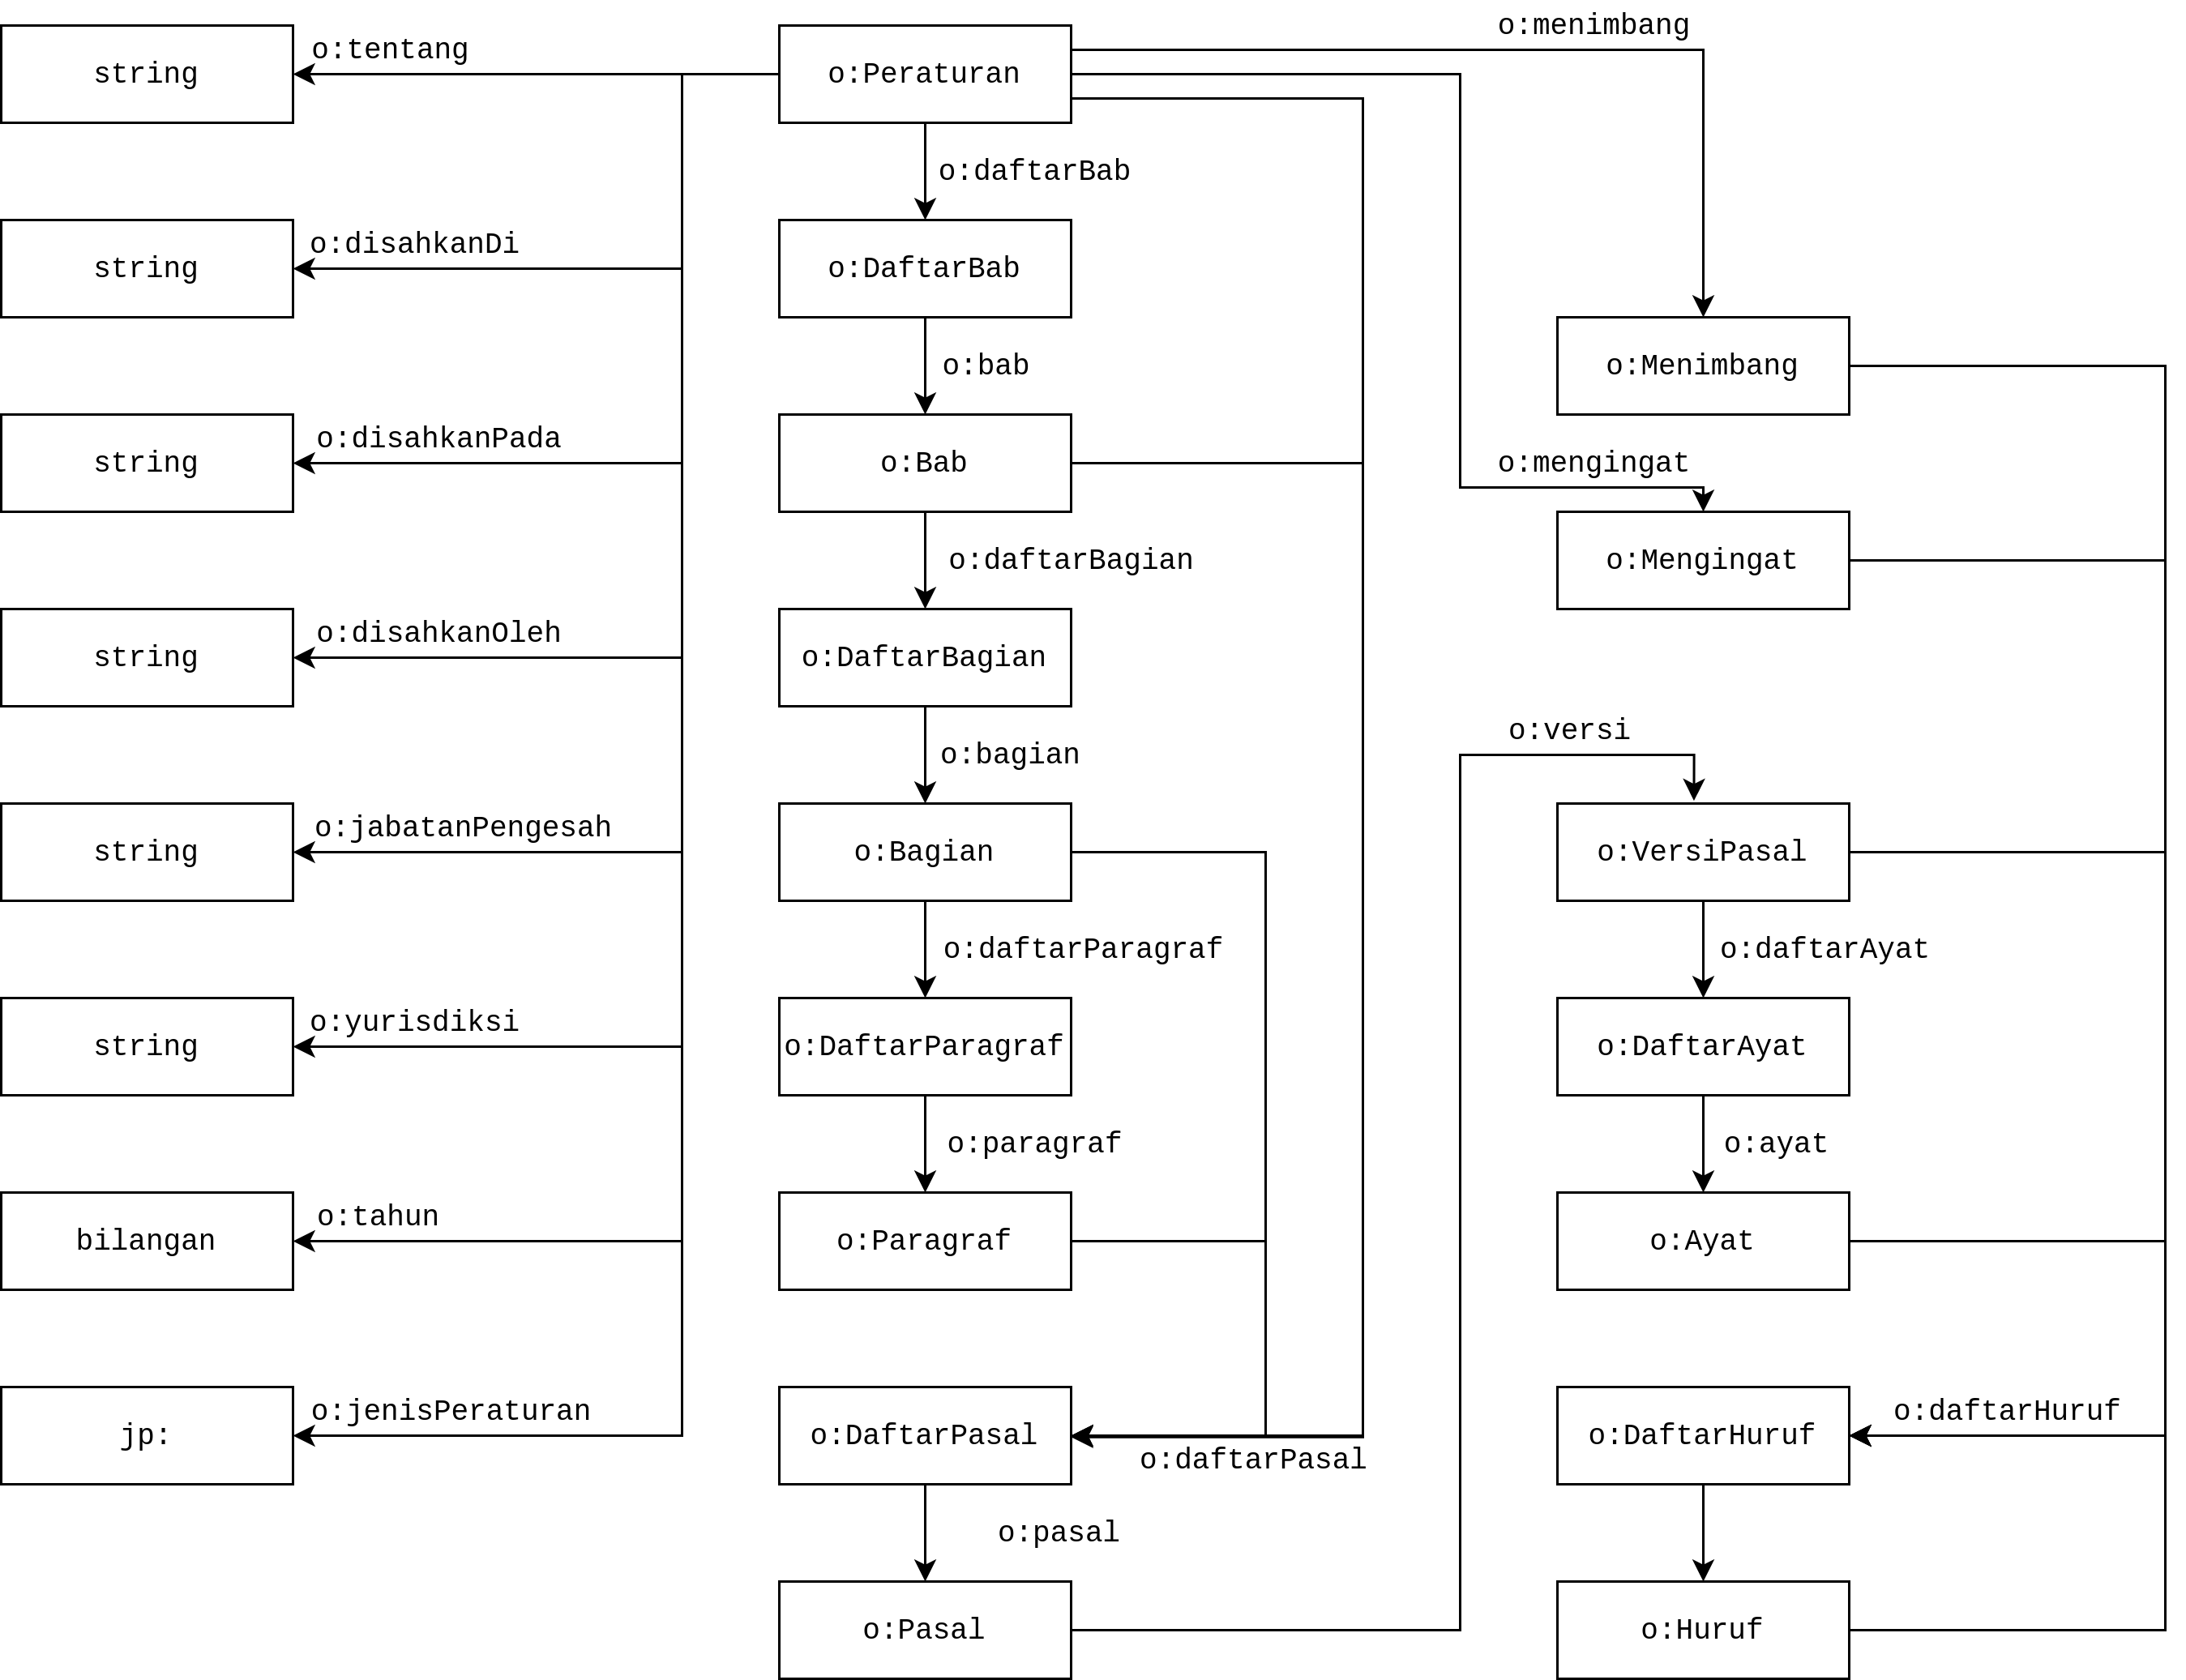
\includegraphics[width=\textwidth]{pictures/ontologi-stuktur.png}
  \caption{Ontology dari metadata dan struktur peraturan}
  \label{fig:ontologi-struktur}
\end{figure}

\pic~\ref{fig:insert}, \pic~\ref{fig:insert}, dan \pic~\ref{fig:insert} memuat ontologi untuk
amendemen peraturan. Setiap terjadi perubahan, akan ditambahkan \mono{VersiPasal} baru. Dengan
ontologi ini, dapat dilakukan \textit{query} untuk mengambil versi terakhir dari pasal untuk dilihat
statusnya apakah orisinal, telah dihapus, hasil pengubahan, atau hasil penyisipan.

\begin{figure}[H]
  \centering
  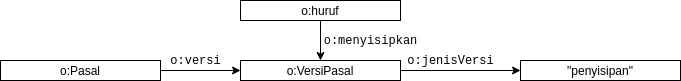
\includegraphics[width=\textwidth]{pictures/insert.png}
  \caption{Ontology penyisipan peraturan}
  \label{fig:insert}
\end{figure}

\begin{figure}[H]
  \centering
  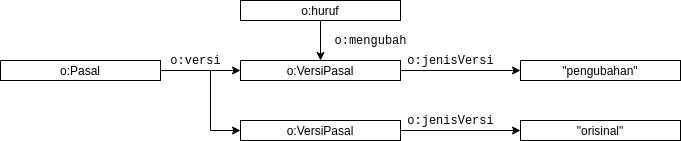
\includegraphics[width=\textwidth]{pictures/update.png}
  \caption{Ontology pengubahan peraturan}
  \label{fig:update}
\end{figure}

\begin{figure}[H]
  \centering
  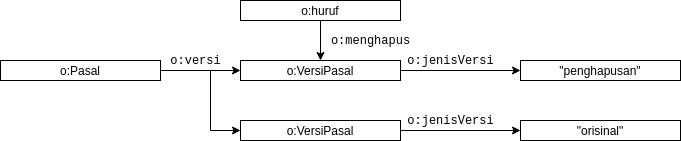
\includegraphics[width=\textwidth]{pictures/delete.png}
  \caption{Ontology penghapusan peraturan}
  \label{fig:delete}
\end{figure}

\clearchapter
%--------------------------------------------------------------------------------------------------%
\chapter{IMPLEMENTASI}
\label{chap:4}
%--------------------------------------------------------------------------------------------------%

Bab ini berisi penjelasan spesifik proses implementasi pada setiap tahap. Secara garis besar
implementasi Lex2KG terdiri dari OCR, pemindaian menjadi \textit{span}, membersihkan \textit{span},
\textit{parsing span} menjadi komponen, deteksi rujukan, dan konstruksi. Selain itu dibahas juga
mengenai bagaimana kualitas konversi dipertahankan dan bagaimana melakukan SPARQL \textit{query}
untuk melakukan evaluasi. Seluruh algoritma dan program yang digunakan dijelaskan secara rinci dalam
bab ini. Seluruh program dan \textit{resource} tersedia pada repositori
Lex2KG.\footnote{\url{https://github.com/aabccd021/legal-kg}}

%--------------------------------------------------------------------------------------------------%
\section{\textit{Maintained PDFs}}
\label{sec:maintained-pdfs}
%--------------------------------------------------------------------------------------------------%

\textit{Maintained PDFs} merupakan berkas-berkas PDF \legal yang akan di-\textit{maintain} kualitas
konversinya. Pengembangan sistem konversi dilakukan secara iteratif, dan setiap terjadi perubahan
pada sistem konversi, akan diperiksa apakah untuk semua \textit{maintained PDFs} memberikan hasil
konversi dengan kualitas yang tinggi. Pemeriksaan hasil konversi dilakukan secara manual dengan
melihat satu per satu \textit{diff} dari hasil konversi. Berikut adalah daftar peraturan
\textit{maintained PDFs}.

\begin{itemize}
  \item Peraturan Daerah Provinsi Jakarta Nomor 2 Tahun 2020 tentang Penanggulangan Corona Virus Disease 2019
  \item Peraturan Gubernur DKI Jakarta Nomor 33 Tahun 2020 tentang Pelaksanaan Pembatasan Sosial Berskala Besar dalam Penanganan Corona Virus Disease 2019 (Covid-19) Di Provinsi Daerah Khusus Ibukota Jakarta
  \item Peraturan Gubernur DKI Jakarta Nomor 3 Tahun 2021 tentang Peraturan Pelaksanaan Peraturan Daerah Nomor 2 Tahun 2020 tentang Penanggulangan Corona Virus Disease 2019
  \item Peraturan Walikota Malang Nomor 19 Tahun 2020 tentang Pedoman Penerapan Masyarakat Produktif dan Aman Covid-19
  \item Peraturan Pemerintah Nomor 74 Tahun 2020 tentang Lembaga Pengelola Investasi
  \item Peraturan Pemerintah Nomor 34 Tahun 2021 tentang Penggunaan Tenaga Kerja Asing
  \item Undang-Undang Nomor 12 Tahun 1997 tentang Perubahan atas Undang-Undang Nomor 6 Tahun 1982 tentang Hak Cipta sebagaimana Telah Diubah dengan Undang-Undang Nomor 7 Tahun 1987
  \item Undang-Undang Nomor 13 Tahun 2003 tentang Ketenagakerjaan
  \item Undang-Undang Nomor 6 Tahun 2018 tentang Kekarantinaan Kesehatan
  \item Undang-Undang Nomor 1 Tahun 2020 tentang Pengesahan Persetujuan Kemitraan Ekomomi
  Komprehensif Indonesia-Australia (Indonesia-Australia Comprehensive Economic Partnership
  Agreement)
  \item Undang-Undang Nomor 11 Tahun 2020 tentang Cipta Kerja
\end{itemize}

%--------------------------------------------------------------------------------------------------%
\section{OCR Ulang Berkas PDF}
\label{sec:ocr-ulang-berkas-pdf}
%--------------------------------------------------------------------------------------------------%

Dokumen \legal yang digunakan pada penelitian didapatkan dalam format berkas PDF. Penulis pada
awalnya mencoba langsung mengekstraksi data dari PDF, tetapi penulis menemukan kesulitan. Salah satu
kesulitan yang penulis temui adalah terdapatnya salah pemindaian pada berkas PDF. Sebagai contoh,
terdapat teks yang tertulis \mono{Pasal} tetapi mengandung data \mono{Pasai}. Selain itu, penulis
juga menemukan bahwa setiap dokumen mengandung keslahan pemindaian yang bervariasi. Untuk suatu
kasus, teks \mono{(2)} selalu terdeteksi sebagai \mono{(21} pada suatu dokumen, tetapi tidak pada
dokumen lainnya. Pada kasus lainnya terdapat dokumen yang hampir tidak memiliki kesalahan pemindaian
dan juga terdapat dokumen yang teksnya tidak dapat dibaca samasekali.

Walaupun dokumen-dokumen tersebut di-\textit{maintain} oleh satu lembaga pada satu situs web, yaitu oleh Dewan
Perwakilan Rakyat pada situs web \url{https://dpr.go.id/jdih}, masing-masing dokumen dibuat menjadi
berkas PDF dengan cara yang berbeda-beda. Penulis tidak dapat mengetahui secara pasti metode apa
yang digunakan, tetapi dari metadata yang didapatkan dari berkas PDF, penulis dapat membuat beberapa
dugaan. Pada berkas PDF, terdapat metadata dengan nama \textbf{Creator}, di mana pada
dokumen-dokumen \legal yang didapatkan, tercantum nama-nama alat pencetak atau
merk dari pencetak tersebut. Dari informasi tersebut penulis menduga bahwa terdapat sebagian
\legal yang dibuat menjadi PDF dengan mencetaknya menjadi kertas terlebih
dahulu kemudian dipindai oleh pemindai dan sebagian lainnya dikonversi langsung dari berkas
\textit{.docx}. Data yang dipindai adalah berupa gambar, artinya teks yang terdapat pada berkas PDF
adalah hasil OCR (\textit{optical character recognition}) oleh pemindai tersebut.
\tab~\ref{tab:metadata-pdf} adalah salah satu contoh dokumen beserta data yang tercantum sebagai
\textbf{Creator} dan contoh kesalahan pemindaiannya yang banyak terjadi.

\begin{table}
  \centering
  \begin{tabular}{|l|l|l|}
    \hline
    Dokumen    & \_\_Creator\_\_        & Kesalahan pemindaian        \\ \hline \hline
    UU 13/2003 & ScanSoft PDF Create! 4 & - (tidak ada)               \\ \hline
    UU 6/2018  & Canon                  & `(2)` selalu dipindai `(21` \\ \hline
    PP 34/2021 & Fuji Xerox B9100       & data teks tidak terbaca     \\ \hline
  \end{tabular}
  \caption{Metadata PDF \legal}
  \label{tab:metadata-pdf}
\end{table}

Pemindaian berkas PDF dengan metode yang berbeda-beda memberikan kualitas hasil pemindaian yang
berbeda-beda dan kesalahan pemindaian yang tidak konsisten. Untuk menyelesaikan masalah ini, penulis
melakukan OCR ulang terhadap semua dokumen yang akan dikonversi. Dengan melakukan OCR ulang
menggunakan satu metode yang sama, penulis tidak hanya berhasil mendapatkan data hasil pemindaian
berkas PDF dengan kualitas pemindaian yang konsisten untuk semua dokumen. Penulis memilih
menggunakan Tesseract OCR\footnote{\url{https://github.com/tesseract-ocr/tesseract}} sebagai metode
OCR karena sifatnya \textit{open source} dan mendukung Bahasa Indonesia sebagai bahasa yang
dipindai. Tesseract OCR merupakan mesin OCR yang awalnya dikembangkan oleh Hewlett-Packard yang
kemudian dibuka sebagai \textit{open source} dan saat ini dilanjutkan pengembangannya oleh Google.
Tesseract OCR juga dianggap \textit{open soure} OCR paling akurat saat ini.

\lst~\ref{lst:run-ocr} merupakan \textit{command} untuk melakukan konversi \mono{UU-2021-34.pdf}
yang sudah ada menjadi \mono{UU-2021-34\_OCR.pdf} hasil OCR. Opsi \mono{--force-ocr} diperlukan
untuk melakukan OCR ulang pada berkas PDF yang sudah memiliki teks hasil OCR untuk di
\textit{overwrite}. Opsi \mono{--jobs 4} menjalankan \textit{command} dengan 4 \textit{core} CPU,
bilangan pada opsi ini dapat diganti sesuai kebutuhan. Opsi \mono{--tesseract-config
tesseract-config.cfg} menjalankan \textit{command} dengan konfigurasi yang diberikan. Pada
penelitian ini, penulis menggunakan Tesseract OCR versi 4.0.

\begin{listing}[H]
  \begin{minted}[fontsize=\scriptsize, frame=single, breaklines]{text}
ocrmypdf -l ind --force-ocr --jobs 4 --tesseract-config tesseract-config.cfg UU-2021-34.pdf
UU-2021-34_OCR.pdf 
  \end{minted}
  \caption{Command untuk menjalankan OCR}
  \label{lst:run-ocr}
\end{listing}

Konfigurasi Tesseract OCR yang digunakan adalah \mono{tessedit\_pageseg\_mode 4} seperti yang
terlihat pada isi file konfigurasi pada \lst~\ref{lst:konfigurasi-ocr}. \mono{tessedit\_pageseg\_mode 4} digunakan agar
Tesseract OCR mendeteksi teks sebagai \textit{block}, bukan \textit{word} atau \textit{character}.

\begin{listing}[H]
  \begin{minted}[fontsize=\scriptsize, frame=single]{text}
# tesseract-config.cfg
tessedit_pageseg_mode 4
  \end{minted}
  \caption{Konfigurasi Tesseract OCR}
  \label{lst:konfigurasi-ocr}
\end{listing}

%--------------------------------------------------------------------------------------------------%
\section{Pemindaian Berkas PDF menjadi \textit{Span}}
\label{pemindaian-berkas-pdf-menjadi-data-span}
%--------------------------------------------------------------------------------------------------%

Agar dapat diproses oleh program, berkas PDF perlu diolah menjadi data berupa daftar teks dan
posisinya yang selanjutnya akan disebut \textit{span}. Sebuah \textit{span} mengandung satu baris
teks. \tab~\ref{tab:data-span} adalah data yang dimiliki oleh sebuah \textit{span}. \textit{Span}
yang dikeluarkan adalah berupa \textit{span} pada masing-masing halaman, sehingga perlu dilakukan
operasi \textit{flatten} untuk menghasilkan array satu dimensi yang memuat \textit{span} dari
seluruh halaman PDF. \pic~\ref{fig:contoh-dokumen} dan \lst~\ref{lst:hasil-pemindaian}
berturut-turut adalah contoh gambaran berkas PDF dan hasil pemindaiannya menjadi daftar
\textit{span}.

\begin{table}
  \centering
  \begin{tabular}{|l|l|} \hline
    Nama             & Deskripsi                                   \\\hline \hline
    \texttt{str}     & teks yand dikandung                         \\\hline
    \texttt{xL}      & koordinat titik terkiri dari \textit{span}  \\\hline
    \texttt{xR}      & koordinat titik terkanan dari \textit{span} \\\hline
    \texttt{y}       & koordinat titik teratas dari \textit{span}  \\\hline
    \texttt{pageNum} & nomor halaman                               \\\hline
    \texttt{id}      & \textit{identifier} unik untuk setiap span  \\\hline
  \end{tabular}
  \caption{Data \textit{span}}
  \label{tab:data-span}
\end{table}

\begin{figure}[H]
  \centering
  \fbox{
\includegraphics{pictures/pdf_example.png}}
  \caption{Contoh PDF yang akan dipindai}
  \label{fig:contoh-dokumen}
\end{figure}

\begin{listing}[H]
  \begin{minted}[fontsize=\scriptsize, frame=single]{yaml}
- xL: 197.52
  xR: 442.79990000000004
  'y': 234.48000000000002
  str: UNDANG-UNDANG REPUBLIK INDONESIA
  pageNum: 1
  id: 0
- xL: 252.72
  xR: 387.6002
  'y': 255.12
  str: NOMOR 13 TAHUN 2003
  pageNum: 1
  id: 1
- xL: 291.12
  xR: 349.68048
  'y': 275.76
  str: TENTANG
  pageNum: 1
  id: 2
- xL: 257.28
  xR: 383.28015999999997
  'y': 296.4
  str: KETENAGAKERJAAN
  pageNum: 1
  id: 3
  \end{minted}
  \caption{Hasil pemindaian \pic~\ref{fig:contoh-dokumen} dalam format yaml}
  \label{lst:hasil-pemindaian}
\end{listing}

%--------------------------------------------------------------------------------------------------%
\section{Membersihkan Data tidak Relevan dari \textit{Span}}
\label{membersihkan-noise-dari-halaman}
%--------------------------------------------------------------------------------------------------%

Tidak jarang dokumen \legal mengandung data tidak relevan yang tidak ingin kita ekstraksi seperti
\textit{header} dan \textit{footer}. Pada penelitian ini, penulis menggunakan dokumen dari sumber
yang sama sehingga memiliki format yang sama, dan juga posisi \textit{header} dan \textit{footer}
yang hampir sama pada setiap dokumen.

\begin{figure}[H]
  \centering
  \fbox{
\includegraphics{pictures/pdf_header.png}}
  \caption{Contoh header}
  \label{fig:contoh-header}
\end{figure}

\pic~\ref{fig:contoh-header} adalah contoh \textit{header} yang terdapat pada setiap halaman. Dapat
dilihat bahwa \textit{header} selalu terdiri dari teks ``PRESIDEN REPUBLIK INDONESIA'' dan diikuti
oleh nomor halaman, dan selalu terletak di posisi yang hampir sama. Oleh karena itu, penulis
memeriksa teks menggunakan \textit{regex} dan posisi dari setiap \textit{span}, kemudian menghapus
\textit{span} tersebut jika terdeteksi sebagai header. \lst~\ref{lst:remove-noise} adalah kode yang
mendeteksi data tidak relevan.

\begin{listing}[H]
  \begin{minted}[fontsize=\scriptsize, fontsize=\scriptsize, frame=single]{typescript}
function isNotHeader(span: UnindexedSpan): boolean {
  const isHeader =
    y < 220 && (['PRESIDEN', 'REPUBLIK INDONESIA'].includes(str) || /- ?[0-9]+ ?-/.test(str));
  return !isHeader;
}
function isLeftFooter(span: UnindexedSpan): boolean {
  return span.y > 900 && span.xL < 45;
}

\end{minted}
  \caption{Kode untuk mendeteksi \textit{header} dan \textit{footer}}
  \label{lst:remove-noise}
\end{listing}

%--------------------------------------------------------------------------------------------------%
\section{Pembuatan \textit{Span} "Hybrid"}
\label{penggabungan-data-berkas-pdf-asli-dan-hasil-ocr-ulang}
%--------------------------------------------------------------------------------------------------%

Pada proses pemindaian berkas PDF menjadi \textit{span}, penulis menemukan satu masalah yaitu data
hasil OCR tidak konsisten dalam memindai angka. Seperti yang dapat dilihat pada
\pic~\ref{fig:contoh-nomor-tidak-terpindai}, angka 10 berhasil dipindai tetapi angka 9 tidak
berhasil. Untuk kasus tersebut, angka hanya tidak terpindai pada hasil OCR, tetapi terpindai dengan
benar pada berkas PDF aslinya. Penulis menggabungkan \textit{span} "Asli" dan \textit{span} "OCR"
untuk membuat \textit{span} "Hybrid" yang melengkapi bagian yang tidak terpindai.

\begin{figure}[H]
  \centering
  \fbox{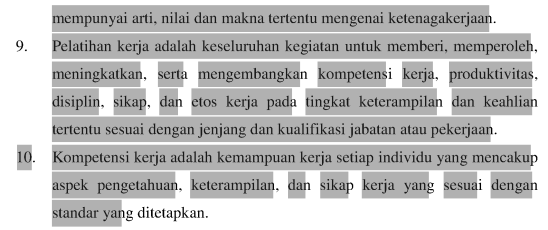
\includegraphics{pictures/pdf_unscanned_number.png}}
  \caption{Contoh nomor tidak terpindai}
  \label{fig:contoh-nomor-tidak-terpindai}
\end{figure}

Penulis hanya melakukan penggabungan \textit{span} untuk kasus angka seperti yang disebutkan di
atas. Hal tersebut dikarenakan pada umumnya kita dapat mentolerir kesalahan pemindaian pada teks,
tetapi karena kegagalan pemindaian pada angka tersebut akan mempengaruhi struktur dokumen, penulis
memutuskan solusi di atas. Sebagai contoh, jika nomor 8 berhasil dipindai dan nomor 9 tidak
berhasil, maka struktur akhir yang dihasilkan akan mengandung semua isi nomor 9 didalam nomor 8,
yang mana seharusnya adalah nomor yang terpisah. \lst~\ref{lst:no-9-tidak-terpindai} dan
\lst~\ref{lst:no-9-terpindai} berturut-turut adalah contoh data yang dihasilkan jika nomor 9 tidak
berhasil terpindai dan jika berhasil terpindai.

\begin{listing}[H]
  \begin{minted}[fontsize=\scriptsize, fontsize=\scriptsize, frame=single]{yaml}
- type: point
  key: 8
  text: >-
    Informasi ketenagakerjaan adalah gabungan, rangkaian, dan analisis data yang
    berbentuk angka yang telah diolah, naskah dan dokumen yang mempunyai arti,
    nilai dan makna tertentu mengenai ketenagakerjaan.
    9. Pelatihan kerja adalah keseluruhan kegiatan untuk memberi, memperoleh,
    meningkatkan, serta mengembangkan kompetensi kerja, produktivitas, disiplin,
    sikap, dan etos kerja pada tingkat keterampilan dan keahlian tertentu sesuai
    dengan jenjang dan kualifikasi jabatan atau pekerjaan.
\end{minted}
  \caption{Data jika nomor 9 tidak berhasil terpindai dalam format yaml}
  \label{lst:no-9-tidak-terpindai}
\end{listing}


\begin{listing}[H]
  \begin{minted}[fontsize=\scriptsize, frame=single]{yaml}
- type: point
  key: 8
  text: >-
    Informasi ketenagakerjaan adalah gabungan, rangkaian, dan analisis data yang
    berbentuk angka yang telah diolah, naskah dan dokumen yang mempunyai arti,
    nilai dan makna tertentu mengenai ketenagakerjaan.
- type: point
  key: 9
  text: >-
    Pelatihan kerja adalah keseluruhan kegiatan untuk memberi, memperoleh,
    meningkatkan, serta mengembangkan kompetensi kerja, produktivitas, disiplin,
    sikap, dan etos kerja pada tingkat keterampilan dan keahlian tertentu sesuai
    dengan jenjang dan kualifikasi jabatan atau pekerjaan.
  
\end{minted}
  \caption{Data jika nomor 9 terpindai dalam format yaml}
  \label{lst:no-9-terpindai}
\end{listing}

%--------------------------------------------------------------------------------------------------%
\section{\textit{Parsing span} menjadi Komponen}
\label{pengelompokan-span-menjadi-komponen}
%--------------------------------------------------------------------------------------------------%

% // TODO: regex2nya bs dtmbhin dan ceritain

Teks yang membentuk suatu komponen terdiri dari satu atau lebih \textit{span}, sehingga daftar
\textit{span} yang didapatkan dari hasil ekstraksi berkas PDF harus dikelompokkan sehingga setiap
kelompok merepresentasikan \textit{span} yang terdapat pada suatu komponen. Pengelompokan dilakukan
dengan mendeteksi \textit{span} awal dan \textit{span} akhir dari sebuah komponen. Karena daftar
\textit{span} hasil ekstraksi bersifat 1 dimensi, hal ini bisa dilakukan dengan melakukan iterasi
pada setiap \textit{span}, kemudian menandai awal atau akhir dari sebuah kelompok apabila memenuhi
suatu pola. Setelah ditandai, \textit{span} akan dikelompokkan sebagai daftar \textit{span} dari
suatu komponen.

Pengelompokan tidak selalu langsung dilakukan dari daftar \textit{span} menjadi komponen. Daftar
\textit{span} dapat dikelompokkan menjadi grup untuk pembagian dokumen secara garis besar, kemudian
baru dikelompokkan sebagai komponen dari masing-masing grup tersebut. Pada
\pic~\ref{fig:ilustrasi-ekstraksi} grup ditandai dengan \textcolor{blue}{warna biru} dan komponen
ditandai dengan \textcolor{red}{warna merah}. Dapat dilihat bahwa daftar \textit{span} data awal
dikelompokkan menjadi komponen \textbf{DaftarBab} dan beberapa grup yaitu \textbf{Judul},
\textbf{Metadata}, dan \textbf{Disahkan}. Kemudian \textit{span} pada grup \textbf{Metadata} dikelompokkan
menjadi komponen \textbf{Menimbang}. Pengelompokan bertingkat ini dilakukan agar fungsi untuk
mendeteksi batas antara komponen tidak menjadi rumit.

\begin{figure}[H]
  \centering
  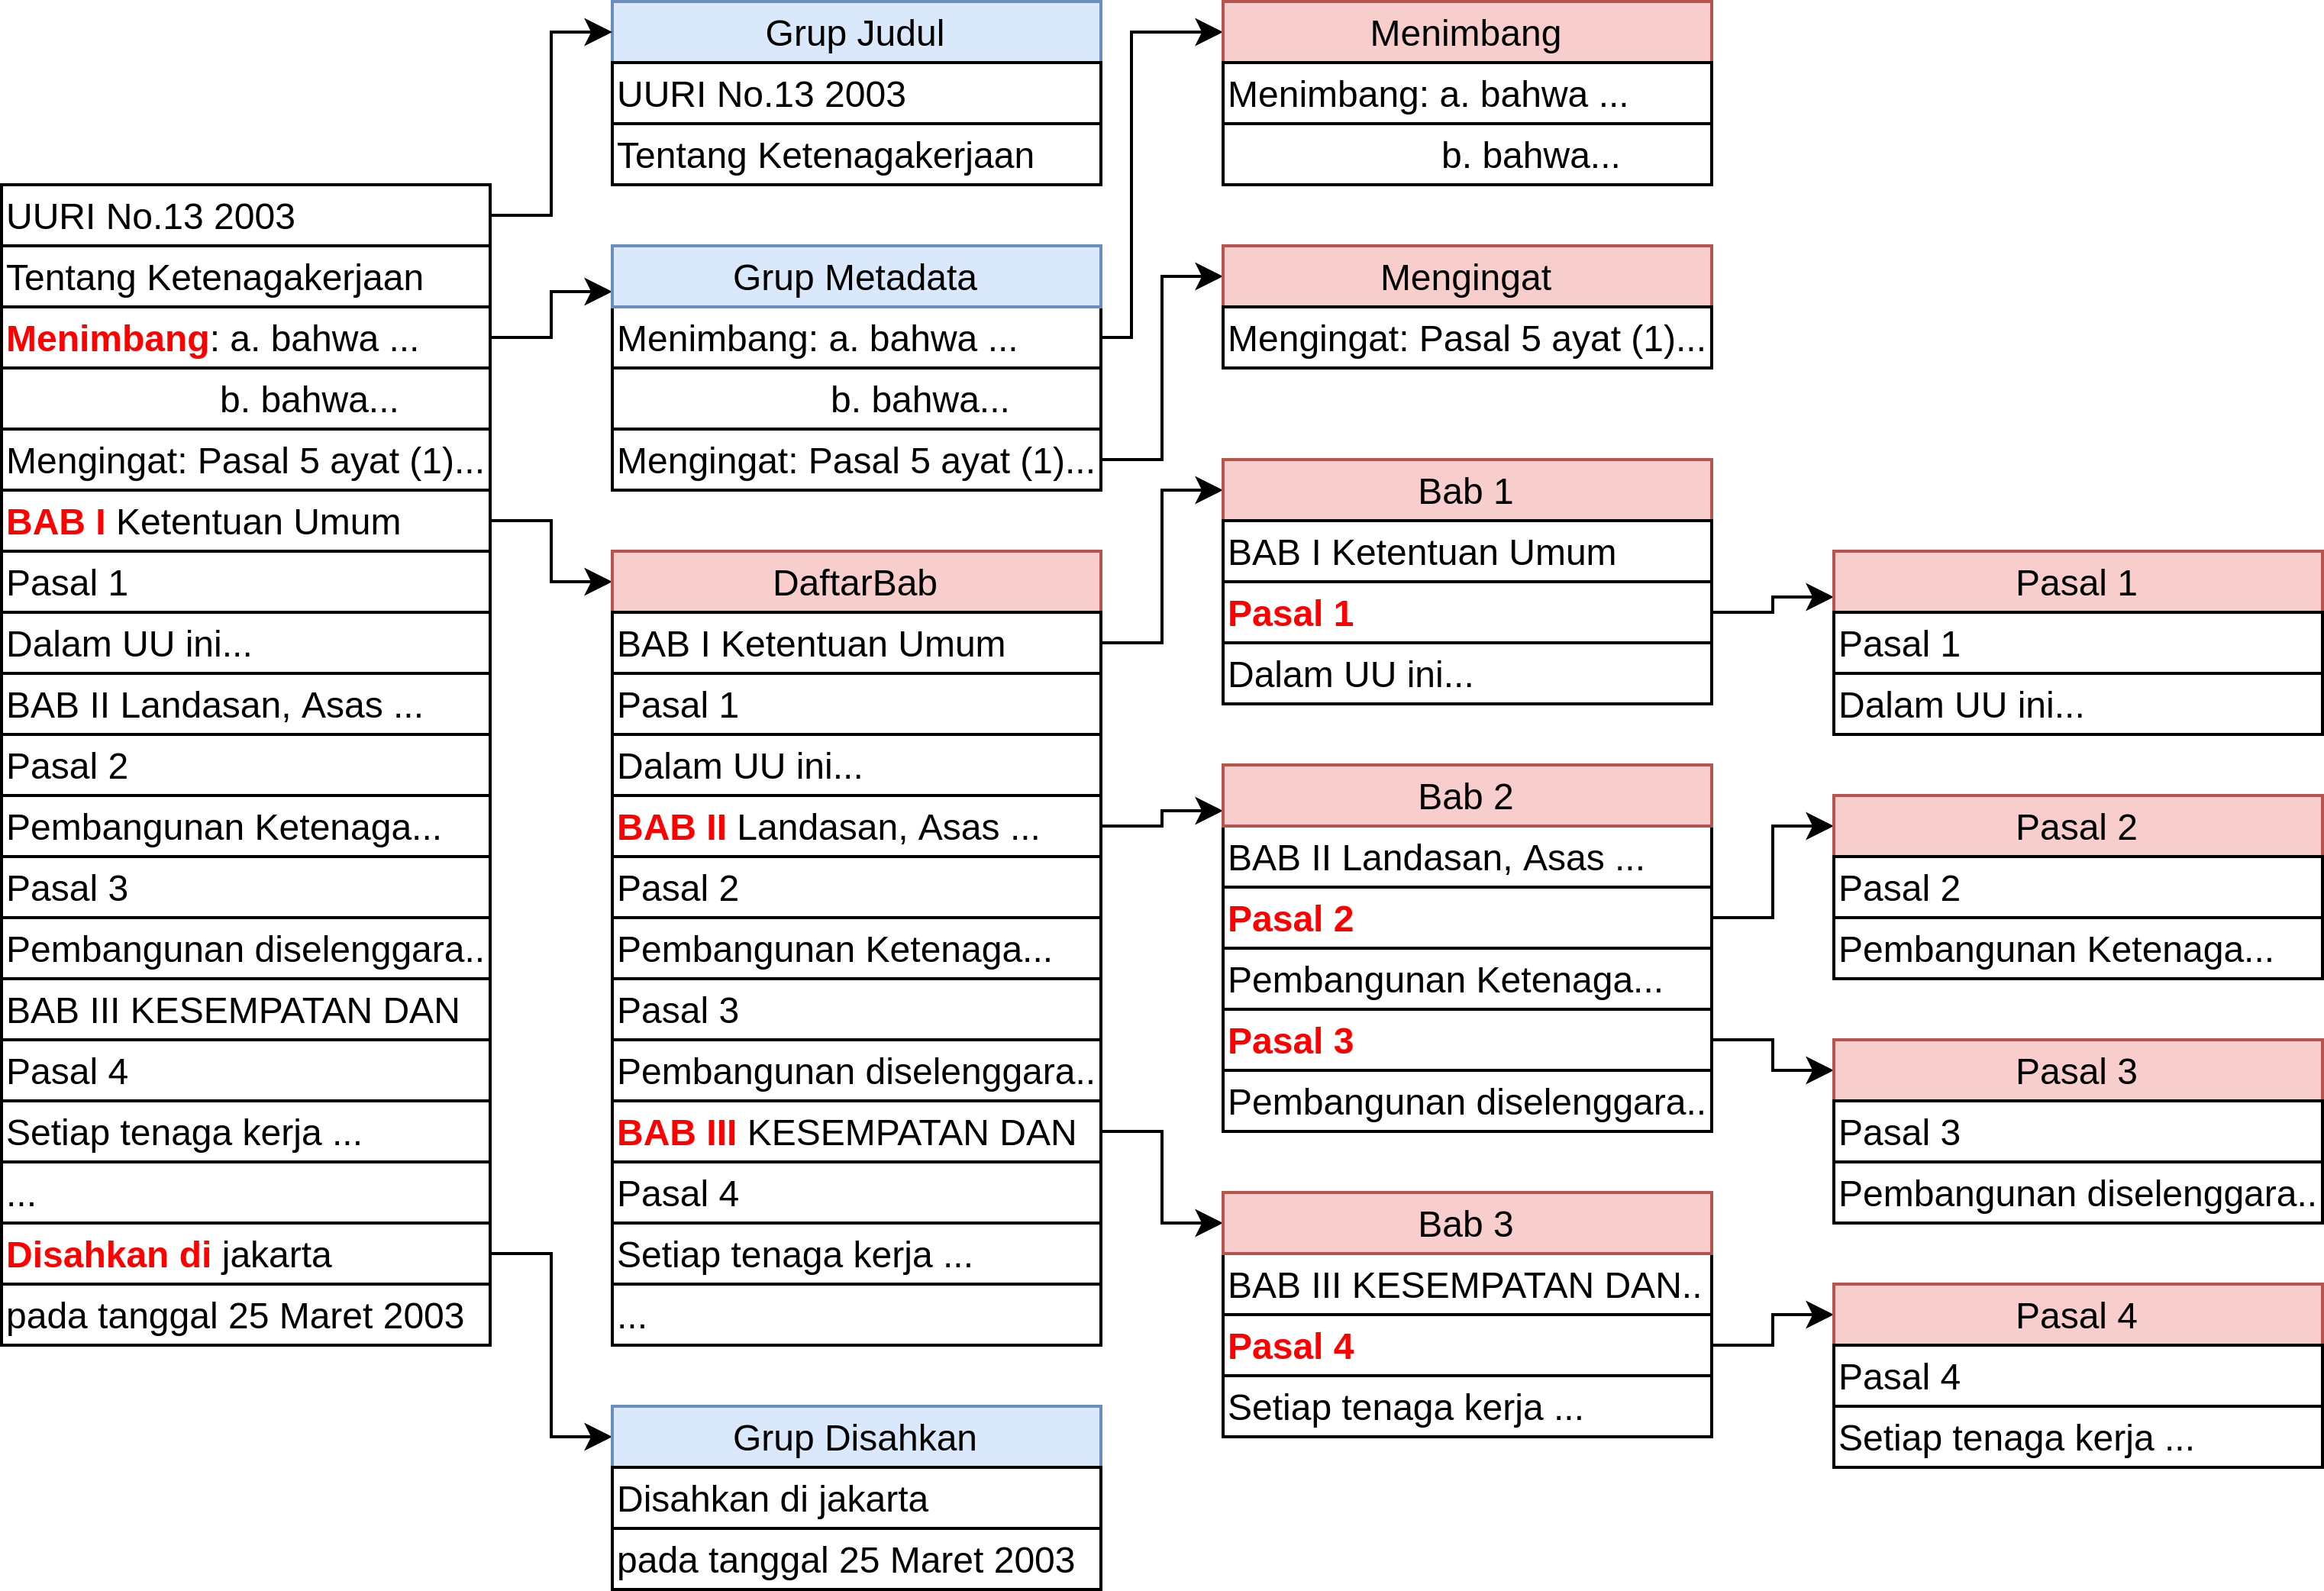
\includegraphics[width=\textwidth]{pictures/pdf_to_component.png}
  \caption{Ilustrasi Ekstraksi Daftar Span menjadi Data Struktur Komponen}
  \label{fig:ilustrasi-ekstraksi}
\end{figure}

Deteksi batas antara komponen atau grup dilakukan dengan melihat data pada \textit{span}
seperti \mono{str}, \mono{xL}, \mono{xR}, dan \mono{y}. Pada \pic~\ref{fig:ilustrasi-ekstraksi},
pola yang terdeteksi sebagai batas ditandai dengan \textcolor{red}{teks merah}. Sebagai contoh, pada
ekstraki paling kiri, dari daftar \textit{span} asli menjadi grup, dilakukan iterasi
\textit{span} dari atas dan akan dimasukkan ke dalam grup \textbf{Judul} sampai menemukan
grup yang diawali dengan kata \mono{Menimbang}. Kemudian setiap \textit{span} setelah
span \textbf{Menimbang} tersebut akan dikelompokkan menjadi grup \textbf{Metadata} sampai
menemukan grup yang diawali kata \mono{BAB I}.

%--------------------------------------------------------------------------------------------------%
\subsection{Komponen Terurut}
\label{subsec:komponen-terurut}
%--------------------------------------------------------------------------------------------------%

Beberapa komponen seperti \mono{o:Bab}, \mono{o:Bagian}, \mono{o:Paragraf}, \mono{o:Pasal}, dan
\mono{o:Huruf} memiliki sifat terurut. Dalam hal ini, yang dimaksud terurut adalah:

\begin{itemize}
  \item Komponen yang mengawali suatu komponen terurut akan selalu sama.
  \item Hanya terdapat satu komponen yang dapat mengikuti komponen terurut.
\end{itemize}

Contoh dari sifat pertama adalah \mono{o:Bab}, \mono{o:Bagian}, \mono{o:Paragraf}, dan
\mono{o:Pasal} pasti dimulai dari komponen nomor 1 seperti \mono{Bab 1} dan \mono{Pasal 1}, dan
\mono{o:Huruf} pasti dimulai dari komponen \mono{a.} atau \mono{1.}. Contoh dari sifat kedua
adalah hanya \mono{pasal 2} yang dapat mengikuti \mono{Pasal 1} dan hanya \mono{b.} yang dapat
mengikuti \mono{a.}. Dalam implementasi, penulis memastikan sifat-sifat ini dipatuhi, sehingga
sebagai contoh apabila sebuah dokumen terdeteksi mengandung \mono{Bab 12} maka akan dijamin
mengandung semua \mono{Bab 1} sampai \mono{Bab 11} dan apabila terdeteksi mengandung
\mono{Pasal 196} maka akan dijamin mengandung semua pasal dari \mono{Pasal 1} sampai
\mono{Pasal 195}.

%--------------------------------------------------------------------------------------------------%
\subsection{Komponen Amendemen}
\label{subsec:komponen-amendemen}
%--------------------------------------------------------------------------------------------------%

Melakukan \textit{parsing span} pada bagian amendemen merupakan salah satu tantangan pada penelitian
ini. \pic~\ref{fig:contoh-amendemen} adalah amendemen pada Pasal 17 UU 11/2020 yang dilakukan
terhadap Pasal 1 UU 26/2007. Dapat dilihat bahwa kata \mono{Pasal 17} dan \mono{Pasal 1} yang
digunakan sebagai pembatas antara komponen memiliki pola teks dan posisi yang hampir sama. Hal ini
membuat pembedaan antara ``Pasal biasa'' dan ``Pasal peng-amendemen'' menjadi sulit dilakukan.

\begin{figure}[H]
  \centering
  \fbox{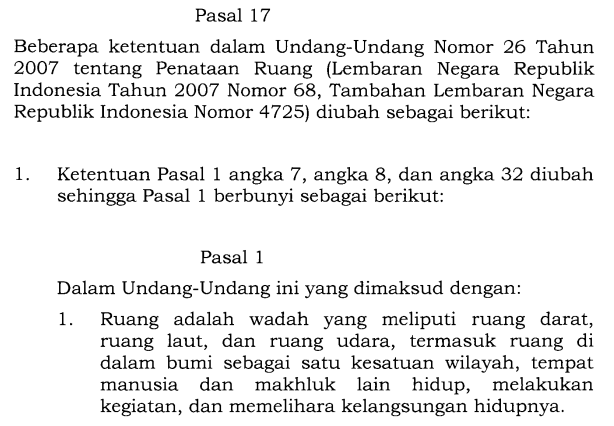
\includegraphics{pictures/pdf_amendment.png}}
  \caption{Contoh Amendemen pada UU 11/2020}
  \label{fig:contoh-amendemen}
\end{figure}

Untuk menyelesaikan masalah ini, penulis menggunakan koordinat \mono{xL} \textit{span} tepat
setelah \textit{span} yang bertuliskan ``Pasal X''. Pada contoh deteksi kompoonen amendemen
\pic~\ref{fig:deteksi-amendemen}, \mono{xL} dari teks setelah pasal peng-amendemen (pasal biasa)
ditandai dengan \textcolor{red}{lingkaran merah}, \mono{xL} dari pasal yang diamendemen ditandai
dengan \textcolor{blue}{lingkaran biru}, dan garis hijau merepresentasikan batas pembeda \mono{xL}
antara pasal biasa dan pasal yang diamendemen. Pembedaan pasal biasa dan pasal amendemen hanya
dilakukan jika dokumen memiliki komponen berupa amendemen.

\begin{figure}[H]
  \centering
  \fbox{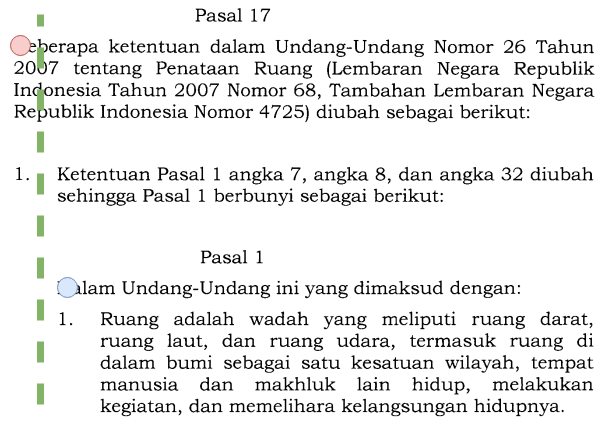
\includegraphics{pictures/amendment_detection.png}}
  \caption{Deteksi Komponen amendemen}
  \label{fig:deteksi-amendemen}
\end{figure}

%--------------------------------------------------------------------------------------------------%
\section{Deteksi Rujukan}
\label{sec:deteksi-rujukan}
%--------------------------------------------------------------------------------------------------%

Setelah semua \textit{span} dikelompokan menjadi suatu komponen, dilakukan deteksi rujukan pada teks
pada setiap komponen untuk mengetahui apakah komponen tersebut menyebut komponen atau dokumen \legal
lainnya. \tab~\ref{tab:rujukan} adalah daftar pola rujukan yang berhasil dideteksi pada penelitian
ini. Selain URI, data rujukan juga mengandung informasi seperti yang dijelaskan pada
\tab~\ref{tab:info-rujukan}. Contoh teks dan data rujukan yang terdeteksi dari teks tersebut dapat
dilihat pada \lst~\ref{lst:uu-13-2003-detect}.

\begin{table}
  \centering
  \begin{tabular}{|l|l|l|} \hline
    No.              & \multicolumn{2}{l|}{}                                                            \\ \hline \hline
    \multirow{4}*{1} & Pola                  & UUD 1945                                                 \\ \cline{2-3}
                     & Regex                 & \verb/Undang Undang Dasar Negara Republik Indonesia Tahun 1945/                               \\ \cline{2-3}
                     & Contoh teks           & Undang Undang Dasar Negara Republik Indonesia Tahun 1945 \\ \cline{2-3}
                     & URI                   & \texttt{:uud}                                            \\ \hline
    \hline
    \multirow{4}*{2} & Pola                  & Undang-Undang Nomor \{x\} Tahun \{y\}                    \\ \cline{2-3}
                     & Regex                 & \verb/Undang-Undang Nomor [0-9]+ Tahun [0-9]+/                               \\ \cline{2-3}
                     & Contoh teks           & Undang-Undang Nomor 26 Tahun 2007                        \\ \cline{2-3}
                     & URI                   & \texttt{:uu/2007/26}                                     \\ \hline
    \hline
    \multirow{4}*{3} & Pola                  & Pasal \{x\}                                              \\ \cline{2-3}
                     & Regex                 & \verb/Pasal [0-9]+/                               \\ \cline{2-3}
                     & Contoh teks           & Pasal 156                                                \\ \cline{2-3}
                     & URI                   & \texttt{:uu/2003/13/pasal/156}                           \\ \hline
    \hline
    \multirow{4}*{4} & Pola                  & ayat (\{x\})                                             \\ \cline{2-3}
                     & Regex                 & \verb/ayat \((l|[0-9]+)\)/                               \\ \cline{2-3}
                     & Contoh teks           & ayat (1)                                                 \\ \cline{2-3}
                     & URI                   & \texttt{:uu/2003/13/pasal/169/ayat/1}                    \\ \hline
    \hline
    \multirow{4}*{5} & Pola                  & Pasal \{x\} ayat (\{x\})                                 \\ \cline{2-3}
                     & Regex                 & \verb/Pasal [0-9]+ ayat \((l|[0-9]+)\)/                               \\ \cline{2-3}
                     & Contoh teks           & Pasal 156 ayat (2)                                       \\ \cline{2-3}
                     & URI                   & \texttt{:uu/2003/13/pasal/156/ayat/2}                    \\ \hline
    \hline
    \multirow{4}*{6} & Pola                  & huruf \{x\} dan huruf \{y\}                              \\ \cline{2-3}
                     & Regex                 & \verb/huruf ?([a-z]?,? ?)+( [a-z]( |,))/                               \\ \cline{2-3}
                     & Contoh teks           & huruf a dan b                                            \\ \cline{2-3}
                     & \multirow{2}*{URI}    & \texttt{uu/2003/13/pasal/1/point/5/point/a}              \\ \cline{3-3}
                     &                       & \texttt{uu/2003/13/pasal/1/point/5/point/b}              \\ \hline
    \hline
    \multirow{4}*{7} & Pola                  & huruf \{x\}, \{y\}, ... dan \{z\}                        \\ \cline{2-3}
                     & Regex                 & \verb/huruf ?([a-z]?,? ?)+( [a-z]( |,))/                               \\ \cline{2-3}
                     & Contoh teks           & huruf a, b, c, d, dan e                                  \\ \cline{2-3}
                     & \multirow{5}*{URI}    & \texttt{uu/2003/13/menimbang/point/a}                    \\ \cline{3-3}
                     &                       & \texttt{uu/2003/13/menimbang/point/b}                    \\ \cline{3-3}
                     &                       & \texttt{uu/2003/13/menimbang/point/c}                    \\ \cline{3-3}
                     &                       & \texttt{uu/2003/13/menimbang/point/d}                    \\ \cline{3-3}
                     &                       & \texttt{uu/2003/13/menimbang/point/e}                    \\ \hline
  \end{tabular}
  \caption{Pola, contoh teks, dan contoh URI deteksi rujukan}
  \label{tab:rujukan}
\end{table}

\begin{table}
  \centering
  \begin{tabular}{|l|l|} \hline
    Nama           & Deskripsi                             \\\hline \hline
    \texttt{start} & \textit{index} karakter awal rujukan  \\\hline
    \texttt{end}   & \textit{index} karakter akhir rujukan \\\hline
    \texttt{uri}   & URI dokumen dan                       \\\hline
  \end{tabular}
  \caption{Data rujukan}
  \label{tab:info-rujukan}
\end{table}

\begin{listing}[H]
  \begin{minted}[fontsize=\scriptsize, frame=single]{yaml}
textString: >-
  Pekerja/buruh yang diputus hubungan kerjanya berdasarkan alasan
  sebagaimana dimaksud dalam ayat (1), dapat memperoleh uang
  penggantian hak sebagaimana dimaksud dalam Pasal 156 ayat (4).
references:
  - start: 91
    end: 99
    uri: /uu/2003/13/pasal/158/ayat/1
  - start: 166
    end: 184
    uri: /uu/2003/13/pasal/156/ayat/4
  \end{minted}
  \caption{Contoh teks pada Pasal 158 Ayat (4) UU 13/2003 beserta rujukan yang terdeteksi}
  \label{lst:uu-13-2003-detect}
\end{listing}

Untuk melakukan deteksi, teks akan melalui fungsi yang masing-masing memiliki pola untuk dideteksi.
Oleh karena itu, untuk \textit{substring} yang beririsan dapat memiliki lebih dari dua rujukan yang
terdeteksi. Pada kasus tersebut akan diambil rujukan dengan \textit{substring} terpanjang. Sebagai
contoh, teks ``Pasal 156 Ayat (4)'' pada UU No.13 Tahun 2003 Pasal 158 Ayat (4) akan terdeteksi
sebagai 3 URI rujukan seperti yang terlihat pada \tab~\ref{tab:contoh-teks-uri}. Pada kasus ini,
yang akan diambil adalah teks ``Pasal 156 ayat (4)'' karena merupakan teks terpanjang.

\begin{table}
  \centering
  \begin{tabular}{|l|l|} \hline
    Teks               & URI                                   \\\hline \hline
    Pasal 156 Ayat (4) & \texttt{/uu/2003/13/pasal/156/ayat/4} \\\hline
    Pasal 156          & \texttt{/uu/2003/13/pasal/156}        \\\hline
    Ayat (4)           & \texttt{/uu/2003/13/pasal/158/ayat/4} \\\hline
  \end{tabular}
  \caption{Contoh teks dan URI yang terdeteksi dari teks tersebut}
  \label{tab:contoh-teks-uri}
\end{table}


%--------------------------------------------------------------------------------------------------%
\section{Konstruksi KG}
\label{data-to-triple}
%--------------------------------------------------------------------------------------------------%

\begin{figure}
  \centering
  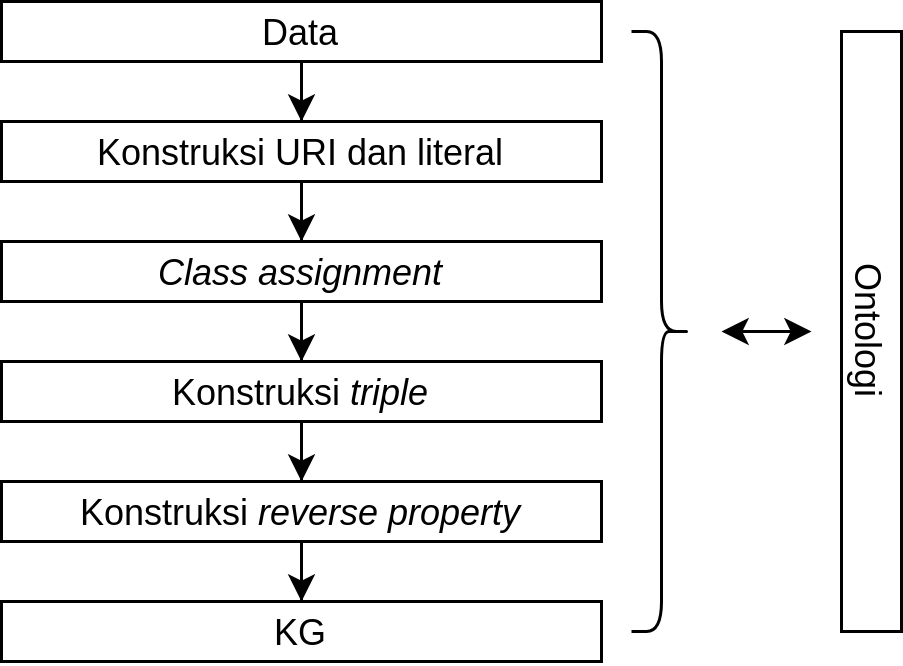
\includegraphics[scale=0.4]{pictures/konstruksi_kg.png}
  \caption{Konstruksi KG}
  \label{fig:konstruksi-kg}
\end{figure}

Seluruh proses konstruksi KG didasari dengan ontologi yang sudah dirancang pada bab sebelumnya. KG
dikonstruksi dari data \legal yang sudah terdapat sebagai data terstruktur dalam memori. Setiap
objek seperti peraturan dan komponen akan dibangun menjadi URI berdasarkan
\tab~\ref{tab:uri-peraturan} dan \tab~\ref{tab:uri-peraturan}. Literal seperti bilangan,
\textit{string}, dan tanggal juga dikonversi sesuai spesifikasi \textit{literal type} pada Turtle.
Setiap objek juga akan di-\textit{assign} ke masing-masing \textit{class} sesuai yang terdapat pada
\tab~\ref{tab:class}. Kemudian \textit{triple} dibangun berdasarkan relasi antara peraturan atau
komponen dengan properti, domain, dan range sesuai spesifikasi pada \tab~\ref{tab:properti}. Untuk
setiap properti struktur, akan dibuat \textit{reverse property} nya yaitu \mono{o:bagianDari}.
Sebagai contoh, jika terdapat \textit{triple} \mono{uu:2020/11/bab o:bab uu:2020/11/bab/1},
\textit{reverse triple} nya adalah \mono{uu:2020/11/bab/1 o:bab uu:2020/11/bab}. Properti struktur
antaralain adalah \mono{o:ayat}, \mono{o:bab}, \mono{o:bagian}, \mono{o:daftarAyat},
\mono{o:daftarBab}, \mono{o:daftarBagian}, \mono{o:daftarHuruf}, \mono{o:daftarParagraf},
\mono{o:daftarPasal}, \mono{o:huruf}, \mono{o:paragraf}, \mono{o:pasal}, \mono{o:segmen},
\mono{o:teks}, dan \mono{o:versi}.


%--------------------------------------------------------------------------------------------------%
\section{Query}
\label{sec:query}
%--------------------------------------------------------------------------------------------------%

\textit{Query} dilakukan terhadap KG untuk evaluasi \textit{competency question} dan membuat
demonstrasi untuk \textit{use case evaluation}. Apache Jena
Fuseki\footnote{\url{https://jena.apache.org/documentation/fuseki2/}} digunakan sebagai SPARQL
server yang menyimpan KG dan melakukan \textit{query} terhadap KG. Di dalam folder Fuseki, Fuseki
dapat dijalankan dengan KG yang memuat berkas Turtle \mono{lex2kg.ttl} dan memiliki endpoint SPARQL
\textit{/lex2kg} dengan \lst~\ref{lst:run-fuseki}. Setelah command tersebut dijalankan, SPARQL
\textit{query} dapat dilakukan menggunakan \textit{client library} dengan endpoint
\url{http://127.0.0.1:3030/lex2kg/sparql}, atau pada antarmuka yang tersedia pada
\url{http://127.0.0.1:3030/dataset.html?tab=query&ds=/lex2kg}. Pada penelitian ini digunakan
\textit{client library}
\texttt{fetch-sparql-endpoint}\footnote{\url{https://www.npmjs.com/package/fetch-sparql-endpoint}}
untuk melakukan \textit{query} dari bahasa pemrograman typescript.


\begin{listing}[H]
  \begin{minted}[fontsize=\scriptsize, frame=single, breaklines]{bash}
java -jar fuseki-server.jar --file=lex2kg.ttl /lex2kg
  \end{minted}
  \caption{Command untuk menjalankan Fuseki}
  \label{lst:run-fuseki}
\end{listing}

%--------------------------------------------------------------------------------------------------%
\section{Konversi Skala Besar}
\label{sec:konversi-skala-besar}
%--------------------------------------------------------------------------------------------------%

Penulis melakukan konversi skala besar pada PDF UU yang terdapat pada Laman Undang-Undang Jaringan
Dokumentasi dan Informasi Hukum DPR RI.\footnote{\url{https://www.dpr.go.id/jdih/uu}} Dari 1669
berkas PDF yang diunduh, 784 diantaranya berhasil dikonversi menjadi KG dengan total 1.163.051
\textit{triple}. Jumlah tripel dikelompokan berdasarkan jenis informasi dapat dilihat pada
\tab~\ref{tab:analisis-triple}. Semua berkas PDF, berkas Turtle hasil konversi, dan berkas
\textit{artifact} seperti PDF hasil OCR, dan \textit{span} dari konversi skala besar dapat diakses
pada repositori \url{https://github.com/aabccd021/uuri}.

\begin{table}
  \centering
  \begin{tabular}{|l|l|} \hline
    Jenis Informasi           & Jumlah Triple \\\hline \hline
    metadata peraturan        & 6.689         \\\hline
    struktur peraturan        & 714.888       \\\hline
    teks                      & 152.301       \\\hline
    rujukan dan amendemen     & 32.577        \\\hline
    \textit{class assignment} & 256.416       \\\hline
  \end{tabular}
  \caption{Analisis \textit{triple} KG hasil konversi skala besar}
  \label{tab:analisis-triple}
\end{table}

%--------------------------------------------------------------------------------------------------%
\section{Hasil Konversi}
\label{sec:hasil-konversi}
%--------------------------------------------------------------------------------------------------%

\lst~\ref{lst:res} merupakan contoh \textit{subset} KG UU 8/2020 tentang Pertanggungjawaban atas
pelaksanaan APBN yang dihasilkan oleh Lex2KG. Dapat dilihat bahwa UU 8/2020 dilengkapi dengan
metadata yang diekstraksi dari PDF, dilengkapi dengan \textit{class assignment} \mono{a
o:Peraturan}, dan diberi jenis peraturan sesuai \textit{resource} pada ontologi yaitu \mono{jp:UU}.
Struktur peraturan berupa menimbang dan teks juga terdapat dalam KG tersebut. \textit{Teverse
property} dari \mono{o:teks} juga dikonstruksi yaitu \mono{o:bagianDari}. \textit{Reverse property}
dari \mono{o:teks} dan \mono{o:huruf} juga dikonstruksi yaitu \mono{o:bagianDari}. Pertimbangan UU
8/2020 terhadap UU 12/2018 juga berhasil diekspresikan daadaplam bentuk rujukan pada komponen
\mono{o:Menimbang}.

\begin{listing}[H]
  \begin{minted}[fontsize=\scriptsize, frame=single, breaklines]{turtle}
@prefix o: <https://example.org/lex2kg/ontology/> .
@prefix jp: <https://example.org/lex2kg/jenisPeraturan/> .

<https://example.org/lex2kg/uu/2020/8>
    a o:Peraturan ;
    o:yurisdiksi "Indonesia";
    o:jenisPeraturan jp:UU;
    o:tahun 2020;
    o:bahasa "id";
    o:tentang " CIPTA KERJA";
    o:disahkanPada "2020-11-02"^^xsd:date;
    o:disahkanDi "Jakarta";
    o:disahkanOleh "JOKO WIDODO";
    o:jabatanPengesah "PRESIDEN REPUBLIK INDONESIA,";
    o:menimbang <https://example.org/lex2kg/uu/2020/8/menimbang> .

<https://example.org/lex2kg/uu/2020/8/menimbang> 
    o:huruf <https://example.org/lex2kg/uu/2020/8/menimbang/huruf/b> .

<https://example.org/lex2kg/uu/2020/8/menimbang/huruf/b> 
    o:bagianDari <https://example.org/lex2kg/uu/2020/8/menimbang> ;
    o:teks <https://example.org/lex2kg/uu/2020/8/menimbang/huruf/b/text> .

<https://example.org/lex2kg/uu/2020/8/menimbang/huruf/b/text> 
    o:bagianDari <https://example.org/lex2kg/uu/2020/8/menimbang/huruf/b> ;
    o:merujuk <https://example.org/lex2kg/uu/2018/12> .

  \end{minted}
  \caption{Contoh KG UU Cipta Kerja}
  \label{lst:res}
\end{listing}


\clearchapter
%--------------------------------------------------------------------------------------------------%
\chapter{EVALUASI}
\label{chap:5}
%--------------------------------------------------------------------------------------------------%

Bab ini berisi evaluasi \textit{use case} KG yang dihasilkan oleh Lex2KG. Evaluasi yang akan
dilakukan adalah berupa SPARQL \textit{query} \textit{chat bot} sederhana, dan visualisasi \legal.
Alasan dari dilakukannya evaluasi kualitatif berupa \textit{use case evaluation} dibanding evaluasi
kuantitatif adalah karena penulis tidak menemukan metode evaluasi kuantitatif yang dapat dilakukan
dengan batasan lingkup penelitian. Sebagai contoh, untuk melakukan evaluasi kualitas KG yang
dihasilkan diperlukan \textit{gold standard} berupa KG yang dibuat oleh manusia dan dijamin benar,
kemudian diukur kualitasnya menggunakan suatu fungsi evaluasi. Membuat KG \textit{gold standard} ini
membutuhkan waktu yang lama, terutama pada kasus penelitian ini di mana ontologi KG nya juga
merupakan bagian penelitian dan dapat berubah dalam jangka waktu penelitian, yang artina
\textit{gold standard} nya juga dapat berubah-rubah.

%--------------------------------------------------------------------------------------------------%
\section{SPARQL Query}
\label{sec:sparq-query}
%--------------------------------------------------------------------------------------------------%

Dengan menggunakan SPARQL server seperi Apache Jena Fuseki, KG yang dibuat dengan Lex2KG dapat
dianalisis dengan menjalankan SPARQL \textit{query}. SPARQL \textit{query} memiliki fitur operasi
\textit{join}, \textit{union}, \textit{optional}, dan \textit{negation pattern}. SPARQL juga
menyediakan \textit{query} analisis yang lengkap seperti \textit{filter}, \textit{aggregate}, dan
\textit{property path}. Semua \textit{competency question} beserta SPARQL \textit{query} yang
menjawab pertanyaan tersebut terdapat pada lampiran. Pada subbab ini akan ditujukan sebaian dari
\textit{query} tersebut untuk dijelaskan fitur SPARQL dan ontologi KG yang digunakan.

%--------------------------------------------------------------------------------------------------%
\subsection{\textit{Query} Amendemen yang Dilakukan UU Cipta Kerja}
\label{subsec:cq8}
%--------------------------------------------------------------------------------------------------%
\textit{Competency question} No. 10 ``Tampilkan banyaknya penyisipan, pengubahan, dan penghapusan
pasal yang dilakukan UU Cipta Kerja terhadap UU lain.'' dapat dijawab dengan melakukan
\textit{query} \lst~\ref{lst:q-10} yang akan memberikan output \tab~\ref{tab:output-q-10}. Pada
\textit{query} digunakan properti \mono{o:menghapus}, \mono{o:menyisipkan}, dan \mono{o:mengubah}
untuk mencari \textit{triple} yang melakukan amendemen. Selain itu digunakan juga fitur SPARQL
\mono{UNION} untuk menggabungkan \textit{triple} dan \mono{BIND} untuk melakukan \textit{assignment}
variabel.

\begin{listing}[H]
  \begin{minted}[fontsize=\scriptsize, frame=single]{sparql}
PREFIX o: <https://example.org/lex2kg/ontology/>

SELECT ?type (COUNT(*) AS ?jumlah) WHERE {
  {
    ?point o:bagianDari+ <https://example.org/lex2kg/uu/2020/11> .
    ?point o:menghapus ?pasal .
    BIND("menghapus" AS ?type)
  } UNION {
    ?point o:bagianDari+ <https://example.org/lex2kg/uu/2020/11> .
    ?point o:menyisipkan ?pasal .
    BIND("menyisipkan" AS ?type)
  } UNION {
    ?point o:bagianDari+ <https://example.org/lex2kg/uu/2020/11> .
    ?point o:mengubah ?pasal .
    BIND("mengubah" AS ?type)
  }
} GROUP BY ?type
LIMIT 3
  \end{minted}
  \caption{SPARQL \textit{query} untuk \textit{competency question} No. 10}
  \label{lst:q-10}
\end{listing}

\begin{table}
  \centering
  \begin{tabular}{|l|r|} \hline
    \texttt{?type} & \texttt{?jumlah} \\\hline \hline
    "menyisipkan"  & 107              \\\hline
    "menghapus"    & 184              \\\hline
    "mengubah"     & 930              \\\hline
  \end{tabular}
  \caption{Output \textit{query} \lst~\ref{lst:q-10} }
  \label{tab:output-q-10}
\end{table}

%--------------------------------------------------------------------------------------------------%
\subsection{\textit{Query} Penimbangan pada Peraturan}
\label{subsec:cq15}
%--------------------------------------------------------------------------------------------------%

\textit{Competency question} No. 15 ``Tampilkan semua peraturan serta peraturan yang ditimbangnya.''
dapat dijawab dengan melakukan \textit{query} \lst~\ref{lst:q-15} yang akan memberikan output
\tab~\ref{tab:output-q-15}. Pada \textit{query} digunakan \mono{o:menimbang} untuk mencari entitas
``menimbang'', \mono{o:bagianDari*} untuk mendapatkan komponen dari entitas ``menimbang''. Selain itu
digunakan juga fitur SPARQL \mono{ORDER BY} yang pada kasus ini dugunakan untuk mengurutkan
\textit{triple} berdasarkan \mono{?penimbang} dan \mono{?ditimbang} secara \textit{descending}.


\begin{listing}[H]
  \begin{minted}[fontsize=\scriptsize, frame=single]{sparql}
PREFIX o: <https://example.org/lex2kg/ontology/>
PREFIX uu: <https://example.org/lex2kg/uu/>

SELECT ?penimbang ?ditimbang
WHERE {
  ?penimbang o:menimbang ?menimbang .
  ?menimbangText o:bagianDari* ?menimbang .
  ?menimbangText o:merujuk ?ditimbang .
  ?ditimbang a o:Peraturan
}
ORDER BY DESC(?penimbang) DESC(?ditimbang)
LIMIT 10

  \end{minted}
  \caption{SPARQL \textit{query} untuk \textit{competency question} No. 15}
  \label{lst:q-15}
\end{listing}

\begin{table}
  \centering
  \begin{tabular}{|l|l|} \hline
    \texttt{?penimbang} & \texttt{?ditimbang} \\\hline \hline
    \texttt{uu:2020/8}  & \texttt{uu:2018/12} \\\hline
    \texttt{uu:2020/6}  & \texttt{uu:2020/2}  \\\hline
    \texttt{uu:2020/6}  & \texttt{uu:2015/1}  \\\hline
    \texttt{uu:2020/6}  & \texttt{uu:2014/1}  \\\hline
    \texttt{uu:2020/2}  & \texttt{uu:2020/1}  \\\hline
  \end{tabular}
  \caption{Output \textit{query} \lst~\ref{lst:q-15} }
  \label{tab:output-q-15}
\end{table}

%--------------------------------------------------------------------------------------------------%
\subsection{\textit{Query} Banyaknya Amendemen Peraturan}
\label{subsec:cq20}
%--------------------------------------------------------------------------------------------------%

\textit{Competency question} No. 20 ``Tampilkan semua peraturan yang melakukan amendemen dan
banyaknya pasal yang amendemen oleh pasal tersebut.'' dapat dijawab dengan melakukan \textit{query}
\lst~\ref{lst:q-20} yang akan memberikan output \tab~\ref{tab:output-q-20}. Selain itu digunakan
juga fitur SPARQL \textit{property path} \mono{|} yang pada kasus ini predikat dapat berupa
\mono{o:mengubah}, \mono{o:menyisipkan}, atau \mono{o:menghapus}

\begin{listing}[H]
  \begin{minted}[fontsize=\scriptsize, frame=single]{sparql}
PREFIX o: <https://example.org/lex2kg/ontology/>
PREFIX uu: <https://example.org/lex2kg/uu/>

SELECT ?doc (COUNT(?point) as ?amendmentCount)
WHERE {
  ?doc a o:Peraturan .
  ?point o:bagianDari* ?doc .
  ?point o:mengubah|o:menyisipkan|o:menghapus ?pasalVersion .
}
GROUP BY (?doc)
ORDER BY DESC(?amendmentCount)
LIMIT 10
  \end{minted}
  \caption{SPARQL \textit{query} untuk \textit{competency question} No. 20}
  \label{lst:q-20}
\end{listing}

\begin{table}
  \centering
  \begin{tabular}{|l|r|} \hline
    \texttt{?doc}       & \texttt{?amandementCount} \\\hline \hline
    \texttt{uu:2020/11} & 1221                      \\\hline
    \texttt{uu:2011/8}  & 20                        \\\hline
    \texttt{uu:2009/26} & 11                        \\\hline
  \end{tabular}
  \caption{Output \textit{query} \lst~\ref{lst:q-20} }
  \label{tab:output-q-20}
\end{table}

%--------------------------------------------------------------------------------------------------%
\section{Visualisasi KG}
\label{sec:visualisasi-kg}
%--------------------------------------------------------------------------------------------------%

Visualisasi data dapat meningkatkan visibilitas dan \textit{explainability} KG. Pada KG dapat
dilakukan visualisasi \textit{node} dan \textit{relation} antara \textit{node}, atau visualisasi
statistik dari KG tersebut. Pada Subbab ini akan diberikan beberapa contoh visualisasi menggunakan
\textit{library} visualisasi VizKG.\footnote{\url{https://pypi.org/project/VizKG/}}

%--------------------------------------------------------------------------------------------------%
\subsection{\textit{Word Cloud} UU Ketenagakerjaan}
\label{subsec:word-cloud}
%--------------------------------------------------------------------------------------------------%

\lst~\ref{lst:vizkg1} merupakan kode untuk melakukan visualisasi \textit{word cloud} dari UU 13/2003
tentang Ketenagakerjaan. Teks yang digunakan untuk \textit{word cloud} diambil dari teks-teks yang
terdapat pada UU 13/2003. Hasil visualisasi pada \pic~\ref{fig:vizkg1} menunjukan bahwa UU ini
paling banyak membicarakan tentang pekerja buruh dan perjanjian kerja.

\begin{listing}[H]
  \begin{minted}[fontsize=\scriptsize, frame=single, breaklines]{python}
sparql_query = """
PREFIX o: <https://example.org/lex2kg/ontology/>
SELECT* WHERE { 
?komponen o:bagianDari* <https://example.org/lex2kg/uu/2003/13> ;
          a o:Segmen ;
          o:teks ?teks .
}
"""
words = vkg(sparql_query=sparql_query, sparql_service_url=sparql_service_url, chart='WordCloud')
words.plot()
  \end{minted}
  \caption{Visualisasi ``Tampilkan 5 peraturan dengan komponen terbanyak beserta jumlah komponennya'' menggunakan VizKG}
  \label{lst:vizkg1}
\end{listing}

\begin{figure}[H]
  \centering
  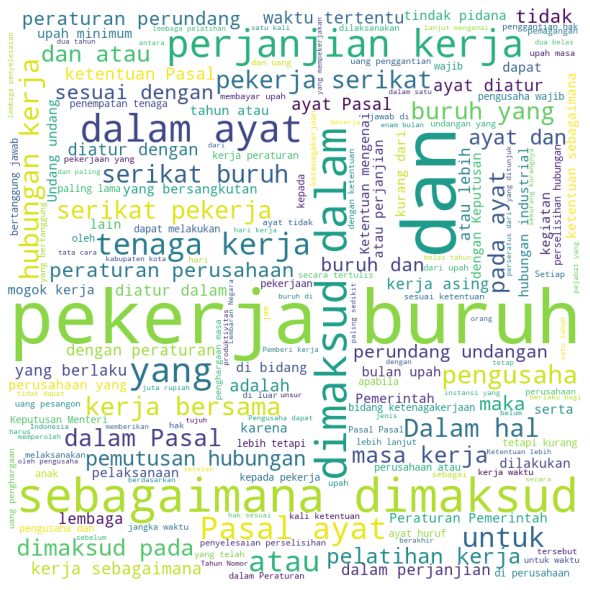
\includegraphics[scale=0.5]{pictures/vizkg1.png}
  \caption{Output VizKG untuk \lst~\ref{lst:vizkg1}}
  \label{fig:vizkg1}
\end{figure}

%--------------------------------------------------------------------------------------------------%
\subsection{Diagram Garis Jumlah UU per Tahun}
\label{subsec:diagram-garis}
%--------------------------------------------------------------------------------------------------%

\lst~\ref{lst:vizkg2} merupakan kode untuk melakukan visualisasi diagram garis jumlah undang-undang
setiap tahunnya. Hasil visualisasi pada \pic~\ref{fig:vizkg2} menunjukan jumlah UU setiap tahunnya
cenderung bertambah. Perlu diperhatikan bahwa UU yang terdapat pada KG hanya UU yang berhasil
dikonversi oleh Lex2KG, oleh sebab itu kecenderungan penambahan jumlah UU bisa jadi disebabkan oleh
kualitas PDF yang makin baik setiap tahunnya.

\begin{listing}[H]
  \begin{minted}[fontsize=\scriptsize, frame=single, breaklines]{python}
sparql_query = """
PREFIX o: <https://example.org/lex2kg/ontology/>
SELECT ?tahun (COUNT(?peraturan) as ?peraturanCount)
WHERE { ?peraturan o:tahun ?tahun .}
GROUP BY ?tahun
ORDER BY ?tahun
"""
words = vkg(sparql_query=sparql_query, sparql_service_url=sparql_service_url, chart='linechart')
words.plot()
  \end{minted}
  \caption{Visualisasi ``Tampilkan 5 peraturan dengan komponen terbanyak beserta jumlah komponennya'' menggunakan VizKG}
  \label{lst:vizkg2}
\end{listing}

\begin{figure}[H]
  \centering
  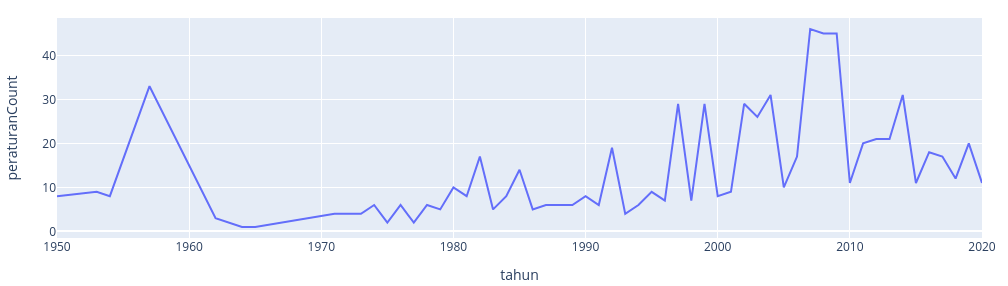
\includegraphics[width=\textwidth]{pictures/vizkg2.png}
  \caption{Output VizKG untuk \lst~\ref{lst:vizkg2}}
  \label{fig:vizkg2}
\end{figure}

%--------------------------------------------------------------------------------------------------%
\subsection{\textit{Graph} ``menimbang''}
\label{subsec:graph}
%--------------------------------------------------------------------------------------------------%

\lst~\ref{lst:vizkg3} merupakan kode untuk melakukan visualisasi \textit{graph} yang menunjukan
hubungan \mono{o:menimbang} antara peraturan, di mana peraturan penimbang disahkan setelah tahun
2017. Hasil visualisasi pada \pic~\ref{fig:vizkg3} bahwa tidak jarang sebuah peraturan ditimbang
oleh atau menimbang lebih dari satu peraturan. Peraturan yang paling banyak ditimbang oleh UU
setelah tahun 2017 adalah UU 24/2000 tentang Perjanjian Internasional.

\begin{listing}[H]
  \begin{minted}[fontsize=\scriptsize, frame=single, breaklines]{python}
sparql_query = """
PREFIX o: <https://example.org/lex2kg/ontology/>
PREFIX uu: <https://example.org/lex2kg/uu/>

SELECT DISTINCT ?penimbang ?penimbangStr ?ditimbang ?ditimbangStr
WHERE {
  ?penimbang o:menimbang ?menimbang .
  ?menimbangText o:bagianDari* ?menimbang .
  ?menimbangText o:merujuk ?ditimbang .
  ?ditimbang a o:Peraturan .
  ?penimbang o:tahun ?tahun .
  BIND(REPLACE(STR(?penimbang),"https://example.org/lex2kg/","") as ?penimbangStr) .
  BIND(REPLACE(STR(?ditimbang),"https://example.org/lex2kg/","") as ?ditimbangStr) .
  FILTER(?tahun > 2017)
}
"""
graph = vkg(sparql_query=sparql_query, sparql_service_url=sparql_service_url, chart="graph")
graph.plot()
  \end{minted}
  \caption{Visualisasi ``Tampilkan 5 peraturan dengan komponen terbanyak beserta jumlah komponennya'' menggunakan VizKG}
  \label{lst:vizkg3}
\end{listing}

\begin{figure}[H]
  \centering
  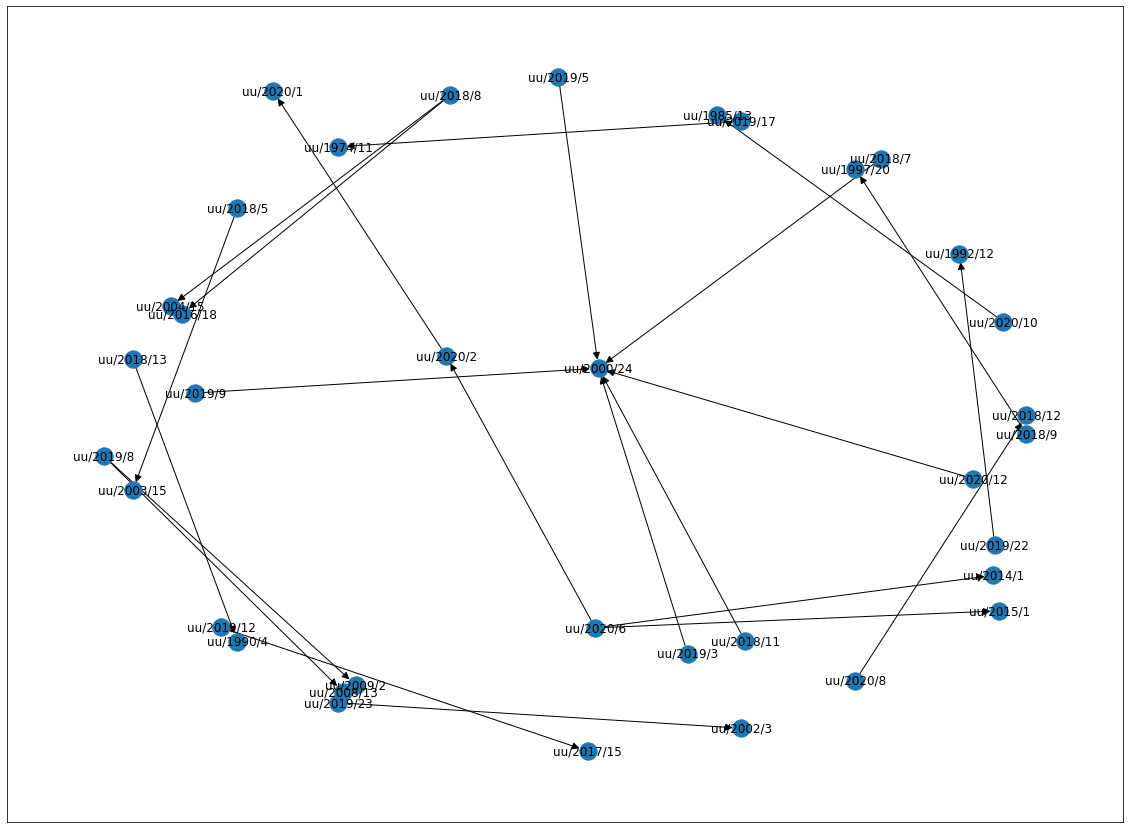
\includegraphics[width=\textwidth]{pictures/vizkg3.png}
  \caption{Output VizKG untuk \lst~\ref{lst:vizkg3}}
  \label{fig:vizkg3}
\end{figure}


%--------------------------------------------------------------------------------------------------%
\section{\textit{Chat bot} sederhana}
\label{sec:chatbot-sederhana}
%--------------------------------------------------------------------------------------------------%

% // HACK: tmbhkn satu skenario yg smpai liat konten

KG \legal dapat digunakan pada \textit{chat bot}. \textit{Chat bot} sederhana memberikan pertanyaan
yang sudah disediakan dan mengembalikan jawaban berdasarkan input pengguna sesuai program
deterministik yang diimplementasi. Pada bab ini akan diperlihatkan bagaimana pengguna melalui
beberapa skenario dan bagaimana \textit{chat bot} nya bekerja. Skenario \textit{chatbot} adalah
sekuensial, artinya Skenario 2 adalah lanjutan dari Skenario 1, dan Skenario 3 adalah lanjutan dari
Skenario 2. Input pengguna akan digunakan sebagai input dari template SPARQL \textit{query} yang
sudah tersedia. Teks yang ditampilkan \textit{chat bot} ditandai dengan warna hitam, dan teks input
pengguna ditandai dengan \textcolor{red}{warna merah}.

%--------------------------------------------------------------------------------------------------%
\subsection{Skenario 1: Mencari Peraturan dengan Kata Kunci}
\label{subsec:skenario-1}
%--------------------------------------------------------------------------------------------------%

\lst~\ref{lst:chatbot-1} merupakan tampilan chatbot pada Skenario 1 di mana pengguna dapat mencari
\legal dengan kata kunci tertentu. Pada contoh ini pengguna mencari peraturan dengan kata kunci
``kerja'', kemudian \textit{chat bot} melakukan \textit{query} terhadap KG menggunakan template
\lst~\ref{lst:chatbot-1-query}, di mana \mono{inputStr} memiliki nilai ``kerja''. Kemudian
\textit{chat bot} mengembalikan hasil \textit{query} berupa nama \legal yang pada judulnya terdapa
\textit{substring} kerja.

\begin{listing}[H]
  \begin{center}
    \begin{tabular}{|p{0.9\textwidth}|}
      \hline
      \makecell[l]{
        \texttt{Masukkan Kata Kunci Peraturan: \textcolor{red}{kerja}}    \\ \\
        \texttt{Berikut adalah peraturan yang judulnya mengandung kerja.} \\
        \texttt{Pilih salah satu untuk melihat lebih lanjut.}             \\
        \texttt{uu/2004/17}                                               \\
        \texttt{uu/2016/3}                                                \\
        \texttt{uu/1997/25}                                               \\
        \texttt{uu/2016/15}                                               \\
        \texttt{uu/2007/47}                                               \\
        \texttt{uu/1991/1}                                                \\
        \texttt{uu/2019/3}                                                \\ \\
        \texttt{Pilih salah satu untuk melihat lebih lanjut: }
      }                                                                   \\
      \hline
    \end{tabular}
  \end{center}
  \caption{Tampilan \textit{chat bot} untuk Skenario 1}
  \label{lst:chatbot-1}
\end{listing}

\begin{listing}[H]
  \begin{minted}[fontsize=\scriptsize, frame=single]{typescript}
    const res = await sparqlQuery({
      queryStr: `
PREFIX o: <https://example.org/lex2kg/ontology/>
SELECT ?doc ?title
WHERE {
  ?doc a o:Peraturan .
  ?doc o:tentang ?title.
  FILTER REGEX(STR(?title), "${inputStr.toUpperCase()}")
}
`,
    });
  \end{minted}
  \caption{\textit{Query} template untuk Skenario 1}
  \label{lst:chatbot-1-query}
\end{listing}

%--------------------------------------------------------------------------------------------------%
\subsection{Skenario 2: Menampilkan Metadata Peraturan}
\label{subsec:skenario-2}
%--------------------------------------------------------------------------------------------------%

\lst~\ref{lst:chatbot-2} merupakan tampilan chatbot pada Skenario 2 di mana pengguna memilih
peraturan berdasarkan pilihan yang diberikan sebelumnya, kemudian menampilkan metadatanya. Pada
contoh ini pengguna memilih peraturan \mono{uu/2019/3} dan data\mono{metadata}, kemudian
\textit{chat bot} melakukan \textit{query} terhadap KG menggunakan template
\lst~\ref{lst:chatbot-2-query}, di mana \mono{legalURI} memiliki nilai \mono{uu/2019/3}. Kemudian
\textit{chat bot} mengembalikan hasil \textit{query} berupa metadata UU 3/2019.

\begin{listing}[H]
  \begin{center}
    \begin{tabular}{|p{0.9\textwidth}|}
      \hline
      \makecell[l]{
        \texttt{Pilih salah satu untuk melihat lebih lanjut: \textcolor{red}{uu/2019/3}} \\
        \\
        \texttt{Data uu/2019/3 :}                                                        \\
        \texttt{-metadata}                                                               \\
        \texttt{-menimbang}                                                              \\
        \texttt{-konten}                                                                 \\
        \\
        \texttt{Pilih data yang ingin anda lihat: \textcolor{red}{metadata}}             \\
        \\
        \texttt{yurisdiksi: Indonesia}                                                   \\
        \texttt{jenisPeraturan: UU}                                                      \\
        \texttt{tahun: 2019}                                                             \\
        \texttt{bahasa: id}                                                              \\
        \texttt{tentang:  PENGESAHAN NOTA KESEPAHAMAN ANTARA PEMERINTAH REPUBLIK...}     \\
        \texttt{disahkanPada: 2009-01-10}                                                \\
        \texttt{disahkanDi: Jakarta}                                                     \\
        \texttt{disahkanOleh: JOKO WIDODO}                                               \\
        \texttt{jabatanPengesah: PRESIDEN REPUBLIK INDONESIA,}                           \\
        \\
        \texttt{Pilih data yang ingin anda lihat:}
      }                                                                                  \\
      \hline
    \end{tabular}
  \end{center}
  \caption{Tampilan \textit{chat bot} untuk Skenario 2}
  \label{lst:chatbot-2}
\end{listing}



\begin{listing}[H]
  \begin{minted}[fontsize=\scriptsize, frame=single, breaklines]{typescript}
    const res = await sparqlQuery({
      queryStr: `
PREFIX o: <https://example.org/lex2kg/ontology/>
SELECT ?label ?data
WHERE {
<https://example.org/lex2kg/${legalURI}> o:yurisdiksi| o:jenisPeraturan| o:tahun| o:bahasa| o:tentang| o:disahkanPada| o:disahkanDi| o:disahkanOleh| o:jabatanPengesah ?data ;
    ?label ?data .
}
`,
    });
  \end{minted}
  \caption{\textit{Query} template untuk Skenario 2}
  \label{lst:chatbot-2-query}
\end{listing}

%--------------------------------------------------------------------------------------------------%
\subsection{Skenario 3: Melihat Peraturan yang ditimbang oleh Peraturan}
\label{subsec:skenario-3}
%--------------------------------------------------------------------------------------------------%

\lst~\ref{lst:chatbot-3} merupakan tampilan chatbot pada Skenario 3 di mana pengguna memilih
peraturan berdasarkan pilihan yang diberikan sebelumnya, kemudian menampilkan peraturan yang
ditimbangnya. Pada contoh ini pengguna memilih \mono{menimbang} untuk informasi yang ingin
ditampilkan, kemudian \textit{chat bot} melakukan \textit{query} terhadap KG menggunakan template
\lst~\ref{lst:chatbot-3-query}, di mana \mono{legalURI} memiliki nilai \mono{uu/2019/3}. Kemudian
\textit{chat bot} mengembalikan hasil \textit{query} berupa dokumen yang ditimbang UU 3/2019 yaitu
UU 24/2000.

\begin{listing}[H]
  \begin{center}
    \begin{tabular}{|p{0.9\textwidth}|}
      \hline
      \makecell[l]{
        \texttt{Data uu/2019/3 :}                                             \\
        \texttt{-metadata}                                                    \\
        \texttt{-menimbang}                                                   \\
        \texttt{-konten}                                                      \\
        \\
        \texttt{Pilih data yang ingin anda lihat: \textcolor{red}{menimbang}} \\
        \\
        \texttt{uu/2000/24}
      }                                                                       \\
      \hline
    \end{tabular}
  \end{center}
  \caption{Tampilan \textit{chat bot} untuk Skenario 3}
  \label{lst:chatbot-3}
\end{listing}

\begin{listing}[H]
  \begin{minted}[fontsize=\scriptsize, frame=single, breaklines]{typescript}
    const res = await sparqlQuery({
      queryStr: `
PREFIX o: <https://example.org/lex2kg/ontology/>
SELECT DISTINCT ?ditimbang
WHERE {
  <https://example.org/lex2kg/${legalURI}> o:menimbang ?menimbang .
  ?menimbangText o:bagianDari* ?menimbang .
  ?menimbangText o:merujuk ?ditimbang .
}
`,
    });
  \end{minted}
  \caption{\textit{Query} template untuk Skenario 3}
  \label{lst:chatbot-3-query}
\end{listing}

%--------------------------------------------------------------------------------------------------%
\subsection{Skenario 4: Melihat Konten Peraturan}
\label{subsec:skenario-4}
%--------------------------------------------------------------------------------------------------%

\lst~\ref{lst:chatbot-4} merupakan tampilan chatbot pada Skenario 4 di mana pengguna memilih
peraturan berdasarkan pilihan yang diberikan sebelumnya, kemudian menampilkan konten teks dari
peraturan tersebut. Pada contoh ini pengguna memilih \mono{konten} untuk informasi yang ingin
ditampilkan. \textit{Chat bot} melakukan \textit{query} terhadap KG menggunakan template
\lst~\ref{lst:chatbot-4-1-query} untuk mengetahui banyaknya pasal pada UU 3/2019. Setelah mengetahui
banyaknya pasal, pengguna meilih untuk menampilkan pasal 2. Kemudian \textit{Chat bot} melakukan query
menggunakan template \lst~\ref{lst:chatbot-4-2-query} untuk mendapatkan teks dari pasal 2, di mana
\mono{noPasal} pada template diisi nilai "2".

\begin{listing}[H]
  \begin{center}
    \begin{tabular}{|p{0.9\textwidth}|}
      \hline
      \makecell[l]{
        \texttt{Data uu/2019/3 :}                                          \\
        \texttt{-metadata}                                                 \\
        \texttt{-menimbang}                                                \\
        \texttt{-konten}                                                   \\
        \\
        \texttt{Pilih data yang ingin anda lihat: \textcolor{red}{konten}} \\
        \\
        \texttt{Pilih nomor pasal [1-2]: \textcolor{red}{2}}               \\
        \\
        \texttt{Konten Pasal 2 UU 3/2019:}                                 \\
        \texttt{(1). Mengesahkan Nota Kesepahaman antara }                 \\
        \texttt{Pemerintah Republik Indonesia dan Pemerintah}              \\
        \texttt{Republik Serbia tentang Kerja Sama di Bidang...}           \\
      }                                                                    \\
      \hline
    \end{tabular}
  \end{center}
  \caption{Tampilan \textit{chat bot} untuk Skenario 4}
  \label{lst:chatbot-4}
\end{listing}

\begin{listing}[H]
  \begin{minted}[fontsize=\scriptsize, frame=single, breaklines]{typescript}
    const res = await sparqlQuery({
      queryStr: `
PREFIX o: <https://example.org/lex2kg/ontology/>

SELECT (COUNT(?pasal) as ?pasalCount)
WHERE {
  ?pasal o:bagianDari+ <https://example.org/lex2kg/${legalURI}>;
         a o:Pasal.
}
`,
    });
  \end{minted}
  \caption{\textit{Query} template pada Skenario 4 untuk menghitung jumlah pasal pada UU 3/2019}
  \label{lst:chatbot-4-1-query}
\end{listing}

\begin{listing}[H]
  \begin{minted}[fontsize=\scriptsize, frame=single, breaklines]{typescript}
    const res = await sparqlQuery({
      queryStr: `
PREFIX o: <https://example.org/lex2kg/ontology/>

SELECT DISTINCT ?teks
WHERE {
  ?pasal o:bagianDari+ <https://example.org/lex2kg/${legalURI}>;
            a o:Pasal;
            o:nomor ${noPasal} .
  ?komponen o:bagianDari* ?pasal;
            o:teks ?teks.
}
ORDER BY ?komponen
`,
    });
  \end{minted}
  \caption{\textit{Query} template pada Skenario 4 untuk menampilkan teks pasal 2 UU 3/2019}
  \label{lst:chatbot-4-2-query}
\end{listing}


\clearchapter
%---------------------------------------------------------------
\chapter{PENUTUP}
\label{chap:6}
%---------------------------------------------------------------
Pada bab ini, Penulis akan memaparkan kesimpulan penelitian dan saran untuk penelitian berikutnya
terkait pembuatan sistem konversi Lex2KG.

%---------------------------------------------------------------
\section{Kesimpulan}
\label{sec:kesimpulan}
%---------------------------------------------------------------

Pembuatan ontologi KG \legal diawali dengan mendefinisikan \textit{competency questions}, kemudian
merancang ontologi yang dapat menjawab \textit{competency questions} tersebut. Setelah itu,
dilakukan dengan mendefinisikan entitas dengan konsep yang sama untuk dikelompokan dalam
\textit{class}, kemudian relasi antar \textit{class} tersebut dapat didefinisikan menjadi properti.
Konsep-konsep yang terdapat pada \legal seperti struktur dokumen, rujukan, amendemen, jenis
peraturan, dan metadata berhasil didefinisikan dalam \textit{class} dan properti. Setiap definisi
ontologi seperti \textit{class} dan properti serta \textit{resource} juga diberikan spesifikasi
konstruksi URI dengan \textit{namespace} yang sudah ditentukan.

Perancangan sistem konversi otomatis PDF \legal menjadi KG dapat dilakukan melalui beberapa tahap.
Perancangan sistem konversi diawali dengan ontologi KG yang akan dihasilkan untuk mengetahui data
apa saja yang perlu diekstraksi dari PDF. Kemudian memahami struktur dan konteks dari PDF untuk
merancang sistem \textit{parsing} agar dapat memperoleh data yang dibutuhkan. Variasi format PDF
yang tidak seragam dapat distandardisasi dengan melakukan OCR ulang menghasilkan PDF versi "OCR".
Kemudian PDF dipindai menjadi \textit{span} dan dibuat tiga variasi untuk mengatasi beberapa kasus
pemindaian PDF. \textit{Span} kemudian di-\textit{parsing} menjadi data terstruktur, dan
dikonstruksi menjadi KG berdasarkan ontologi yang sudah dirancang. PDF yang dapat dikonversi dengan
baik oleh Lex2KG adalah PDF yang memiliki format yang sama dengan UU yang diperoleh dari Laman
Undang-Undang Jaringan Dokumentasi dan Informasi Hukum DPR RI.

Pada penelitian ini penulis berhasil melakukan konversi untuk 784 PDF UU yang diperoleh dari Laman
Undang-Undang Jaringan Dokumentasi dan Informasi Hukum DPR RI, seperti UU 12/2019 tentang
Pertanggungjawaban Atas Pelakasanaan Anggaran Pendapatan Dan Belanja Negara Tahun Anggaran 2018,
menjadi KG dengan total lebih dari 1.1 juta \textit{triple}. Evaluasi \textit{use case} dilakukan
dalam bentuk SPARQL \textit{query}, visualisasi, dan \textit{chat bot} sederhana pada KG tersebut.
Untuk setiap \textit{competency question} disediakan SPARQL \textit{query} yang dapat menjawab
pertanyaan tersebut. Visualisasi \textit{word cloud}, statistik, \textit{graph} (dalam bentuk
\textit{node} dan \textit{vertex}) dilakukan pada KG untuk memahami KG secara lebih intuitif.
Evaluasi \textit{use case} dilakukan untuk \textit{chat bot} sederhana dengan memberikan tampilan
untuk beberapa skenario dan diberi penjelasan bagaimana \textit{chat bot} melakukan SPARQL
\textit{query} menggunakan \textit{template} sesuai skenario.

Penulis juga melakukan membuat versi
\textit{paper}\footnote{\url{https://drive.google.com/file/d/11y5ZCe7xbLMGTOpJilZNm8IVMNtF2J_6/view?usp=sharing}}
dari skripsi ini untuk di-\textit{submit} di International Semantic Web
Conference\footnote{\url{https://iswc2021.semanticweb.org/}} sebagai \textit{poster paper} dan
sedang dalam status menunggu \textit{review}.

%---------------------------------------------------------------
\section{Saran}
\label{sec:saran}
%---------------------------------------------------------------
Berdasarkan hasil penelitian ini, berikut ini adalah saran untuk pengembangan penelitian berikutnya:
\begin{enumerate}
	\item Walaupun sebagian PDF dapat di-\textit{parse} menjadi data terstruktur, pasti akan terdapat
	      kesalahan konversi. Akan lebih baik jika terdapat sistem pembenaran di mana terdapat tenaga
	      manusia secara manual dapat memberikan data yang benar, kemudian dapat digabung dengan data
	      hasil \textit{parsing}.
	\item Saat ini pembuatan KG dalam berkas Turtle dilakukan dengan menulis lengkap URI setiap
	      entitas. Akan lebih baik jika menggunakan \textit{prefix} untuk meningkatkan \textit{readability}
	      dan mengurangi ukuran berkas.
	\item Dapat dilakukan evaluasi dan \textit{feedback} dari seorang ahli hukum atau industri hukum,
				untuk dilakukan \textit{improvement} sesuai dengan kebutuhan industri yang tidak diketahui
				penulis.
\end{enumerate}

\clearchapter

%
% Daftar Pustaka
%
% Daftar Pustaka
%

%
% Tambahkan pustaka yang digunakan setelah perintah berikut.
%
\renewcommand{\bibname}{Daftar Referensi}
\renewcommand{\refname}{Daftar Referensi}
\phantomsection %hack to add clickable section for pustaka
\bibliographystyle{apacite}
\bibliography{references}

\clearchapter

%
% Lampiran
%
\begin{appendix}
  \newcounter{pagetemp}
  \setcounter{pagetemp}{\thepage}
  %
% @author  Andreas Febrian
% @version 1.00
%
% Hanya sebuah pembatas bertuliskan LAMPIRAN ditengah halaman.
%

\begin{titlepage}
\centering
\vspace*{6cm}
\noindent \Huge{LAMPIRAN}
\end{titlepage}

  \clearchapter
  \setcounter{page}{\thepagetemp}
  \stepcounter{page}
  %--------------------------------------------------------------------------------------------------%
\addappendix{Ontologi Lex2KG}
\chapter*{Lampiran 1: Ontologi Lex2KG}
\label{appendix:ontologi}
%--------------------------------------------------------------------------------------------------%

\begin{lstlisting}
@prefix dct:      <http://purl.org/dc/terms/> .
@prefix lex2kg-o: <https://example.org/lex2kg/ontology/> .
@prefix owl:      <http://www.w3.org/2002/07/owl#> .
@prefix rdf:      <http://www.w3.org/1999/02/22-rdf-syntax-ns#> .
@prefix rdfs:     <http://www.w3.org/2000/01/rdf-schema#> .
@prefix schema:   <https://schema.org/> .

<https://example.org/lex2kg/ontology>
        rdf:type         owl:Ontology ;
        dct:creator      "Muhamad Abdurahman" , "Fariz Darari" , "Hans Lesmana" , "Muhtar Hartopo" , "Immanuel Rhesa" , "Berty Chrismartin Lumban Tobing" ;
        dct:description  "An ontology for Lex2KG, a framework for automated conversion of legal documents to knowledge graph" ;
        dct:title        "Lex2KG Ontology" .

lex2kg-o:ayat  rdf:type  rdf:Property ;
        rdfs:label  "section"@en , "ayat"@id .

lex2kg-o:DaftarBagian
        rdf:type    rdfs:Class ;
        rdfs:label  "PartList"@en , "DaftarBagian"@id .

lex2kg-o:Ayat  rdf:type  rdfs:Class ;
        rdfs:label  "Section"@en , "Ayat"@id .

lex2kg-o:KeputusanBupatiWalikota
        rdf:type    rdfs:Resource ;
        rdfs:label  "RegentMayorDecree"@en , "KeputusanBupatiWalikota"@id .

lex2kg-o:UU  rdf:type  rdfs:Resource ;
        rdfs:label  "Law"@en , "UU"@id .

lex2kg-o:yurisdiksi  rdf:type  rdf:Property ;
        rdfs:label          "jurisdiction"@en , "yurisdiksi"@id ;
        rdfs:subPropertyOf  schema:jurisdiction .

lex2kg-o:VersiPasal  rdf:type  rdfs:Class ;
        rdfs:label  "ArticleVersion"@en , "VersiPasal"@id .

lex2kg-o:Peraturan  rdf:type  rdfs:Class ;
        rdfs:label       "Legislation"@en , "Peraturan"@id ;
        rdfs:subClassOf  schema:Legislation .

lex2kg-o:bagianDari  rdf:type  rdf:Property ;
        rdfs:label          "partOf"@en , "bagianDari"@id ;
        rdfs:subPropertyOf  schema:isPartOf .

lex2kg-o:Paragraf  rdf:type  rdfs:Class ;
        rdfs:label  "Paragraph"@en , "Paragraf"@id .

lex2kg-o:bagian  rdf:type  rdf:Property ;
        rdfs:label  "part"@en , "bagian"@id .

lex2kg-o:paragraf  rdf:type  rdf:Property ;
        rdfs:label  "paragraph"@en , "paragraf"@id .

lex2kg-o:PP  rdf:type  rdfs:Resource ;
        rdfs:label  "GovernmentRegulation"@en , "PP"@id .

lex2kg-o:KeputusanMenteri
        rdf:type    rdfs:Resource ;
        rdfs:label  "MinisterialDecree"@en , "KeputusanMenteri"@id .

lex2kg-o:Segmen  rdf:type  rdfs:Class ;
        rdfs:label  "Segment"@en , "Segmen"@id .

lex2kg-o:Menimbang  rdf:type  rdfs:Class ;
        rdfs:label  "Consideration"@en , "Menimbang"@id .

lex2kg-o:KeputusanGubernur
        rdf:type    rdfs:Resource ;
        rdfs:label  "GovernorDecree"@en , "KeputusanGubernur"@id .

lex2kg-o:PeraturanBupatiWalikota
        rdf:type    rdfs:Resource ;
        rdfs:label  "RegentMayorRegulation"@en , "PeraturanBupatiWalikota"@id .

lex2kg-o:merujuk  rdf:type  rdf:Property ;
        rdfs:label          "cites"@en , "merujuk"@id ;
        rdfs:subPropertyOf  schema:citation .

lex2kg-o:daftarAyat  rdf:type  rdf:Property ;
        rdfs:label  "sectionList"@en , "daftarAyat"@id .

lex2kg-o:Mengingat  rdf:type  rdfs:Class ;
        rdfs:label  "View"@en , "Mengingat"@id .

lex2kg-o:DaftarPasal  rdf:type  rdfs:Class ;
        rdfs:label  "ArticleList"@en , "DaftarPasal"@id .

lex2kg-o:daftarParagraf
        rdf:type    rdf:Property ;
        rdfs:label  "paragraphList"@en , "daftarParagraf"@id .

lex2kg-o:daftarBagian
        rdf:type    rdf:Property ;
        rdfs:label  "partList"@en , "daftarBagian"@id .

lex2kg-o:menghapus  rdf:type  rdf:Property ;
        rdfs:label          "deletes"@en , "menghapus"@id ;
        rdfs:subPropertyOf  schema:legislationChanges .

lex2kg-o:Huruf  rdf:type  rdfs:Class ;
        rdfs:label  "Point"@en , "Huruf"@id .

lex2kg-o:bahasa  rdf:type   rdf:Property ;
        rdfs:label          "language"@en , "bahasa"@id ;
        rdfs:subPropertyOf  schema:inLanguage .

lex2kg-o:mengubah  rdf:type  rdf:Property ;
        rdfs:label          "amends"@en , "mengubah"@id ;
        rdfs:subPropertyOf  schema:legislationChanges .

lex2kg-o:PeraturanMenteri
        rdf:type    rdfs:Resource ;
        rdfs:label  "MinisterialRegulation"@en , "PeraturanMenteri"@id .

lex2kg-o:menimbang  rdf:type  rdf:Property ;
        rdfs:label  "inConsiderationOf"@en , "menimbang"@id .

lex2kg-o:teks  rdf:type     rdf:Property ;
        rdfs:label          "text"@en , "teks"@id ;
        rdfs:subPropertyOf  schema:text .

lex2kg-o:segmen  rdf:type  rdf:Property ;
        rdfs:label  "segment"@en , "segmen"@id .

lex2kg-o:versi  rdf:type    rdf:Property ;
        rdfs:label          "version"@en , "versi"@id ;
        rdfs:subPropertyOf  schema:version .

lex2kg-o:PerdaKabKota
        rdf:type    rdfs:Resource ;
        rdfs:label  "RegencyCityRegulation"@en , "PerdaKabKota"@id .

lex2kg-o:bab  rdf:type  rdf:Property ;
        rdfs:label  "chapter"@en , "bab"@id .

lex2kg-o:jabatanPengesah
        rdf:type            rdf:Property ;
        rdfs:label          "enactorTitle"@en , "jabatanPengesah"@id ;
        rdfs:subPropertyOf  schema:title .

lex2kg-o:Pasal  rdf:type  rdfs:Class ;
        rdfs:label  "Article"@en , "Pasal"@id .

lex2kg-o:DaftarHuruf  rdf:type  rdfs:Class ;
        rdfs:label  "PointSet"@en , "DaftarHuruf"@id .

lex2kg-o:pasal  rdf:type  rdf:Property ;
        rdfs:label  "article"@en , "pasal"@id .

lex2kg-o:mengingat  rdf:type  rdf:Property ;
        rdfs:label  "inViewOf"@en , "mengingat"@id .

lex2kg-o:DaftarAyat  rdf:type  rdfs:Class ;
        rdfs:label  "SectionList"@en , "DaftarAyat"@id .

lex2kg-o:DaftarBab  rdf:type  rdfs:Class ;
        rdfs:label  "ChapterList"@en , "DaftarBab"@id .

lex2kg-o:tahun  rdf:type  rdf:Property ;
        rdfs:label  "year"@en , "tahun"@id .

lex2kg-o:Bab  rdf:type  rdfs:Class ;
        rdfs:label  "Chapter"@en , "Bab"@id .

lex2kg-o:disahkanDi  rdf:type  rdf:Property ;
        rdfs:label          "enactedIn"@en , "disahkanDi"@id ;
        rdfs:subPropertyOf  schema:legislationJurisdiction .

lex2kg-o:UUD  rdf:type  rdfs:Resource ;
        rdfs:label  "Constitution"@en , "UUD"@id .

lex2kg-o:KeputusanPresiden
        rdf:type    rdfs:Resource ;
        rdfs:label  "PresidentialDecree"@en , "KeputusanPresiden"@id .

lex2kg-o:DaftarParagraf
        rdf:type    rdfs:Class ;
        rdfs:label  "ParagraphList"@en , "DaftarParagraf"@id .

lex2kg-o:jenisPeraturan
        rdf:type            rdf:Property ;
        rdfs:label          "legislationType"@en , "jenisPeraturan"@id ;
        rdfs:subPropertyOf  schema:legislationType .

lex2kg-o:Perpu  rdf:type  rdfs:Resource ;
        rdfs:label  "GovernmentRegulationInLieuOfLaw"@en , "Perpu"@id .

lex2kg-o:huruf  rdf:type  rdf:Property ;
        rdfs:label  "point"@en , "huruf"@id .

lex2kg-o:daftarHuruf  rdf:type  rdf:Property ;
        rdfs:label  "pointList"@en , "daftarHuruf"@id .

lex2kg-o:tanggal  rdf:type  rdf:Property ;
        rdfs:label  "date"@en , "tanggal"@id .

lex2kg-o:daftarPasal  rdf:type  rdf:Property ;
        rdfs:label  "articleList"@en , "daftarPasal"@id .

lex2kg-o:Perpres  rdf:type  rdfs:Resource ;
        rdfs:label  "PresidentialRegulation"@en , "Perpres"@id .

lex2kg-o:PerdaProvinsi
        rdf:type    rdfs:Resource ;
        rdfs:label  "ProvincialRegulation"@en , "PerdaProvinsi"@id .

lex2kg-o:Bagian  rdf:type  rdfs:Class ;
        rdfs:label  "Part"@en , "Bagian"@id .

lex2kg-o:disahkanPada
        rdf:type            rdf:Property ;
        rdfs:label          "enactedOn"@en , "disahkanPada"@id ;
        rdfs:subPropertyOf  schema:legislationDate .

lex2kg-o:jenisVersi  rdf:type  rdf:Property ;
        rdfs:label  "versionType"@en , "jenisVersi"@id .

lex2kg-o:daftarBab  rdf:type  rdf:Property ;
        rdfs:label  "chapterList"@en , "daftarBab"@id .

lex2kg-o:tentang  rdf:type  rdf:Property ;
        rdfs:label          "about"@en , "tentang"@id ;
        rdfs:subPropertyOf  schema:about .

lex2kg-o:disahkanOleh
        rdf:type            rdf:Property ;
        rdfs:label          "enactedBy"@en , "disahkanOleh"@id ;
        rdfs:subPropertyOf  schema:legislationPassedBy .

lex2kg-o:PeraturanGubernur
        rdf:type    rdfs:Resource ;
        rdfs:label  "GovernorRegulation"@en , "PeraturanGubernur"@id .

lex2kg-o:TapMPR  rdf:type  rdfs:Resource ;
        rdfs:label  "PeopleConsultativeAssemblyDecree"@en , "TapMPR"@id .

lex2kg-o:menyisipkan  rdf:type  rdf:Property ;
        rdfs:label          "inserts"@en , "menyisipkan"@id ;
        rdfs:subPropertyOf  schema:legislationChanges .

lex2kg-o:nomor  rdf:type  rdf:Property ;
        rdfs:label  "number"@en , "nomor"@id .  
\end{lstlisting}

%--------------------------------------------------------------------------------------------------%
\addappendix{\textit{Query Competency Questions}}
\chapter*{Lampiran 2: \textit{Query Competency Questions}}
\label{appendix:query}
%--------------------------------------------------------------------------------------------------%

\noindent No.001:
\begin{lstlisting}
# Describe Omnibus Law (UU Cipta Kerja)
PREFIX o: <https://example.org/lex2kg/ontology/>

SELECT * WHERE {
  <https://example.org/lex2kg/uu/2020/11> ?p ?o .
} 
ORDER BY ?p ?o
LIMIT 3
\end{lstlisting}


\noindent No.002:
\begin{lstlisting}
# Retrieve all articles (= pasal) of Omnibus Law
PREFIX o: <https://example.org/lex2kg/ontology/>

SELECT ?pasalVersion ?text WHERE {
  <https://example.org/lex2kg/uu/2020/11> o:pasal ?pasal .
  ?pasal o:versi ?pasalVersion .
  ?pasalVersion o:teks ?text .
} 
ORDER BY ?pasal ?text
LIMIT 3
\end{lstlisting}


\noindent No.003:
\begin{lstlisting}
# What is the textual content of Article (or Pasal) 2 Subsection (or Ayat) 1 of Omnibus Law?
PREFIX o: <https://example.org/lex2kg/ontology/>

SELECT ?x ?text WHERE {
  ?pasal o:bagianDari+ <https://example.org/lex2kg/uu/2020/11>.
  ?pasal o:nomor 2 .
  ?x o:bagianDari* ?pasal .
  ?x o:nomor 1 .
  ?x o:teks ?text .
}
ORDER BY ?x ?text
LIMIT 3
\end{lstlisting}


\noindent No.004:
\begin{lstlisting}
# Which are the articles of Chapter 2 (Bab 2) of Omnibus Law?
PREFIX o: <https://example.org/lex2kg/ontology/>

SELECT ?pasal ?text WHERE {
  ?bab o:bagianDari+ <https://example.org/lex2kg/uu/2020/11>.
  ?bab o:nomor 2 .
  ?pasal o:bagianDari+ ?bab .
  ?pasal o:versi ?pasalVersion .
  ?pasalVersion o:teks ?text
} 
ORDER BY ?pasal ?text
LIMIT 3
\end{lstlisting}


\noindent No.005:
\begin{lstlisting}
# Get subsections (= ayat) containing "kompensasi" and "buruh" that are added by Omnibus Law into other laws
PREFIX o: <https://example.org/lex2kg/ontology/>
PREFIX uu: <https://example.org/lex2kg/uu/>

SELECT ?ayat ?text WHERE {
  ?insertingPoint o:bagianDari+ <https://example.org/lex2kg/uu/2020/11> .
  ?insertingPoint o:menyisipkan ?insertedPasalVersion .
  ?ayat o:bagianDari+ ?insertedPasalVersion .
  ?ayat o:teks ?text
  FILTER REGEX(str(?text), "kompensasi")
  FILTER REGEX(str(?text), "buruh")
} LIMIT 3
\end{lstlisting}


\noindent No.006:
\begin{lstlisting}
# Retrieve components of Omnibus Law that insert (= menyisipkan) articles (= pasal) into Labor Law (UU Ketenagakerjaan) and show the textual content of the articles
PREFIX o: <https://example.org/lex2kg/ontology/>

SELECT ?insertingPoint ?insertedPasalVersion ?text WHERE {
  ?insertingPoint o:bagianDari+ <https://example.org/lex2kg/uu/2020/11>.
  ?insertingPoint o:menyisipkan ?insertedPasalVersion .
  ?insertedPasalVersion o:bagianDari+ <https://example.org/lex2kg/uu/2003/13> .
  ?insertedPasalVersion o:teks ?text .
}
ORDER BY ?insertingPoint ?insertedPasalVersion
LIMIT 3

\end{lstlisting}


\noindent No.007:
\begin{lstlisting}
# Get components of Omnibus Law that amend (= mengubah) articles in Labor Law and compare the textual content of the old vs. new articles
PREFIX o: <https://example.org/lex2kg/ontology/>

SELECT ?updatingPointt ?updatedPasal ?text ?version
WHERE {
  {
    SELECT ?pasal (MAX(?pasalVersion) as ?latestPasalVersion) WHERE {
      ?pasal o:bagianDari+ <https://example.org/lex2kg/uu/2020/11>.
      ?pasal o:versi ?pasalVersion .
    } GROUP BY ?pasal
  }
  ?updatingPointt o:bagianDari+ <https://example.org/lex2kg/uu/2020/11>.
  ?updatingPointt o:mengubah ?updatedPasalVersion .
  ?updatedPasal o:versi ?updatedPasalVersion .
  <https://example.org/lex2kg/uu/2003/13> o:pasal ?updatedPasal .
  ?updatedPasal o:versi ?allPasalVersion .
  ?allPasalVersion o:teks ?text .
  ?allPasalVersion o:tanggal ?version .
}
ORDER BY ?insertingPoint ?insertedPasal ?version ?text
LIMIT 3

\end{lstlisting}


\noindent No.008:
\begin{lstlisting}
# Give me components of Omnibus Law that remove (= menghapus) articles in Labor Law and show the textual content of the removed articles
PREFIX o: <https://example.org/lex2kg/ontology/>

SELECT ?deletingPoint ?deletedPasal ?version ?text WHERE {
  ?deletingPoint o:bagianDari+ <https://example.org/lex2kg/uu/2020/11>.
  ?deletingPoint o:menghapus ?deletedPasalVersion .
  ?deletedPasal o:versi ?deletedPasalVersion .
  <https://example.org/lex2kg/uu/2003/13> o:pasal ?deletedPasal .
  ?deletedPasal o:versi ?allPasalVersion .
  ?allPasalVersion o:teks ?text .
  ?allPasalVersion o:tanggal ?version .
}
LIMIT 3

\end{lstlisting}


\noindent No.009:
\begin{lstlisting}
# Which law has the most number of updates (= insertions/amendments/removals) by Omnibus Law? For that law, show the most recent version taking into account the updates by Omnibus Law!
PREFIX o: <https://example.org/lex2kg/ontology/>
PREFIX owl: <http://www.w3.org/2002/07/owl#>

SELECT ?law ?numOfUpdates ?pasal (MAX(?pasalVersion) as ?latestPasalVersion) WHERE {
  {
    SELECT ?law (COUNT(*) AS ?numOfUpdates) WHERE {
      ?point o:bagianDari+ <https://example.org/lex2kg/uu/2020/11> .
      { ?point o:mengubah ?amendedPasalVersion }
      UNION { ?point o:menyisipkan ?amendedPasalVersion }
      UNION { ?point o:menghapus ?amendedPasalVersion }
      ?amendedPasalVersion o:bagianDari+ ?law .
      ?law a o:Peraturan .
    } GROUP BY ?law
  }
  ?pasal o:bagianDari+ ?law .
  ?pasal o:versi ?pasalVersion .
}
GROUP BY ?law ?numOfUpdates ?pasal
ORDER BY DESC (?numOfUpdates)
LIMIT 3

\end{lstlisting}


\noindent No.010:
\begin{lstlisting}
# How many are insertions, amendments, and removals of other laws in Omnibus Law?
PREFIX o: <https://example.org/lex2kg/ontology/>

SELECT ?type (COUNT(*) AS ?jumlah) WHERE {
  {
    ?point o:bagianDari+ <https://example.org/lex2kg/uu/2020/11> .
    ?point o:menghapus ?pasal .
    BIND("menghapus" AS ?type)
  } UNION {
    ?point o:bagianDari+ <https://example.org/lex2kg/uu/2020/11> .
    ?point o:menyisipkan ?pasal .
    BIND("menyisipkan" AS ?type)
  } UNION {
    ?point o:bagianDari+ <https://example.org/lex2kg/uu/2020/11> .
    ?point o:mengubah ?pasal .
    BIND("mengubah" AS ?type)
  }
} GROUP BY ?type
LIMIT 3

\end{lstlisting}


\noindent No.011:
\begin{lstlisting}
# Get articles of Labor Law (UU Ketenagakerjaan) taking into account updates (= insertions/amendments/removals) from Omnibus Law (UU Cipta Kerja)
PREFIX o: <https://example.org/lex2kg/ontology/>

SELECT ?latestPasalVersion WHERE {
  {
    SELECT ?pasal (MAX(?pasalVersion) as ?latestPasalVersion) WHERE {
      ?pasal o:bagianDari+ <https://example.org/lex2kg/uu/2003/13>.
      ?pasal o:versi ?pasalVersion .
    } GROUP BY ?pasal
  }
}
ORDER BY ?latestPasalVersion
LIMIT 3
\end{lstlisting}


\noindent No.012:
\begin{lstlisting}
# Get articles of Omnibus Law that are not about updating (= insertions/amendments/removals) other laws
PREFIX o: <https://example.org/lex2kg/ontology/>

SELECT DISTINCT ?pasalVersion ?text WHERE {
  ?pasalVersion o:bagianDari+ <https://example.org/lex2kg/uu/2020/11>.
  ?pasalVersion o:teks ?text .
  FILTER NOT EXISTS {
    ?point o:bagianDari+ ?pasalVersion . 
    ?point a o:Point .
    { ?point o:mengubah ?amendedPasalVersion }
    UNION { ?point o:menyisipkan ?amendedPasalVersion } 
    UNION { ?point o:menghapus ?amendedPasalVersion }
  }
}
ORDER BY ?pasalVersion ?text
LIMIT 3
\end{lstlisting}


\noindent No.013:
\begin{lstlisting}
# Give me articles (= pasal) of Omnibus Law removing articles of laws legalized later than the year 2001
PREFIX o: <https://example.org/lex2kg/ontology/>

SELECT DISTINCT ?pasalVersion WHERE {
  ?point o:bagianDari+ <https://example.org/lex2kg/uu/2020/11>.
  ?point o:menghapus ?pasalVersion .
  ?pasalVersion o:bagianDari+ ?document .
  ?document o:disahkanPada ?legalizedDate
  FILTER(year(?legalizedDate) > 2001)
}
ORDER BY ?pasalVersion
LIMIT 3
\end{lstlisting}


\noindent No.014:
\begin{lstlisting}
# Retrieve all subsections inserted by Omnibus Law into other laws and *optionally* the citations occurring in those subsections
PREFIX o: <https://example.org/lex2kg/ontology/>

SELECT ?ayat ?text ?citation WHERE {
  ?insertingPoint o:bagianDari+ <https://example.org/lex2kg/uu/2020/11>.
  ?insertingPoint o:menyisipkan ?insertedPasalVersion .
  ?ayat o:bagianDari+ ?insertedPasalVersion .
  ?ayat o:teks ?text .
  ?ayat o:teks ?textRef .
  OPTIONAL {?textRef o:merujuk ?citation}
}
ORDER BY ?ayat ?text ?citation
LIMIT 3
\end{lstlisting}


\noindent No.015:
\begin{lstlisting}
# tampilkan legal document beserta yang ditimbangnya (menimbang)
PREFIX o: <https://example.org/lex2kg/ontology/>
PREFIX uu: <https://example.org/lex2kg/uu/>

SELECT DISTINCT ?penimbang ?ditimbang
WHERE {
  ?penimbang o:menimbang ?menimbang .
  ?menimbangText o:bagianDari* ?menimbang .
  ?menimbangText o:merujuk ?ditimbang .
  ?ditimbang a o:Peraturan
}
ORDER BY DESC(?penimbang) DESC(?ditimbang)
LIMIT 5
\end{lstlisting}


\noindent No.016:
\begin{lstlisting}
# select 10 legal document dengan pasal terbanyak
PREFIX o: <https://example.org/lex2kg/ontology/>

SELECT ?doc (COUNT(?pasal) as ?pasalCount)
WHERE {
  ?doc a o:Peraturan .
  ?doc o:pasal ?pasal .
}
GROUP BY ?doc
ORDER BY DESC(?pasalCount)
LIMIT 10

\end{lstlisting}


\noindent No.017:
\begin{lstlisting}
# tampilkan 10 dokumen yang pernah diamandemen
PREFIX o: <https://example.org/lex2kg/ontology/>

SELECT DISTINCT ?doc ?amenderDoc
WHERE {
  ?doc a o:Peraturan .
  ?pasal o:bagianDari ?doc .
  ?pasal o:versi ?pasalVersion .
  ?amender o:mengubah ?pasalVersion .
  ?amender o:bagianDari* ?amenderDoc .
  ?amenderDoc a o:Peraturan
}
ORDER BY ?doc ?amenderDoc
LIMIT 10
\end{lstlisting}


\noindent No.018:
\begin{lstlisting}
# tampilkan 10 tempat disahkan paling banyak
PREFIX o: <https://example.org/lex2kg/ontology/>

SELECT ?location (COUNT(?doc) as ?docCount)
WHERE {
  ?doc o:disahkanDi ?location
}
GROUP BY ?location
ORDER BY DESC (?docCount)
\end{lstlisting}


\noindent No.019:
\begin{lstlisting}
# tampilkan 10 dokumen paling banyak ditimbang

SELECT ?menimbangDoc (COUNT(?doc) as ?penimbangDocCount)
WHERE {
  ?doc o:menimbang ?menimbang .
  ?menimbangText o:bagianDari* ?menimbang ;
                 o:merujuk ?menimbangDoc .
  ?menimbangDoc a o:Peraturan .
}
GROUP BY ?menimbangDoc
ORDER BY DESC (?penimbangDocCount)
LIMIT 10

\end{lstlisting}


\noindent No.020:
\begin{lstlisting}
# tampilkan semua document yang melakukan amendment, dan banyaknya pasal yang diamendment oleh dokumen tersebut.
PREFIX o: <https://example.org/lex2kg/ontology/>
PREFIX uu: <https://example.org/lex2kg/uu/>

SELECT ?doc (COUNT(?point) as ?amendmentCount)
WHERE {
  ?doc a o:Peraturan .
  ?point o:bagianDari* ?doc .
  ?point o:mengubah|o:menyisipkan|o:menghapus ?pasalVersion .
}
GROUP BY (?doc)
ORDER BY DESC(?amendmentCount)
LIMIT 10
\end{lstlisting}


\noindent No.021:
\begin{lstlisting}
# Count triples about document structure
PREFIX o: <https://example.org/lex2kg/ontology/>

SELECT (COUNT (*) as ?countResult) WHERE {
  ?s
    o:nomor|
    o:judul|
    o:bab|
    o:bagian|
    o:paragraf|
    o:pasal|
    o:ayat|
    o:huruf|
    o:segmen|
    o:daftarBab|
    o:daftarBagian|
    o:daftarParagraf|
    o:daftarPasal|
    o:daftarAyat|
    o:daftarHuruf|
    o:tanggal|
    o:jenisVersi|
    o:versi|
    o:menimbang|
    o:mengingat|
    o:bagianDari
  ?o
} 
\end{lstlisting}


\noindent No.022:
\begin{lstlisting}
# Count triples about document metadata
PREFIX o: <https://example.org/lex2kg/ontology/>

SELECT (COUNT (*) as ?countResult) WHERE {
  ?s
    o:yurisdiksi|
    o:jenisPeraturan|
    o:tahun|
    o:bahasa|
    o:tentang|
    o:disahkanPada|
    o:disahkanDi|
    o:disahkanOleh|
    o:jabatanPengesah
  ?o
} 
\end{lstlisting}


\noindent No.023:
\begin{lstlisting}
# Count triples about document text
PREFIX o: <https://example.org/lex2kg/ontology/>

SELECT (COUNT (*) as ?countResult) WHERE {
  ?s
    o:teks
  ?o
} 
\end{lstlisting}


\noindent No.024:
\begin{lstlisting}
# Count triples about document citation
PREFIX o: <https://example.org/lex2kg/ontology/>

SELECT (COUNT (*) as ?countResult) WHERE {
  ?s o:merujuk ?o
} 

\end{lstlisting}


\noindent No.025:
\begin{lstlisting}
# Count triples about document change
PREFIX o: <https://example.org/lex2kg/ontology/>

SELECT (COUNT (*) as ?countResult) WHERE {
  ?s o:mengubah|o:menghapus|o:menyisipkan ?o
} 

\end{lstlisting}


\noindent No.026:
\begin{lstlisting}
# Count triples about class assignment
PREFIX o: <https://example.org/lex2kg/ontology/>

SELECT (COUNT (*) as ?countResult) WHERE {
  ?s a ?o
} 

\end{lstlisting}


\noindent No.027:
\begin{lstlisting}
# Tampilkan 5 peraturan dengan komponen terbanyak beserta jumlah komponennya.
PREFIX o: <https://example.org/lex2kg/ontology/>

SELECT ?peraturan (COUNT(?komponen) as ?komponenCount)
WHERE {
  ?peraturan a o:Peraturan .
  ?komponen o:bagianDari* ?peraturan .
}
GROUP BY ?peraturan
ORDER BY DESC (?komponenCount)
LIMIT 5

\end{lstlisting}


\noindent No.028:
\begin{lstlisting}
# Peraturan apa yang berlaku pada daerah Jakarta yang disahkan di tahun 2019?
PREFIX o: <https://example.org/lex2kg/ontology/>

SELECT ?peraturan ?yurisdiksi
WHERE {
  ?peraturan o:yurisdiksi ?yurisdiksi ;
             o:tahun 2019;
   FILTER (CONTAINS(LCASE(?yurisdiksi), 'jakarta')) .
}
\end{lstlisting}


\noindent No.029:
\begin{lstlisting}
# Apa relasi suatu peraturan dengan peraturan lain?
PREFIX o: <https://example.org/lex2kg/ontology/>

SELECT DISTINCT ?p1 ?relasi ?p2
WHERE {
  ?p1 a o:Peraturan .
  ?p2 a o:Peraturan .
  FILTER (?p1 != ?p2) .
  ?komponen o:bagianDari* ?p1 ;
            ?relasi ?p2 .

}
LIMIT 10
\end{lstlisting}


\noindent No.030:
\begin{lstlisting}
# Mana saja peraturan yang membahas tentang topik "Kerja" atau "Ketenagakerjaan" tapi bukan topik "Kerjasama" dan bukan "Pekerjaan"?
PREFIX o: <https://example.org/lex2kg/ontology/>

SELECT ?bab ?title
WHERE {
  ?doc a o:Peraturan .
  ?bab o:bagianDari* ?doc .
  ?bab a o:Bab .
  ?bab o:judul ?title.
  FILTER (CONTAINS(?title, "KERJA") || CONTAINS(?title, "KETENAGAKERJAAN"))
  FILTER (!CONTAINS(?title, "KERJASAMA"))
  FILTER (!CONTAINS(?title, "PEKERJAAN"))
}
ORDER BY ?bab ?title
LIMIT 10
\end{lstlisting}


\noindent No.031:
\begin{lstlisting}
# Apa isi dari Pasal 91 ayat (2) huruf b dari UU Cipta Kerja?
PREFIX o: <https://example.org/lex2kg/ontology/>

SELECT ?teksStr
WHERE {
  ?pasal o:bagianDari* <https://example.org/lex2kg/uu/2020/11> ;
         a o:Pasal ;
         o:nomor 91 .
  ?ayat o:bagianDari* ?pasal ;
         a o:Ayat ;
         o:nomor 2 .
  ?huruf o:bagianDari* ?ayat ;
         a o:Huruf ;
         o:nomor "b".
  ?teks o:bagianDari* ?huruf ;
        o:teks ?teksStr .
}
\end{lstlisting}


\noindent No.032:
\begin{lstlisting}
# Apa saja bab-bab yang terdapat pada UU Cipta Kerja?
PREFIX o: <https://example.org/lex2kg/ontology/>

SELECT ?bab ?judulBab
WHERE {
  ?bab o:judul ?judulBab;
       a o:Bab ;
       o:bagianDari* <https://example.org/lex2kg/uu/2020/11> .
}
ORDER BY ?bab
\end{lstlisting}


\end{appendix}

\end{document}
